%%%%%%%%%%%%%%%%
% Ph.D. thesis %
%%%%%%%%%%%%%%%%

%\documentclass[11pt,openright,twoside,letterpaper,onecolumn]{report} %% USE THIS FOR DOUBLE SIDED
\documentclass[11pt,openright,oneside,letterpaper,onecolumn]{report}  %% USE THIS FOR SINGLE SIDED
% \usepackage{textcomp}
% \usepackage{cprotect}
\newcommand{\sub}[1]{$_\text{#1}$}
\newcommand{\super}[1]{$^\text{#1}$}
\newcommand*{\thead}[1]{\multicolumn{1}{c}{#1}}
\usepackage{graphicx}
\usepackage{tabularx}
\usepackage{xcolor}

\newcommand{\thesistitle}{Hippocampal stability deficits in the Df(16)A$^{+/-}$ mouse model of schizophrenia}
\newcommand{\thesisauthor}{Jeffrey D. Zaremba}
\newcommand{\thesisyear}{2017}
\newcommand{\graduationyear}{2017}

%%%
%%% Packages
%%%
\usepackage[dvips]{epsfig}
\usepackage{amsmath}
\usepackage{named}
\usepackage{setspace}
\usepackage{fancyhdr}
\usepackage{afterpage}

%
% We use the hyperref package and customize it for optimal PDF 
%
\usepackage[hidelinks,pdftitle={\thesistitle},pdfauthor={\thesisauthor},pdfpagemode={UseOutlines},letterpaper,bookmarks,bookmarksopen=true,pdfstartview={FitH},bookmarksnumbered=true,]{hyperref}


%%%
%%% Margins
%%%
\paperwidth=8.5in
\paperheight=11in

% 1in + hoffset + oddsidemargin + textwidth + marginparsep + marginparwidth
% For PhD at Columbia we have single side theses and 1.5in left margin
% The settings below leave 1.5 inch margin at the left and 1 inch at the right 
% for US Letter paper
\setlength{\hoffset}{0.0in}
\setlength{\oddsidemargin}{0in}
\setlength{\textwidth}{6.5in}
\setlength{\evensidemargin}{0mm}

% 1in + voffset + topmargin + headheight + headsep + textheight + footskip 
% For PhD thesis we also need an extra inch at the bottom
% 1inch = 72 pt
\setlength{\voffset}{0.0in}
\setlength{\topmargin}{.0in}
\setlength{\headheight}{0pt}  % 14pt
\setlength{\headsep}{0pt}  % 22pt
\setlength{\textheight}{9.0in}
\setlength{\footskip}{0.5in}

%%%
%%% Spacing
%%%
% \newcommand{\singlespace}{\renewcommand{\baselinestretch}{1.15} \small \normalsize}
\newcommand{\oneandhalfspace}{\renewcommand{\baselinestretch}{1.3} \small \normalsize}
% \newcommand{\doublespace}{\renewcommand{\baselinestretch}{1.5} \small \normalsize}
\newcommand{\normalspace}{\doublespace}
\footnotesep=1\baselineskip

%%%
%%% Counters depth
%%%
\setcounter{secnumdepth}{3}
\setcounter{tocdepth}{3}

%%%
%%% Title page.
%%%
\newcommand{\thesistitlepage}{
    \normalspace
    \thispagestyle{empty}
    \begin{center}
        \vspace*{36pt}
        \textbf{\LARGE \thesistitle} \\[1cm]
        \textbf{\LARGE \thesisauthor} \\[7cm]
        Submitted in partial fulfillment of the \\
        requirements for the degree \\
        of Doctor of Philosophy \\
        under the Executive Committee\\
	    of the Graduate School of Arts and Sciences\\[4cm]
        \textbf{\Large COLUMBIA UNIVERSITY} \\[5mm]
        \graduationyear
    \end{center}
    \clearpage
}

%%%
%%% Copyright page.
%%%
\newcommand{\thesiscopyrightpage}{
    \thispagestyle{empty}
    \strut \vfill
    \begin{center}
      \copyright \thesisyear \\
      \thesisauthor \\
      All Rights Reserved
    \end{center}
    \cleardoublepage
}

%%%
%%% Abstract page.
%%%
\newcommand{\thesisabstract}{
    \thispagestyle{empty}
    \vspace*{0pt}
    \begin{center}
    \textbf{\LARGE ABSTRACT} \\[0.6cm]
    \textbf{\Large \thesistitle} \\[0.6cm]
    \textbf{\Large \thesisauthor} \\[0.6cm]
    \end{center}
    % \acresetall
Recognizing and understanding where and when events occurred is essential for normal learning and memory of life experiences.
Disruptions in the normal processing of spatial and episodic memories can have devastating consequences; in particular this is one component of the debilitating cognitive deficits of \scz/.
% By improving our understanding of the way in which the brain process, encodes, and recalls episodic memory, we can gain a better foundation for 
We are just now beginning to understand the molecular changes in \scz/, but still very little is known about how neural circuit are disrupted that lead to behavioral and cognitive dysfunction.
In my thesis I will attempt to address two primary questions; how does hippocampal circuitry support spatial-episodic memories, and what goes wrong when these memories are impaired?

First, how precisely do hippocampal circuits support spatial and episodic learning?
% This is not a particularly novel question, and in many ways we already know the answer.
In 1885 Hermann Ebbinghaus published the first results of a quantitative study of the psychology of memory, showing the predictable forgetting of items over time.
Since then, psychologists and cognitive scientists have investigated, described, and defined the precise nature of memory and the behaviors it drives.
We eventually realized that memory is not a unitary function of the brain, but that it is dissociable at it's broadest level in to explicit, recollectable memories and the implicit memory of learned skills and abilities.
We have now identified networks of brain regions that are essential for these functions.
The first functional imaging of the human brain further advanced out understanding of the particular brain regions active during memory tasks and technological advances have allowed us to generate higher resolution functional maps of the brain.
Moving in to rodent models, we are now getting closer to the memory engram, the set of changes that occur in the brain that stored an object, event, or association for future recall.
In some particular instances, such as spatial and episodic memories, we already have a very good understanding. But, which particular cells store this information and how does that memory come to be?
In my primary thesis project, I will show that the stabilization of firing patterns in principal cells in hippocampal area CA1 supports learning of a spatial reward task.
More specifically, as task demands shift and pyramidal cells in CA1 actually specifically encode the reward location by firing when the mouse is at the correct location.
Finally, by modeling the shift of pyramidal cell activity throughout learning, I show the way in which the population of cells shift their firing activity to encode the reward location.

Second, what goes wrong in the normal processing of information that leads to disrupted memory storage and recall?
Deficits in spatial and episodic memory are two of the primary cognitive dysfunctions in \scz/.
While, hallucinations and delusions are perhaps the best 
Cognitive deficits observed in \scz/ patients are at their core, neuronal circuit disruptions.
What can we learn about the circuits underlying these behavioral symptoms?
What goes wrong in the brain that is driving these disruptions?
By recording the activity of CA1 place cells in an etiologically-validated mouse model of \scz/ while the mice are actively engaged in a spatial learning task I identified specific features of the place cell population that predict behavioral deficits.

Taken together, my work used head-fixed two-photon function imaging of awake schizophrenia-mutant and wildtype mice in order to directly probe hippocampal circuits involved in spatial learning to identify the underlying cellular substrates of both healthy and diseased spatial memory processing.

% In the following sections I will lay out what we know about memory formation and consolidation, in particular \ac{HPC}.


% Our goal is to investigate neural circuit dysfunctions in SCZ in order to
% better understand the severe cognitive deficits underlying the disease. 
% This proposal uses recent advances in neuroscience tools to probe neural circuits in ways not
% previously possible. It will make use of recent progress in understanding the genetic factors leading to
% schizophrenia by studying the etiologically-validated Df(16)A deletion mouse model of the human 22q11.2
% deletion syndrome mutation which is highly associated with schizophrenia. This project will test the hypothesis
% that hippocampal area CA1 principal neurons are disrupted during spatial navigation and goal-directed spatial
% learning in the schizophrenia mouse model by using two-photon imaging of genetically-encoded calcium-
% indicators in awake head-fixed mice to record the response of populations of hundreds of pyramidal cells
% during these behaviors. Preliminary data suggests that spatial representations are more rigid, they don’t as
% readily adapt over time. It is known that spatial memory can be robustly modulated by novelty, salience, and
% attention, all of which are signaled by neuromodulatory inputs to the hippocampus. The proposed research will
% test the hypothesis that disrupted stability in a schizophrenia mouse model is caused by altered dopaminergic
% or cholinergic activity, by using a combination of awake in vivo activity imaging and optogenetic manipulations.
% Taken together, this proposed research will use head-fixed two-photon function imaging of awake
% schizophrenia-mutant mice in order to directly probe hippocampal circuit dysfunctions linked to cognitive
% deficits in schizophrenia, potentially elucidating novel targets for treatment.



% Formulate questions here that will be further introduced in intro.

% Place cells are basis of spatial memory system, but what happens during learning?

% Deficits in SCZ, what do place cells look like when performance is impaired?

% Can we identify a functional correlate of impaired spatial learning?

% Collectively further understanding of all pieces of hippocampal memory system: long-range context-projecting interneurons, new born GC, develpomentally distinct subpopulations in CA1.

    \cleardoublepage
}

%%%
%%% Miscellaneous
%%%
\newcommand{\draft}{
    \renewcommand{\normalspace}{\singlespace}
    \normalspace
    \chapter*{Draft. Version \today}
\clearpage }


% \usepackage[
% labelfont=sf,
% hypcap=false,
% format=hang,
% margin=1cm,
% justification=RaggedRight,
% calcwidth=0.8\linewidth
% ]{caption}

\usepackage{caption}
\captionsetup{font={small,onehalfspacing},labelfont=bf}

\usepackage{wrapfig}
\usepackage{natbib}

\usepackage{amsmath}
\usepackage{amssymb}
\DeclareMathOperator\erf{erf}

\usepackage{hyperref}
 
\begin{document}

% For the first pages we do not have numbering 
\pagestyle{empty}

\thesistitlepage
\thesiscopyrightpage

\thesisabstract

% In the "roman-numbered" section of the thesis, we have numbers at the bottom
% and we have to reduce the textheight of the text to make space for the number

\pagenumbering{roman}
\pagestyle{plain}

\setlength{\footskip}{0.5in}

\setcounter{tocdepth}{2}
\renewcommand{\contentsname}{Table of Contents}
\tableofcontents
\cleardoublepage

\listoffigures
\addcontentsline{toc}{chapter}{\listfigurename}
\cleardoublepage

% \listoftables
% \addcontentsline{toc}{chapter}{\listtablename}
% \cleardoublepage

%%%
%%% Acknowledgments
%%%
~\\[1in] % hack to put space at top.
\textbf{\Huge Acknowledgments}\\
\todo[inline, color=green]{Acknowledgments}

\cleardoublepage

%%%
%%% Dedication page
%%%
\thispagestyle{plain}
\strut \vfill
\centerline{\LARGE 
To my family, my friends, \& my teachers.
}
\vfill \strut
\cleardoublepage

%\draft   % Generates a draft version in single-space

%%%
%%% BODY
%%%
\pagestyle{headings}
\pagenumbering{arabic}

%
% In the "arabic" section of the thesis, we do not have numbers at  the
% bottom and we want to use the full length of the page to avoid vbox
% underfulls. We use the fancyheaders package to adapt the headers
% according to the  Columbia requirements.
%
% \setlength{\textheight}{8.5in}
% \setlength{\footskip}{0in}

% We change the pagestyle 
\fancypagestyle{plain} {%
\setlength{\textheight}{9.0in}
\setlength{\headheight}{0pt}  % 14pt
\setlength{\headsep}{0pt}  % 22pt
% \fancyhf{}
\fancyhead[LE,RO]{}
\fancyhead[RE,LO]{}
% \fancyhead[LE,RO]{\thepage}
% \fancyhead[RE,LO]{\itshape \leftmark}
\renewcommand{\headrulewidth}{0pt}
}
\newcommand{\df}{}
\def\df/{\emph{Df(16)A\super{+/-}}}
\newcommand{\scz}{}
\def\scz/{schizophrenia}
\newcommand{\Scz}{}
\def\Scz/{Schizophrenia}
\pagestyle{plain}
\pagenumbering{arabic}

\part{Introduction}
\chapter{Hippocampus}
\label{ch:intro:hpc}
\acresetall
\chapter{Learning and Memory}
\label{ch:intro:memory}
Learning and memory define who we are and shape who we will become.
Memory and it's various components -- learning, adaptation, plasticity, association, conditioning -- are fundamental features of nervous systems across all organisms.
The unparalleled ability of humans to learn and adapt to our world is perhaps our greatest genetic adaptation.
Over time, our understanding of memory has evolved from the earliest quantifications of the limits of human memory \citep{Ebbinghaus1885} to a molecular understanding of the changes within the brain that occur following learning \citep{Kandel2001}.

In the following sections I aim to describe an understanding of memory, the brain structures underlying it, and cellular phsyiological correlates of learning relevant to my later studies.
In discussing learning and memory, I will first focus on spatial memory as a core component of episodic memory (\ref{sec:intro:memory:memory}) and how we experimentally study it.
While learning-related changes are fundamental to every neuron in the nervous system, I will primarily focus on the role of the \ac{HPC} in learning and memory, as the \ac{HPC} is most relevant to the memory systems I will be studying (\ref{sec:intro:memory:structure}).
Finally, I will discuss our current understanding of cellular and circuit mechanisms by which the the brain encodes and recalls memory, with a specific emphasis on hippocampal place cells underlying spatial memory (\ref{sec:intro:memory:physiology}).

\section{Memory}






Episodic memory is 
Episodic memory \citep{Tulving1972}
% Ebbinghaus H (1885). Über das Gedachtnis, Dunker & Humbolt.
% https://books.google.com/books?id=kfA0AAAAMAAJ&ots=hjMhksDE3X&dq=Ebbinghaus%20H%20(1885).%20%C3%9Cber%20das%20Gedachtnis%2C&lr&pg=PA1#v=onepage&q&f=false

% \begin{quote}
% Episodic memory retrieves and stores information about temporally dated episodes or events, and temporal-spatial relations among these events. A perceptual event can be stored in the episodic system solely in terms of its perceptible properties or attributes, and it is always stored in terms of its autobiographical reference to the already existing contents of the episodic memory store. The act of retrieval of information from the episodic memory store, in addition to making the retrieved contents accessible to inspection, also serves as a special type input into episodic memory and thus changes the contents of the episodic memory store. The system is probably quite susceptible to transformation and loss of information. While the specific form in which perceptual input is registered into the episodic memory can at times be strongly influenced by information in semantic memory-we refer to the phenomenon as encoding-it is also possible for the episodic system to operate relatively independently of the semantic system.
% \attrib{\citealt[pgs.~385-386]{Tulving1972}}
% \end{quote}

% \begin{quote}
% Consider now a typical memory experiment in which a subject is asked to study and remember a list of familiar words or pair of words. This is an episodic memory task. The occurrence of a verbal item in a given list, at a particular time, and in specific temporal relation to other items in the list is an autobiographical episode having no necessary extra-episodic denotative reference. The subject has successfully retrieved information about this episode when he responds to the retrieval query with the reproduction if an appropriate copy of the input item.
% \attrib{\citealt{Tulving1972}}
% \end{quote}

% \begin{quote}
% Each experienced event always occurs at a particular spatial location and in a particular temporal relation to other events that already have occurred, events occurring simultaneously with it, or events that have not yet occurred. These temporal relations among experienced events are also somehow represented as properties of items in the episodic memory system. To ask a person about some item in episodic memory means to ask them when did event $E$ happen, or what events happened at time $T$. Retrieval of information of this kind from episodic memory is successful if the person can describe the perceptible properties of the event in question and more or less accurately specify its temporal relations to other events. Temporal coordinates of an event and its representation in episodic memory of course need not be specified in terms of the clock and the calendar. They could be recorded in terms of temporal occurrences of other events in some as yet little understood manner.
% \attrib{\citealt[pg.~388]{Tulving1972}}
% \end{quote}

Eichenbaum H, Yonelinas AR, Ranganath C (2007): The medial tempo- ral lobe and recognition memory. Annu Rev Neurosci 30:123–152.
Milner B, Squire LR, Kandel ER (1998): Cognitive neuroscience and the study of memory. Neuron 20:445–468.
23.
Fortin NJ, Wright SP, Eichenbaum H (2004): Recollection-like memory retrieval in rats is dependent on the hippocampus. Nature 431:188– 191.
Sauvage MM, Fortin NJ, Owens CB, Yonelinas AP, Eichenbaum H (2008): Recognition memory: Opposite effects of hippocampal dam- age on recollection and familiarity. Nat Neurosci 11:16–18.

\subsection{Spatial memory}\label{sec:intro:memory:spatial}
Spatial memory is the aspect of our memory that instills our sense of direction and allows us to know where we are at any given time (our personal `GPS'), imagine or plan where we will be in the future, and know where we were when we recall particular memories.
Spatial navigation consists of two primary components: location relative to an allocentric map of the world, and egocentric update cues arising from orientation (\textsc{head direction cells}) and other vestibular input.
The dominance of alocentric or egocentric navigation depends upon the precise nature of the environment being explored; egocentric dominates in cue-rich environments, while alocentric navigation dominates when landmarks are lacking or in the dark \citep{Knierim1998}.

Spatial memory has been studied extensively in rodents, in large part because it a well-defined and tractable area of research.
As rodents can not be asked to recall past events, we need assays that can probe for evidence of these memories (\nameref{sec:intro:memory:spatial-reward}).
Not only do we have good behavioral tests for spatial memory in rodents, but we have identified the cognitive map of the memory itself (\nameref{ec:intro:memory:place_cells}).
% Allocentric navigation in particular is \ac{HPC}-dependent \citep{OKeefe1978, Smith1989}, not egocentric.

\subsubsection{Spatial memory as episodic memory}\label{sec:intro:memory:spatial-episodic}
In 1972 Endel Tulving coined the term \textsc{episodic memory}, describing it as follows:

\begin{quote}
Episodic memory retrieves and stores information about temporally dated episodes or events, and temporal-spatial relations among these events...Each experienced event always occurs at a particular spatial location and in a particular temporal relation to other events that already have occurred, events occurring simultaneously with it, or events that have not yet occurred.
\attrib{\citealt{Tulving1972}}
\end{quote}

As this interpretation suggests, the specific of the events itself are inseparable from the time at which it occurred and the location of the event (or individual aspects of the event).
This is most obvious in autobiographical episodic memory, where experiences (e.g. waiting in line to get lunch) are remembered along with the location (e.g. Mike's Bagels at 168\super{th} and Broadway) and the time (e.g. last Tuesday around 2PM) they occurred.
This applies to psychological memory tests as well, such as remembering words on a list, where the temporal order of items on the list (I saw `orange' before `banana') and the visio-spatial arrangement of the words on the paper list (`boat' was written above `car') are core components of the stored memory.
Even more than being a component of episodic memory, spatial memory may in fact \emph{be} episodic memory.
The brain structure most closely associated with episodic memory (\nameref{sec:intro:memory:hpc}) has also shown to contain cells which directly map to real world locations (\nameref{sec:intro:memory:place_cells}).
Indeed it has been proposed that the same neural mechanisms may underly both the ability to store the relationship amongst objects in a remembered experience, and the relationship between landmarks contributing to a map of space \citep{Buzsaki2013}.

\subsection{Spatial reward learning}\label{sec:intro:memory:spatial-reward}
Tests of spatial memory are fundamental tools for rodent researchers.
The most widely used assay of spatial memory is the \textsc{Morris water maze} \citep{Morris1984}.
While there is variability in the details of the protocol, the general structure is usually the same.
Briefly, the `maze' is a large water-filled tub with a single hidden platform under the surface of the water.
Mice or rats are placed in the maze and over successive trials eventually learn to use distal cues around the room to locate the platform.
Probe trials generally consist of removing the platform and scoring the fraction of time spent in the correct quadrant as a measure of spatial memory.
More recently, virtual reality variations of the Morris water maze have been developed that allow for head-fixed spatial learning tasks in rodents \citep{Aronov2014} or the ability to mirror rodent experimental paradigms in humans \citep{}.

One particular variation is the annular water maze used by \citeauthor{Hollup2001a}, which adds an inner wall to the large circular pool creating a `one-dimensional' circular track that the mice swim around.
This task is similar to the goal-oriented learning task (\autoref{sec:intro:techniques:GOL}) that I use throughout my primary experiments; both tasks require rodents to find hidden rewards in a simplified `one-dimensional' environment while recording from hippocampal area CA1 pyramidal cells and quantify both the task performance and place cell enrichment of the reward location.
In particular, the authors find an accumulation of place cells around the escape platform (\autoref{fig:intro:memory:hollup}), a finding which I replicate and expand upon in my GOL task (\autoref{sec:df:results:enrichment}). 
\begin{figure}
	\centering
	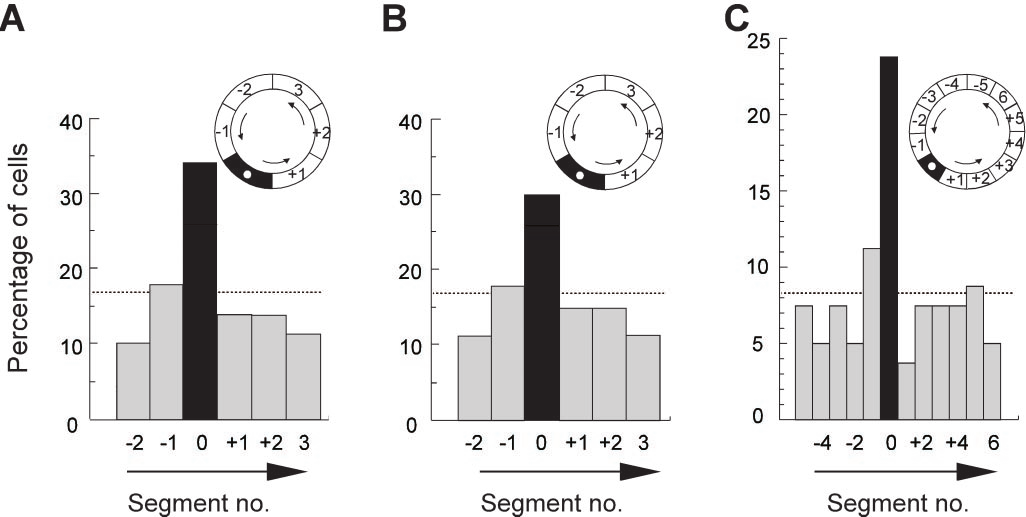
\includegraphics[width=0.7\textwidth]{intro/Hollup_accumulation}
	\caption[Distribution of firing fields from Hollup et al.]{Distribution of firing fields after training with a constant platform location.
	(A) Percentage of firing fields in each 60$^{\circ}$ segment of the corridor (80 cells; average of 3 probe tests). Field location was defined as the segment with the maximal averaged firing rate. Firing fields accumulated in the platform segment (segment 0, black). The chance level was at 16.7\%. Inset, Diagram of the corridor. Arrows indicate swim direction.
	(B) Percentage of firing fields in each 60$^{\circ}$ segment after directional sorting (same trials and same symbols as described in A). Only data sampled during swimming in the preferred direction are retained.
	(C) Percentage of firing fields in segments of 30$^{\circ}$ after directional sorting. The platform was in the middle of segment 0.
	Reproduced from \citet{Hollup2001a}.}
	\label{fig:intro:memory:hollup}
\end{figure}

Conceptually similar, but drier, are the Barnes or cheeseboard maze \citep{Barnes1979}\citep{Kesner1991}\citep{Dupret2010a}.
These mazes are consist of a large platform with holes throughout.
These holes can either be escapes for the mice/rats to avoid the exposure of the platform, or baited/rewarded.
Either way, the degree of learning can be quantified by latency to finding the correct location or time spent near previously rewarded locations during un-rewarded probe trials.
In a study by \citeauthor{Dupret2010a} which partially inspired my own work, the authors used a cheeseboard maze to examine hippocampal functional correlates of learning and memory (see \nameref{sec:df:methods:comp}).
They authors identified an increase in the fraction of hippocampal area CA1 place cells that encoded the reward location, the magnitude of which correlated with task performance (\autoref{fig:intro:memory:dupret}a,b).
In addition they found properties of sharp-wave ripples (SWRs) that also correlated with task performance -- the fraction of pyramidal cells that participated in sharp-wave ripple events during exploration (eSWRs) and the similarity of the pyramidal cell firing patterns during off-line SWRs (sSWRs) with on-line exploration of the reward locations (\autoref{fig:intro:memory:dupret}c,d).
In light of evidence pointing to a central role for SWRs in long-term memory consolidation \citep{Buzsaki2015}, it's tempting to interpret these findings as task performance being aided by an increased number of pyramidal cells encoding a memory of the reward locations during exploration and increased `remembering' of the rewarded locations during sleep.

\begin{figure}
	\centering
	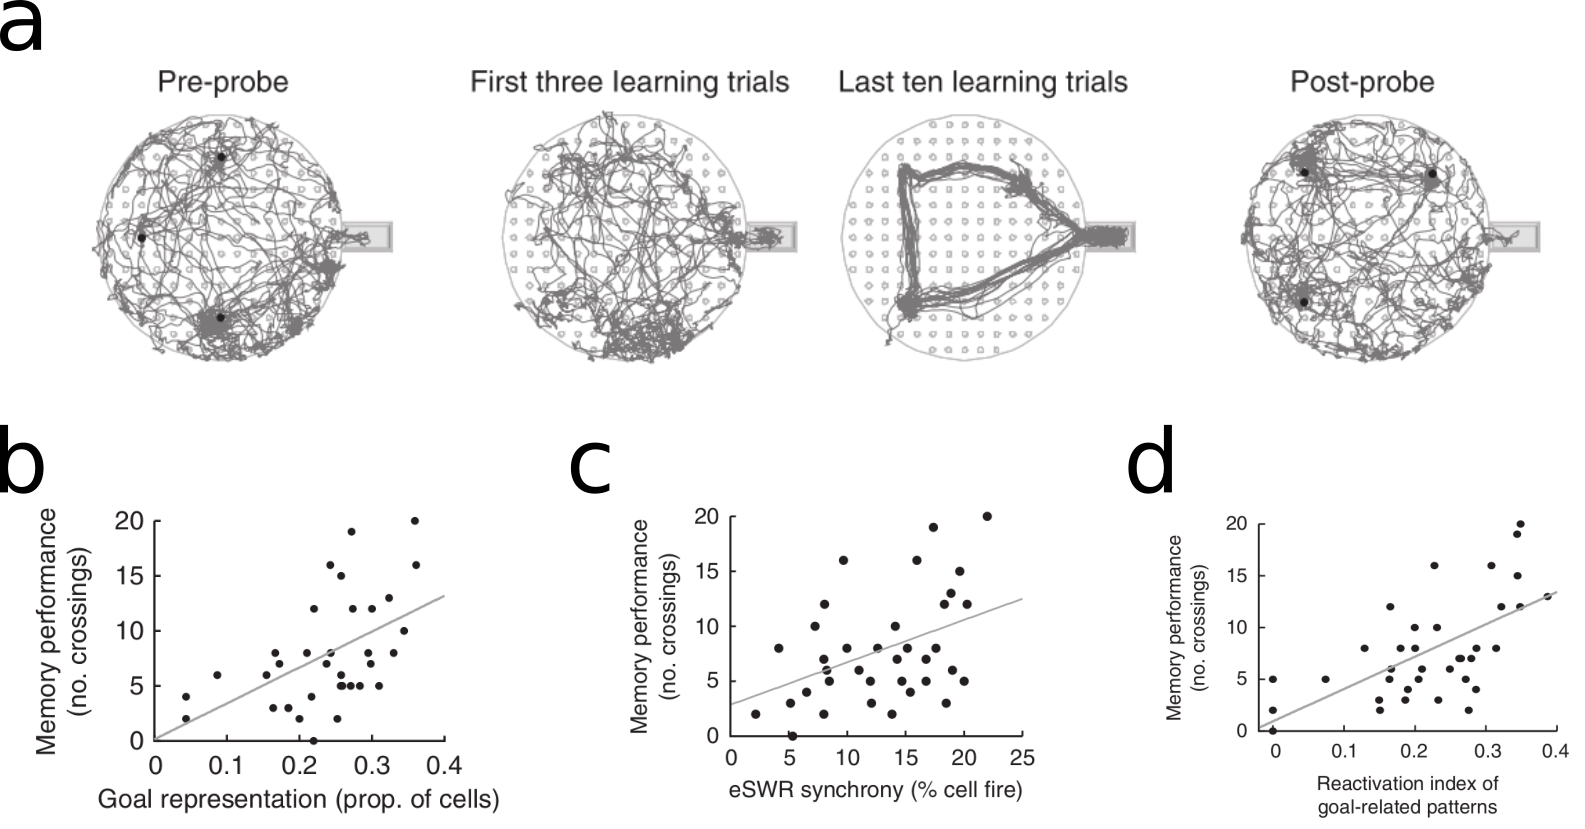
\includegraphics[width=0.7\textwidth]{intro/Dupret_cheeseboard_and_correlates}
	\caption[Cheeseboard task and behavioral correlates from Dupret et al.]{Cheeseboard task and behavioral correlates from Dupret et al.
	(a) Representative examples of an animal's path; for clarity, only the first 10 min of each probe session is depicted (black dots, learnt goal locations).
	(b) Scatter plot showing post-probe memory performance (number of crossings) as a function of the proportion of CA1 place cells at goal location during the end of learning (gray: regression line, r = 0.511, P=0.0014).
	(c) Scatter plot showing post-probe memory performance (number of crossings) as a function of `eSWR synchrony' (percentage of CA1 pyramidal cells that fire in eSWR) at the end of learning (gray: regression line, r = 0.418, P=0.011).
	(d) Scatter plot showing post-probe memory performance (number of crossings at a given goal location) as a function of the proportion of sSWRs in which assembly patterns represented the same goal location (gray: regression line, r = 0.620, P=0.00005)
	Figures rearranged and reproduced from \citet{Dupret2010a}.}
	\label{fig:intro:memory:dupret}
\end{figure}


\section{Memory in the brain}\label{sec:intro:memory:structure}
\todo{Expand more generally on brain regions involved in memory}

\subsection{The Hippocampus}\label{sec:intro:memory:hpc}
While `learning' in it's broadest sense is a fundamental feature of every neuron, in mammals, the \ac{HPC} is central to the formation, storage, and recall of explicit memories of experiences.
The \ac{HPC} has been central to our study of memory at least since Scoville and Milner first reported in the 1950's on Henry Molaison (patient H.M.) who had profound anterograde amnesia following the bilateral removal of large portions of the medial temporal lobes, which includes the \ac{HPC} and parahippocampal structures \citep{Scoville1957}.
\todo{Expand on patient HM}
Since then, numerous studies have shown that the \ac{HPC} is essential for normal formation and recall of long term episodic and semantic memory \citep[reviewd in][]{Eichenbaum2000, Burgess2002}.

The hippocampal is one of the best characterized neuronal circuits within the mammalian brain.
The principal neurons in the \ac{HPC} communicate through the classically-defined trisynaptic loop: perforant path fibers project from the entorhinal cortex (EC) to granule cells in the dentate gyrus, which in turn send mossy fiber projections to CA3 that finally travel along the Schaffer collateral pathway and synapse upon proximal apical and basal dendrites of CA1 pyramidal cells (CA1PCs).
CA1PCs then send processed information to cortical and subcortical areas, including return projections back to deep layers of EC.

Finally, both principal neurons and GABAergic interneurons are targeted by afferents from neuromodulatory nuclei, including cholinergic and GABAergic projections from the medial septum  \citep{Klausberger2008}, serotonergic and glutamatergic projections from the raphe nuclei \citep{Varga2009}, as well as dopaminergic and noradrenergic projections from the ventral tegmental area \citep{Gasbarri1997} and locus coeruleus \citep{Foote1983}.


Burwell RD (2000): The parahippocampal region: Corticocortical connectivity. Ann N Y Acad Sci 911:25–42.
\subsection{CA1}
\begin{figure}
	\centering
	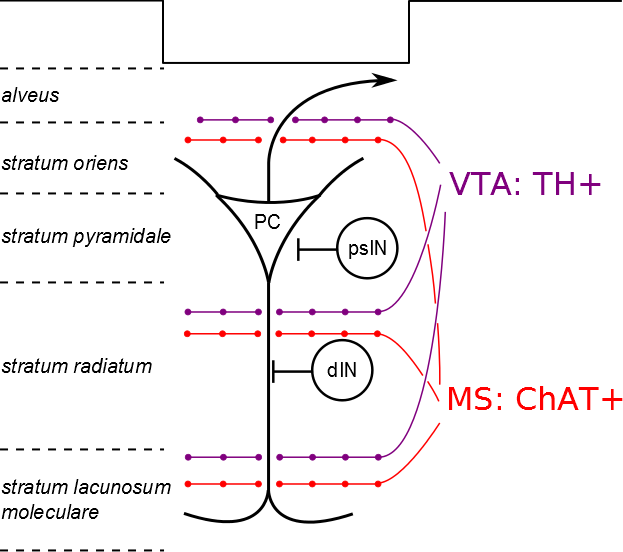
\includegraphics[width=0.5\textwidth]{intro/CA1-schematic_INs_VTA_MS}
	\caption{Schematic of major inputs to CA1 pyramidal cells}
	\label{fig:intro:memory:CA1_schematic}
\end{figure}


\subsection{Other}
In discussing the role of the \ac{HPC}, I've focused on spatial memory, but this is clearly not the sole role of the \ac{HPC}.
Social
Time
conversion to longterm memory
environment
pattern completion/separation

\section{Functional correlates of memory}\label{sec:intro:memory:physiology}

\subsection{Memory engrams}

\subsection{Spatial maps}
Perhaps the best-studied 
Throughout the \ac{HPC} (dentate gyrus, CA3, CA2, and CA1) there are principal cells that fire selectively at specific locations within an environment (\textsc{place cells}).
Our understanding of place cells is a uniquely well-characterized functional mapping of the real world multiple synapses from both sensory and motor cortices.

Within the entorhinal coretx, principal cells take on a variety of spatial firing properties, but one of the main categories are cells that fire at regularly spaced intervals throughout an environment (\textsc{grid cells}).
Place cells and grid cells together form the cellular foundation for the mammalian navigation system, and their discovery was recently awarded with the Nobel Prize in Medicine.
Pyramidal cells in hippocampal area CA1 are the principal excitatory neuron in that region and the primary output from the \ac{HPC}.
As an animal explores an environment these pyramidal cells show sparse spatially-modulated changes in firing rates (place cells) that are established rapidly and subsequently remain stable \citep{O'Keefe1971}\citep{Frank2004}.
These place cells form an allocentric map of the environment, which is essential for normal episodic memory function \citep{Smith2006c}\citep{Nakazawa2004}\citep{Buzsaki2013}.

\subsection{Place cells}\label{sec:intro:memory:place_cells}
\begin{figure}
	\centering
	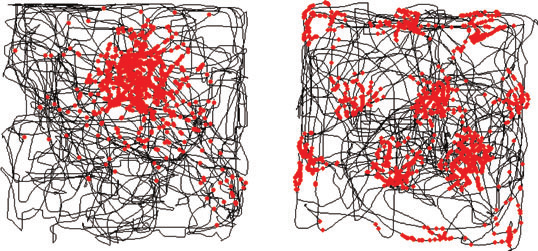
\includegraphics[width=0.7\textwidth]{intro/Moser_2008_place_grid}
	\caption[Place cell in the hippocampus and grid cell in the MEC]{Place cell in the hippocampus (a) and grid cell in the medial entorhinal cortex (MEC) (b).
	Spike locations (\emph{red}) are superimposed on the animal’s trajectory in the recording enclosure (\emph{black}).
	Whereas most place cells have a single firing location, the firing fields of a grid cell form a periodic triangular matrix tiling the entire environment available to the animal.
	Reproduced from \citet{Moser2008}.}
	\label{fig:intro:memory:place_grid}
\end{figure}

\subsubsection{Remapping}
\citep{Muller1987}
Place cells, like other forms of memory, are constantly trying to balance two competing constraints: on the one hand, their firing needs to be stable in order to be a helpful representation of the environment, but on the other hand, their firing needs to be plastic enough to constantly encode new environments, forget irrelevant information, and adapt to new features.
Place cells changing their firing properties to incorporate new features of the world is known as \textsc{remapping}.
A given place cell is defined by it's spatial tuning -- it's place field -- and it's firing rate gain with the place field.
These seem to be independent factors, as either can remap separately.
\textsc{Global remapping} is the collective remapping of place field locations across a population of place cells.
Alternatively, \textsc{rate remapping} is a change in place field gain (the ratio of firing rate in to out of the place field), while place fields locations remain fixed.
While place field location and firing rate gain remap separately....\textsc{partial remapping}.
\todo{Include Kentros}
\chapter{Schizophrenia}
\label{ch:intro:scz}

\section{Overview}
\Scz/ is a chronic, debilitating disease affecting approximately 1$\%$ of the population\citep{NIMHb}.
As the underlying aetiology is still poorly understood, \scz/ is defined by its symptoms, the most prominent of which is psychosis.
Symptoms are generally classified into three main categories: positive, negative, and cognitive \citep{Kay1982, NIMHa}.
Positive symptoms are behaviors not normally seen in healthy individuals and include hallucinations, delusions, suspiciousness, hostility, thought disorders, and movement disorders.
Negative symptoms reflect missing or disrupted normal thought processes, including: blunted affect, social withdrawal, avolition, anhedonia, and difficulty in abstract thinking.
Cognitive symptoms include attentional deficits, poor executive functioning, both working and long-term memory impairment, specifically in the domains of episodic semantic memory deficits.
While the positive symptoms, in particular hallucinations and delusions, might be the most prominent symptoms of \scz/, cognitive symptoms are present in up to 75$\%$ of \scz/ patients and the severity of cognitive symptoms is strongly linked to functional outcomes \citep{O'Carroll2000, Green1996, Keefe2007}.
This is particularly troubling since treatment options for the negative and cognitive symptoms of \scz/ are extremely limited.

Since the underlying causes of \scz/ are not known, treatment for patients with \scz/ is limited to treating symptoms as they present.
Treatment for \scz/ patients primarily includes a combination of antipsychotic medication and psychosocial therapy \citep{NIMHa}.
Patients’ responses to antipsychotics varies widely, some experiencing complete remission of psychoses and others showing no alleviation of symptoms.
Overall, following a first episode-psychosis, long-term antipsychotic treatment are effective in 30-40$\%$ of patients in preventing future psychoses \citep{Boyer2007, Insel2010}, leaving over half of all patients still experiencing psychotic events.
More importantly, antipsychotic medication only aim to treat the positive symptoms of \scz/, such as hallucinations and delusions.
Treatment options are extremely limited for the debilitating cognitive deficits - including deficits in attention, executive function, and both working and episodic memory, which have proven to be the greatest barrier to rehabilitation \citep{Lieberman2005, Harrison2001, O'Carroll2000, Hyman2003}.

In the following sections I will expand upon some of the symptoms, causes, and brain abnormalities observed in \scz/ patients, with a specific focus on aspects of the disease most relevant to my main research project: \autoref{ch:df}.
I will discuss details of the cognitive dysfunctions present in \scz/ patients [\ref{sec:intro:scz:memory}], with a particular focus on spatial and episodic memory impairments.
I will present what we do know about underlying genetic and environmental causes of \scz/ [\ref{sec:intro:scz:genes_and_environment}], including details of 22q11.2 deletion syndrome and a mouse model of this deletion, \df/.
Finally, I will lay out several proposed proximate causes of \scz/ symptoms including brain anatomical changes, alterations in neumodulatory signaling, and an imbalance in excitation and inhibition [\ref{sec:intro:scz:causes}].


\section{Memory deficits}\label{sec:intro:scz:memory}
Disruption in working and declarative memory are among the primary cognitive deficits observed in \scz/ patients.
The memory deficits present in \scz/ are specific in that patients seem to have relatively spared implicit or procedural memory, while many patients present with striking deficits in declarative memory, including both episodic memory (conscious recollection of events) and semantic memory (knowledge of people, place, objects, and facts) \citep{O'Carroll2000, Aleman1999, Gold2010}.
In addition to being specific, the observed memory deficits are also pervasive, in that they can not be accounted for by age, education, medication, disease duration or severity \citep{Ranganath2008} and are present in the majority of \scz/ patients \citep{}.
As mentioned more generally about cognitive symptoms of \scz/, the severity of memory impairments in particular is one of the strongest predictors of longterm functional outcome among \scz/ patients \citep{Green1996}, as failures in declarative memories provide the greatest barrier to steady employment.

The pattern of memory deficits observed in \scz/ patients is consistent with disruptions in both the executive control and memory strategies associated with the prefrontal cortex (PFC) as well as with the longterm memory storage function of the hippocampus (HPC).
Disorders that specifically arise from PFC lesions or dysfunction show a similar impairment in encoding and retrieval as seen in \scz/ patients \citep{Ranganath2008}.
Patients do not make use of the same semantic memory strategies as healthy individuals, though these impairments can at least in part be ameliorated by training in semantic memory strategies or through restructuring of task stimuli (e.g. blocked instead of unblocked word lists) \citep{Gold1992, Stone1998}.

\subsection{Spatial memory}
As described in more detail above (see \nameref{sec:intro:HPC:spatial}), memory for specifics locations is one particular type of episodic memory that has proven to be a tractable means for studying memory.
Spatial memory deficits are well documented in \scz/ patients \citep{Boyer2007, Hanlon2006, Aleman1999}, but the underlying circuit level dysfunctions have rarely been investigated \citep{Hayashi2015, Suh2013}.


\section{Genes and the Environment}\label{sec:intro:scz:genes_and_environment}
Significant recent advances in understanding \scz/ have come from identifying a large network of genetic abnormalities that predispose for \scz/.

\subsection{Schizophrenia as a neurodevelopmental disorder}\label{sec:intro:scz:neurodevelopment}

The typical age for a first psychotic episode is 18-25 years, though there is 

\subsection{22q11.2}
Evidence suggests that \scz/ has up to 80$\%$ heritability, and in particular, genetic studies have unequivocally implicated a region of human chromosome 22 (22q11.2) in disease risk \citep{Karayiorgou1995, Chow2006, Karayiorgou2010}.
Individuals with 22q11.2 microdeletions exhibit a spectrum of cognitive deficits as children, and $~$30$\%$ of them develop \scz/ in adolescence or early adulthood, accounting for up to 2$\%$ of all \scz/ cases \citep{Karayiorgou2010}.

\subsubsection{Df16}
Advances in understanding the genetic component of \scz/ predisposition have led to the development of etiologically-validated mouse models of \scz/ which will allow for the direct analysis of \emph{in vivo} neuronal network activity and identification of circuit dysfunctions present in the disease.
In order to dissect altered hippocampal circuitry in \scz/ I will be using the etiologically validated mouse model of the 22q11.2 microdeletion (\df/), generated by deleting the syntenic region in the mouse chromosome which contains most of the same 28 genes deleted in humans \citep{Stark2008}.
Behavioral tests on the \df/ mouse model have shown increased non-specific anxiety in open field and light-dark transition tasks, impaired sensorimotor gating by measuring startle response during prepulse inhibition (PPI), impaired spatial working memory in a delayed non-matching to place T-maze task, impaired working memory characterized by altered hippocampal-prefrontal synchrony, and decreased freezing in a contextual fear conditioning paradigm, which could reflect either impaired contextual memory or the inability to associate the unconditioned stimuli with the context in which it was presented \citep{Drew2011b, Stark2008, Sigurdsson2010}.
Additionally, a study of immediate early gene expression using c-Fos staining following exposure to a novel environment found significantly fewer CA3 pyramidal cells active and a trend in the same direction for CA1 pyramidal cells as well, which is suggestive of deficits in spatial memory \citep{Drew2011b}.
Taken together, the \df/ mouse model of the human \scz/-linked 22q11.2 microdeletion effectively recapitulates cognitive deficits seen in \scz/ patients, including increased anxiety, impaired executive control, and deficits in spatial and episodic memory.


\section{Mechanistic hypotheses}\label{sec:intro:scz:causes}
While the underlying cause of schizophrenia has remained elusive, collective evidence has pointed to several possible mechanistic pathways.
Narrowing down the disease etiology has been confounded by a high concordance with other psychiatric diseases.
Unlike Alzheimer’s disease or Parkinson’s disease where cell-death of specific cell types has been causally linked to disease progression, \scz/ and many other psychiatric disorders exhibit no drastic cell loss or increased gliosis, and affected brain regions can span both cortical and subcortical regions, suggesting network or circuit dysfunctions \citep{Uhlhaas2012, Lewis2002}.

\subsection{Anatomy}
Brain structural changes have been reliably identified in \scz/ patients following a first episode of psychosis, and more recently, in high-risk individuals during the prodrome, prior to a clinical diagnosis.
In particular, reductions in gray matter volume and a corresponding increase in lateral ventral volume have been consistently demonstrated \citep{Fusar-Poli2013, Shepherd2012}.
As we become aware of susceptibility genes, environmental triggers, and other prodromal markers of \scz/, the identification of an at-risk pool has allowed for the tracking of brain changes prior to the onset of psychosis.
Tracking of clinically high-risk individuals has identified \scz/-related structural changes in the hippocampal formation, the cerebellum, the superior and medial temporal lobe, the insular cortex and the prefrontal cortex \citep{Cannon2015, Millan2016}.
Additionally, among the clinically high-risk population, continued progression towards \scz/ can be predicted by monitoring gray-matter loss \citep{Tognin2014}, aiding in pre-symptomatic identification with the hope of early intervention treatments (see \nameref{sec:intro:scz:neurodevelopment}).

\subsubsection{Hippocampus}
Consistent behavioral, anatomical, and physiological studies of \scz/ patients have all pointed towards the HPC as an integral region in disease pathology \citep{Boyer2007, Bogerts1985, Jakob1986}.
Of these subcortical projections the medial septum projections are of particular interest, since the cholinergic projection has been linked to learning and memory \citep{Parent2004} and the GABAergic projection is known to target PV+ interneurons \citep{Freund1988} which are altered in \scz/ (see \nameref{sec:intro:scz:glutamate}) and it has also been linked to aberrant behavior in an NMDAR antagonist model of schizophrenia \citep{Ma2012}.
Despite these well-characterized features of hippocampal organization, it remains unknown how the function of these circuit motifs are altered in \scz/ during hippocampal-dependent behaviors.

\subsection{Dopamine}
The earliest mechanistic hypotheses for the disease progression of \scz/ involves disruption in normal dopamine signaling \citep{Matthysse1973}.
This hypothesis revolves around the positive symptoms of \scz/, specifically the hallucinations and delusions which can be both induced and prevented through modification of dopamine levels in the brain.
In particular, compounds that generally increase the level of dopamine (e.g. amphetamine, LSD) lead to hallucinations similar to those experienced by \scz/ patients \citep{Angrist1994, Lieberman1987}.
Conversely, for over 60 years the primary treatment for \scz/ has been antipsychotic medications \citep{Delay1952}, which were first shown to increase the metabolism of dopamine \citep{Carlsson1963} and are now known to function primarily as D2 dopamine receptor antagonists \citep{}.
The general effectiveness of classical antipsychotics (e.g. haloperidol) and the newer atypical antipsychotics (e.g. clozapine) in treating the positive symptoms of \scz/, suggested a central role for dopamine in the more general neuropatholysiology of \scz/, but this insight has failed to expand beyond the direct treatment of psychotic episodes.
Indeed, while D2 dopamine receptor antagonists work well for many patients in managing psychotic episodes, these treatments have done very little in improving functional outcomes, as the more debilitating negative and cognitive symptoms remain untreated \citep{Insel2010}.

The role of dopamine in \scz/ is now realized to be more nuanced than a simple consequence of a brain-wide hyperdopaminergic state.
While D2 dopamine receptor antagonist antipsychotic treatments do help manage psychotic episodes in many \scz/ patients, in some these treatments show no effect.
Additionally, post-mortem measurements of dopamine levels in \scz/ patients, as well as \emph{in vivo} measurements of dopamine activity, have not been entirely consistent across studies, and more importantly, across patients \citep{}.
This inconsistency is most likely reflective of variability in underly disease etiology, and points to a lack of a singular disease pathology, but rather a collection of underlying brain dysfunctions that funnel towards shared pathways and a commonly identified set of expressed symptoms.

Using radiolabeled L-dopa, presynaptic dopamine levels have been consistently shown to be elevated in the striatum of \scz/ patients \citep[for review, see][]{Howes2007}
At the same time, also in the striatum, D2/3 dopamine receptors (the primary receptor subtypes in this brain region) are modestly (10-20$\%$) elevated, independent of treatment with antipsychotic drugs \citep[for review, see][]{Howes2009}.
In contrast to the striatum, D1 dopamine receptors predominantly mediate dopamine activity, and while the effect is not as consistent, receptor levels show an association with severity of cognitive and negative symptoms in \scz/ \citep{Goldman-Rakic2004}.


D2r presynaptic striatum

hypodopamine frontal?

dopamine spcific to psychoses

many underlying causes that converge on dopamine (complex genetic interactions and environmental hits)

subcortical hyperdopaminergia, prefrontal hypodopaminergia

\subsection{Glutamate/GABA}\label{sec:intro:scz:glutamate}
It has been proposed that an imbalance in levels of excitatory and inhibitory activity during development underlies \scz/ \citep{Insel2010, Coyle2006, Yizhar2011}.
Support for this theory includes the observation that NMDA receptor (NMDAR) antagonists, such as phencyclidine and ketamine, induce psychoses in healthy subjects \citep{Morris2005}, worsen symptoms in \scz/ patients, and cause schizophrenia-like symptoms in mice \citep{Inta2010}, while agonists for the NMDAR glycine binding site show potential to alleviate symptoms \citep{Tsai1998}.
Additionally, post-mortem studies have found decreased levels of pre-synaptic GABAergic machinery, including GAT, GAD67, and parvalbumin (PV), in both the prefrontal cortex (PFC) and HPC \citep{Coyle2006, Zhang2002, Konradi2011}.
In particular, \scz/ patient have shown decreased levels of parvalbumin leading to hypofunction of PV+ interneurons in the prefrontal cortex as well as decreased numbers of PV+ interneurons in the HPC \citep{Zhang2002, Lewis2005} and parvalbumin interneurons are required for normal spatial working memory functions \citep{Korotkova2010, Murray2011}.
However, there is currently limited data available on how activity of hippocampal GABAergic interneurons is altered in \scz/.

\chapter{Techniques}
\label{ch:intro:techniques}
\acresetall
\chapter{Techniques}
\label{ch:intro:techniques}

\section{\emph{In vivo} two-photon Ca\super{2+} imaging}
All of my experiments revolved around two-photon Ca\super{2+} imaging in hippocampal area CA1 of head-fixed mice using genetically-encoded calcium indicators (GECIs), in particular GCaMP6f.
In vivo Ca{2+} imaging allowed me to record the activity of hundreds of pyramidal cells or multiple axonal projection fibers simultaneously and, importantly, follow the same cells or fibers for multiple days.
During my thesis work, the most significant upgrade to our imaging capabilities was the addition of resonant scanning capabilities, which increased our imaging rate by roughly a factor of 10.
This allowed for up to a 10 times increase in both temporal and spatial resolution, which greatly improved the quality of our imaging data.
The upgrade also required a corresponding upgrade to our analysis pipeline and server design to handle the significantly increased quantity of data acquired (see below).

\section{Head-fixed behavior}\label{sec:intro:techniques:behavior}
In order to allow for two-photon Ca\super{2+} imaging in awake mice, we need to design all behavioral tasks to work while mice are head-fixed under a two-photon microscope.
While the core apparatus was in place when I began experiments, extensive upgrades were necessary to optimally run my head-fixed learning tasks.
I, along with colleagues in the lab, redesigned the wheels, axles, and platform to minimize friction and facilitate running while head-fixed.
We designed a RFID-tag and quadrature encoded-based system to accurately track position over many laps to within $<$0.5~cm.
We designed new treadmill belts that consist of multiple fabrics sewed together with various cues scattered throughout, which together convey all the spatial information used by mice to anchor place cell maps.
I added features to our in-house behavioral control software to allow for the presentation
These hardware changes allowed for the design of new head-fixed behaviors, described below.

\subsection{Random foraging}
The first task we designed was a simple random foraging task where mice run to get water, but don't need to learn about any particular location on the belt in order to get water rewards.
All head-fixed paradigms begin with 1-2 weeks of training where mice learn to lick for water from a lick port while needing to run progressively farther in order to receive another reward (see \autoref{sec:df:methods:training}).
Mice were either operantly rewarded (they must lick to receive water) at random intervals along the belt or non-operantly at a fixed location.
This allowed me to look at baseline stability of spatial maps with two-photon Ca\super{2+} imaging over days or weeks (see \autoref{sec:applications:chronic}).

\subsection{Goal-oriented learning}\label{sec:intro:techniques:GOL}
In order to study spatial learning and memory while simultaneously imaging functional activity of hippocampal area CA1 place cells, I developed a head-fixed \ac{GOL} task.
Freely-moving assays of spatial memory in rodents traditionally include the Morris water maze, Barnes maze, or cheese board maze (see \autoref{sec:intro:memory:spatial-reward}).
While head-fixed under a two-photon microscope, mice are constrained to run in effectively a one-dimensional environment (similar to freely moving linear track paradigms) and there are limited options to experimentally assay choices made by the mice.
They key features that we were trying to design in the task were:
\begin{enumerate}
	\item Mice are able to learn a specific rewarded location on the treadmill that is otherwise un-cued.\label{item:into:techniques:GOL:location}
	\item Mice learn the task over several trials to allow for determining a `learning curve'.\label{item:into:techniques:GOL:learning}
	\item A behavioral readout that is sensitive to subtle variations in ability to learn.\label{item:into:techniques:GOL:readout}
	\item Be able to flexibly manipulate the reward and environment parameters to probe mice' ability to learn the task.\label{item:into:techniques:GOL:manip}
\end{enumerate}

Our \ac{GOL} task requires mice to run laps along our multi-fabric, feature-rich circular treadmill belt.
The mice are water-restricted, so we use water delivered through a lick port as a reward.
Each lap there is one spatial region (\textsc{reward zone}, usually a 20-cm window) on the belt where the mice can operantly receive water rewards: if they lick they get water, if they do not lick, they don't.
The reward will `dry up' after after a fixed amount of time has passed since the mouse entered the reward zone that lap (usually 3 seconds).
Not all mice will run for water rewards at all, and not all mice will perform this task, but many are able to (\ref{item:into:techniques:GOL:location}).
We generally give the mice 9 sessions to learn the reward location.
Some mice will find the reward immediately, but even those that do, they continue to improve and stabilize their performance over the 9 sessions (\ref{item:into:techniques:GOL:learning}).
By measuring the capacitance of the lick port, we can detect changes when the mouse licks, providing us an accurate measure of the time (and the mouse's location on the belt) when each lick occurs.
The operant nature of the reward schedule requires the mice to lick everywhere along the belt to sample each location and find the correct position that will be rewarded.
As the mice learn the reward zone, they suppress licking away from the reward and will then only lick at the reward zone.
We have used multiple measures to quantify this behavior, but generally look at the fraction of licks in the reward zone as a measure of learning (\ref{item:into:techniques:GOL:readout}).
This particular measure can be misleading if the mice lick everywhere along the belt, but then lick robustly once they receive the first drop of water, but in practice we do not see this behavior.
In addition we often look at measures such as \textsc{anticipatory licking}, which quantify the fraction of licks directly preceding the reward, but crucially exclude licks in response to water delivery, though this measure has proven to be less-sensitive to learning.
Finally, the setup allows the experimenter to move the reward to any arbitrary location along the belt, swap out belts to modify the environment, and manipulate non-spatial odor/tone/light cues to change the surrounding context (\ref{item:into:techniques:GOL:manip}).

\section{Data analysis pipeline}\label{sec:intro:techniques:pipeline}
A typical 10 minute imaging session generates a $\approx$15~GB raw movie that needs to be processed down to a single spatial tuning vector for each of approximately 500 cell somas in the field of view.
Processing each movie requires identifying regions of interest (ROIs), extracting fluorescent signals from each ROI, cleaning up each trace by calculating changes in fluorescence, identifying significant Ca\super{2+} events, aligning Ca\super{2+} event times to the mouses' position in the behavioral environment, and finally calculating place fields for each cell.
Place fields from a single session can tell us how the mice represent the environment in a given session, but to address some of the more interesting questions I wanted to ask how these representations changed over time.
For this, I needed to register ROIs from day-to-day and compare the tuning of the population as a whole over time, but also track changes in the tuning of individual pyramidal cells from session-to-session.
All of these steps need to be performed fast, reliably, and as automatically as possible.
Over the course of my PhD thesis work, I, along with other members of Attila's Lab (especially Patrick Kaifosh and Nathan Danielson), developed a set of programs and tools to complete all of these steps mentioned above.
I will focus here on the pieces that I personally originated or was the primary contributor to, but ``no man is an island''; Attila's lab is collaborative by design and all the code we use is shared, so multiple people have contributed to most aspects of the analysis pipeline.

\begin{figure}
	\centering
	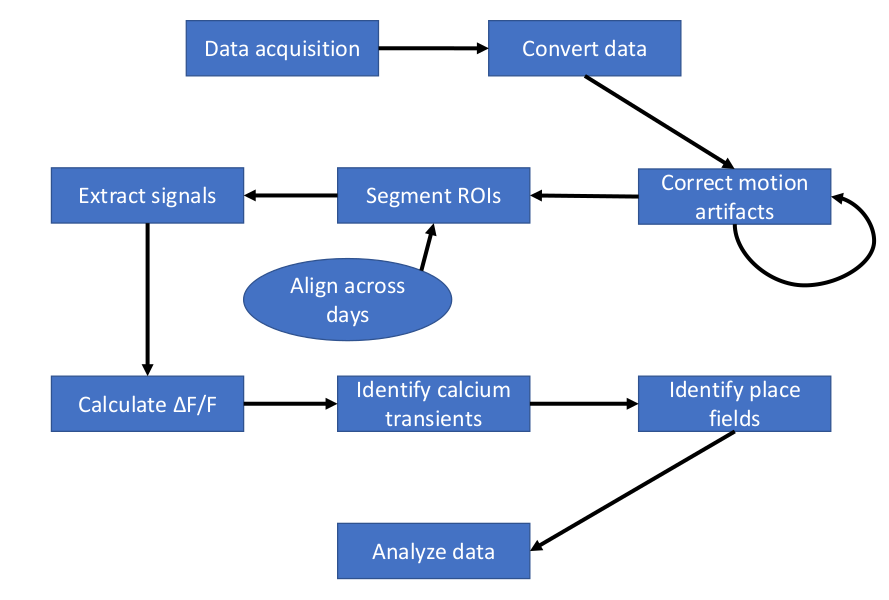
\includegraphics[width=0.9\textwidth]{intro/data_pipeline}
	\caption[Data analysis pipeline]{Data analysis pipeline. Schematic represents the various steps of processing performed on all data.}
	\label{fig:intro:techniques:pipeline}
\end{figure}


\subsection{Initial processing}\label{sec:intro:techniques:inital}
Imaging data acquired through our microscope software (PraireView) is stored as an individual TIFF image file for every frame of every plane and channel.
This can lead to over 30,000 files per 10 minute recording session, which very quickly becomes difficult to manage.
So, the first step after running an experiment is to move all the data to a special \textsc{scratch} folder on our lab server, where I have a script constantly running to convert all of the data into one large HDF5 file (\url{https://www.hdfgroup.org/HDF5/}).
This format allows us to store all of the data in a 5-dimensional (Time $\times$ Plane $\times$ Row $\times$ Column $\times$ Channel) indexable structure for easy iteration and viewing of the data.
The script checks every individual TIFF file, writes it to the HDF5 file, verifys the integrity of the new HDF5 file, and then moves the new file to a permanent place on the server while deleting the original TIFF files.

At this point the data is now properly formatted for estimation and correction of motion-induced imaging artifacts using our SIMA software package (\autoref{ch:sima}).

% \subsection{Signal extraction}

\subsection{Signal processing}
After signals are extracted for each ROI the next step is to quantify the change in fluorescence over time, as absolute fluorescent values are not interpretable in isolation.
Calculating the change in fluorescent over time is simple in theory: $$\Delta F/F(t) = \frac{F(t) - F_{\circ}}{F_{\circ}},$$ though in practice there are many complications that any algorithm needs to be robust to.
The primary concern is a non-stationary baseline fluorescence, as drift in the baseline intensity can be mistaken for physiological activity, when in fact it is usually due to an experimental artifact.
The most common problem is for the baseline to decay over the course of long recordings, caused by water evaporation/leaking from under the objective, bleaching of the Ca\super{2+} indicator, movement of the tissue out of focus, or some combination of these factors.
While not particularly common, these things do occur and thus need to be accounted for.

Our particular baseline calculation method is based off of \citet{Jia2011}.
In brief, we first smooth the signal with a boxcar smoothing window of width $\tau_1$ and then for every time-point choose the baseline to be the minimum value of this smoothed signal within a $\tau_2$ window.
This effectively implies that there should be a $\tau_1$ size window every $\tau_2$ seconds that is absent of any Ca\super{2+} transients or other large fluctuations.
For hippocampal area CA1 pyramidal cells imaged with GCaMP6f in a well-trained mouse running on a 2-meter long treadmill, we found that $\tau_1$ = 3 seconds and $\tau_2$ = 60 seconds worked well.
As an additional step to aid the robustness of the precise window sizes, we also implemented an iterative procedure where after calculating $\Delta F/F$ we identified significant Ca\super{2+} events (see \autoref{sec:df:methods:transients}) and then re-calculated the $\Delta F/F$ while removing the identified Ca\super{2+} transients from the baseline.
This prevents errors in the baseline calculation for any cells that do not have a 3 second period of quiescence every minute, and was generally repeated 3 times to ensure an accurate baseline calculation.

\subsection{Place cell identification}
Pyramidal cells in the mammalian hippocampus fire at specific locations within a familiar environment.
We developed an algorithm to reliably identify cells that had a significantly higher mutual information between the mouse's position and the Ca\super{2+} activity of the cell than expected by chance.
The overall goal of our analytical approach is to identify as un-­biased a population of spatially-­tuned cells as possible.
In particular, we aim to avoid biases in place  field width, number of place fields per cell, location of place fields on the belt, or overall cell activity/firing rate level.
In addition, unlike with electrophysiological data, Ca\super{2+} events have a finite duration that we needed to account for on a per-­cell basis.  

In brief, we calculate the occupancy normalized transient rate histogram for each cell with bin sizes ranging from 2~cm to 100~cm.
In addition, for each bin size we also rotate the binning through all the possible shifts, such that, for example, if a cell fired transients over any continuous 20~cm segment of the belt, there would be a 20~cm bin that contained all of the transients.

We then calculate the spatial information for each of these bin sizes and bin shifts and take the maximum value as the true spatial information of that cell.
We then shuffle all of the transients within each cell, re-­calculate the occupancy normalized transient rate histogram for each bin size and shift as described above, again take the maximum spatial information for this particular shuffle, and then create a distribution of spatial information values across shuffles.
This distribution empirically defines our spatial information confidence threshold for the particular pattern of transient durations and timings for the particular cell.

Additional details of this method can be found in \autoref{sec:df:methods:pc_identification}.
 
\subsection{Lab Analysis Bundle (LAB)}
Over the years, as the lab and our code base grew, the collection of scripts, classes, and functions used for our analysis became hard to mention and difficult for new members to learn.
In order to stabilize the code for future members, I spearheaded an effort to clean-up, refactor, and document all of the code we used in the lab.
This became the Lab Analysis Bundle (LAB), which is a complete Python package hosted privately on GitLab (\url{https://gitlab.com}).
The package is easily installable using standard Python packaging tools, with well-defined dependencies.
As part of refactoring the code, I added automatic documentation to the core functions and standardized the API.
The lab code repository is now in a much more manageable structure that has successfully been passed on to future lab members.

The LAB contains all of the tools needed to analyze behavior and imaging data acquired in Attila's lab.
The core components are:
\begin{itemize}
	\item{Standardized representation of all experimental \textbf{metadata}, including mouse information, experiment start time, and exact behavioral parameters.}
	\item{Scripts for \textbf{processing} of imaging data from raw movies to extracted traces for each ROI.}
	\item{Access to all of the \textbf{behavioral data} acquired during the experiment, such as licking and position information.}
	\item{Object-oriented \textbf{structure} to work with collections of mice and experiments.}
	\item{\textbf{Analysis methods} to calculate behavioral (e.g. fraction of licks near rewards) and functional (e.g. place field correlation) metrics.}
	\item{Generalized \textbf{plotting} functions that work the output of any analysis function.}
	\item{\textbf{Automatic analysis scripts} to quickly perform standard analyses as soon as imaging data is processed.}
\end{itemize}

Below is an example analysis that will plot a histogram of place field widths for all recorded sessions from one mouse.

\begin{lstlisting}[language=Python]
import matplotlib.pyplot as plt
import lab

# Parse experiments metadata
expts = lab.ExperimentSet('behavior_jeff.xml')
# Pull out one particular mouse
mouse = expts.grabMouse('jz119')
# Find all sessions that were imaged
expt_grp = lab.classes.pcExperimentGroup(mouse.imagingExperiments())

# Calculate the width of all place fields
pf_width = lab.analysis.place_cell_analysis.place_field_width(expt_grp)

# Plot a histogram of all the place field widths
ax = plt.axes()
lab.plotting.plot_dataframe(
	ax, [pf_width], plot_method='hist', labels=['jz119'],
	activity_label='Place field width (cm)')

\end{lstlisting}

\begin{figure}[!h]
	\centering
	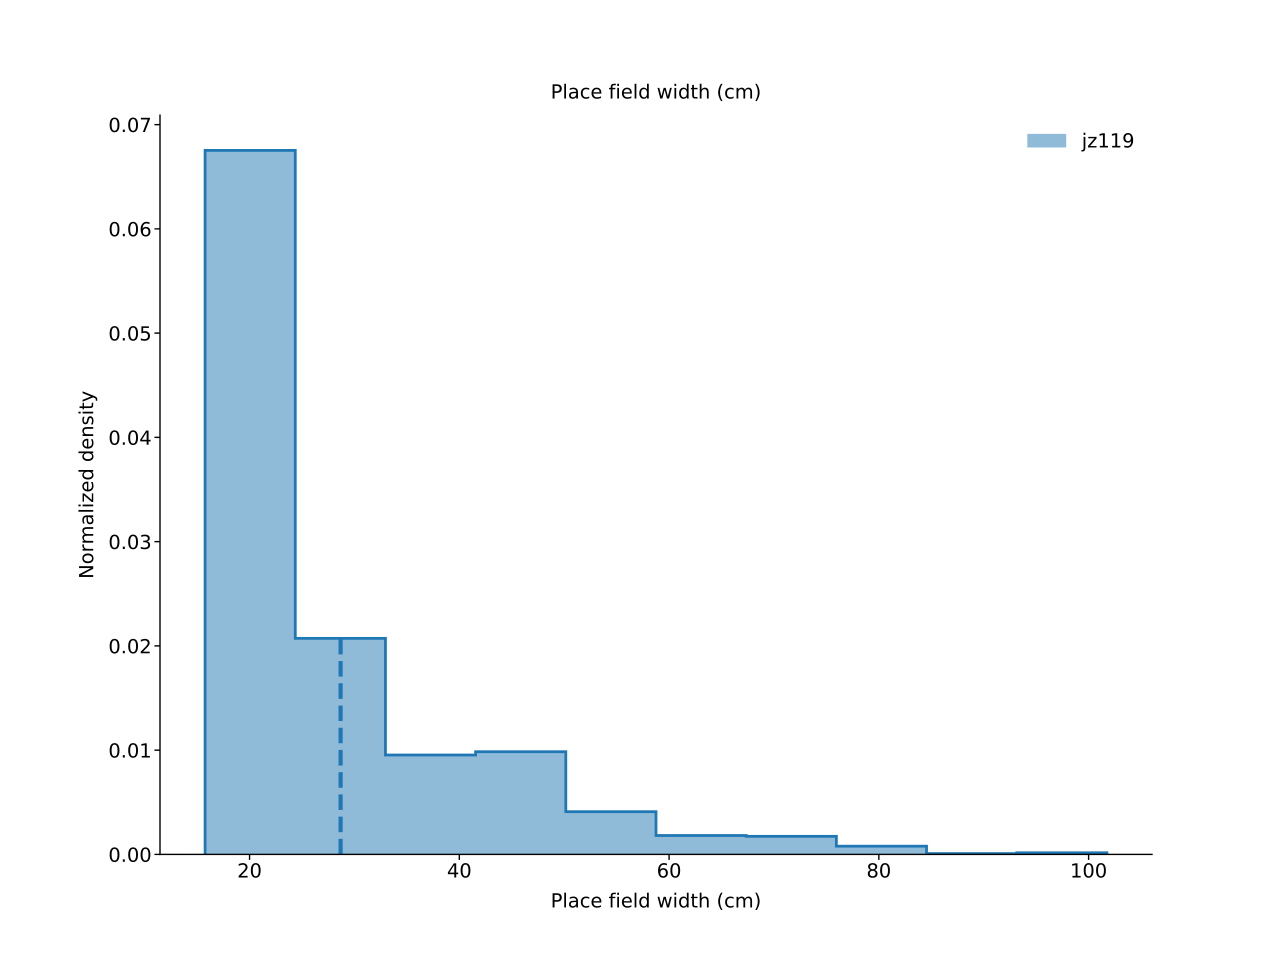
\includegraphics[width=0.7\textwidth]{intro/LAB_pf_width_example}
	\caption[Example histogram]{Example of using LAB to collect experiments, calculate a place cell metric, and plot the data.}
	\label{fig:intro:techniques:pf_width}
\end{figure}


\subsection{Place cell stability}\label{sec:intro:techniques:place-cells}




\part{Approaches}
\newcommand{\df}{}
\def\df/{\emph{Df(16)A\super{+/-}}} % Enforces that the command is ended with / and doesn't consume the trailing space
\newcommand{\Aprime}{}
\def\Aprime/{Context~A\super{$\prime$}}
\newcommand{\A}{}
\def\A/{Context~A}

\chapter[Impaired hippocampal place cell dynamics in a mouse model of the 22q11.2 deletion]{Impaired hippocampal place cell dynamics in a mouse model of the 22q11.2 deletion\footnote{This is joint work with the coauthors.}}
\label{ch:df}

Hippocampal place cells represent the cellular substrate of episodic memory. While place cell ensemble activity reorganizes to support learning, place cells must also maintain stable representations to facilitate memory recall. Despite extensive research, the learning-related role of place cell dynamics in health and disease remains elusive. We employed chronic two-photon Ca\super{2+} imaging in hippocampal area CA1 of wild-type and \df/ mice, an animal model of 22q11.2 deletion syndrome, one of the most common genetic risk factors for cognitive dysfunction and schizophrenia. We found that goal-oriented learning in wild-type mice was supported by stable spatial maps and the robust remapping of place fields toward the goal location. \df/ mice showed a significant learning deficit, and this finding was accompanied by both a reduction of spatial map stability and the absence of goal-directed place cell reorganization. These results expand on our understanding of hippocampal ensemble dynamics supporting cognitive flexibility during learning and provide the first direct demonstration of their disruption in a model of 22q11.2-associated cognitive dysfunction.

\section{Introduction}

Episodic memory, the encoding of personal experience organized in space and time, represents a fundamental aspect of cognition, crucial for learning about the world and normal functioning in everyday life. Episodic memory dysfunction, stemming from the inability to learn and recall contextual, spatial, and temporal details of specific events \citep{Dickerson2010, Eichenbaum2000}, is a highly debilitating symptom of various neurological, cognitive and psychiatric disorders, including schizophrenia (SCZ) \citep{Dere2010, Leavitt2009}. In the case of SCZ, episodic memory impairments are consistently reported \citep{Aleman1999, Schaefer2013} and largely untreatable \citep{Green1996, Ibrahim2011, Keefe2007}. More generally, cognitive deficits in SCZ appear to be the strongest predictor of patients’ functional outcomes irrespective of the underlying disease etiology \citep{Green1996, Ranganath2008}. Understanding the neural circuit dynamics that supports episodic memory and the manner in which it fails will provide vital clues to the understanding and treatment of cognitive deficits in psychiatric disorders.

To this end, we studied a well characterized animal model of cognitive dysfunction and SCZ, the \df/ mouse model of the 22q11.2 deletion syndrome (22q11.2DS). 22q11.2 deletions are responsible for variable childhood cognitive deficits and behavioral phenotypes as well as adult psychiatric illness, most notably SCZ \citep{Biswas2016, Schneider2014}. Deletion carriers have a 30-fold increased risk to develop SCZ, accounting for 1–2$\%$ of cases of sporadic forms of the disease \citep{Karayiorgou2010, Xu2008} and there are no major clinical differences in the core SCZ phenotype between individuals with SCZ who are 22q11.2 deletion carriers and those who are not \citep{Bassett2003}\citep{Bassett1998}. Importantly, \df/ mice, recapitulate many cognitive and behavioral deficits seen in 22q11.2 deletion carriers and SCZ patients in general, as well as disease-related anatomical and functional alterations in the hippocampus and frontal cortex \citep{Glausier2013}\citep{Scariati2016}\citep{Schmitt2015}\citep{Schmitt2016}\citep{Spencer2004}\citep{Uhlhaas2010}\citep{Weinberger2016}. These alterations include deficits in synapse formation, plasticity, and long-range functional connectivity \citep{Drew2011b}\citep{Mukai2008}\citep{Stark2008}\citep{Fenelon2013}\citep{Mukai2015}\citep{Sigurdsson2010}\citep{Tamura2016}, pointing to the conservation of disease pathways across species and enabling the formulation of specific hypotheses for underlying psychopathology.

Cognitive dysfunction in SCZ patients manifests as deficits associated with several spatial memory domains, such as deficits in spatial navigation reference memory, spatial working memory, and episodic memory \citep{Hanlon2006}\citep{Piskulic2007}\citep{Ranganath2008}\citep{Schaefer2013}\citep{Wilkins2013}. Furthermore, SCZ is linked to impaired performance in basic spatial tasks, such as the mental rotations of letters and objects \citep{DeVignemont2006} and also to more complex tasks \citep{Landgraf2011}\citep{Weniger2008}, such as visuo-spatial working memory \citep[see review][]{Piskulic2007}. In particular, patients with SCZ have an impaired ability to process contextual information \citep{Barch2003}\citep{Cohen1999}\citep{Maren2013}, frequently exhibit perseverative behaviors in tasks requiring cognitive flexibility \citep{Crider1997}\citep{Leeson2009}\citep{Morice1990}, and a failure to switch between cognitive strategies in spatial, relational and associative memory tasks \citep{Armstrong2012}\citep{Hanlon2006}\citep{Sheffield2012}\citep{Wilkins2013}.

The well documented role of the hippocampus in spatial and episodic memory \citep{Burgess2002}\citep{Buzsaki2013}\citep{Dickerson2010}\citep{Eichenbaum2000}\citep{Eichenbaum2014}, combined with morphological and functional alterations of the hippocampus in SCZ patients \citep{Narr2004}\citep{Vita2006}\citep{Witthaus2010}\citep{Zhou2008}\citep{Heckers2010}\citep{Meyer-Lindenberg2005}\citep{Tamminga2010}\citep{Collin2011}\citep{Debbane2006}\citep{Flahault2012} and disruptions in functional connectivity \citep{Harrison2001}\citep{Hutcheson2015}, collectively point to a central role for the hippocampus in the pathophysiology of cognitive memory deficits in SCZ \citep{Achim2005}\citep{Bast2011}. In particular, physiological and morphological alterations are reported specifically in hippocampal CA1 output node in SCZ patients \citep{Narr2004}\citep{Zierhut2013}, suggesting a potentially primary role for area CA1 in hippocampal pathophysiology in SCZ. Nevertheless, learning-related neural population dynamics under pathological conditions remain largely unexplored.

Neural circuits in the mammalian hippocampus support episodic memory by providing cognitive representations of spatial and contextual aspects of an experience \citep{Burgess2002}\citep{Buzsaki2013}\citep{Eichenbaum2000}\citep{O'Keefe1971}. At the neuronal level, principal cells in the hippocampus are selectively active in specific locations within an environment (place cells) \citep{O'Keefe1971}, forming the cellular basis of the fast high-capacity declarative memory system \citep{Buzsaki2013}. At the ensemble level, place cells collectively form cognitive maps of space \citep{Hartley2014}\citep{Leutgeb2005c}\citep{O'Keefe1971}\citep{OKeefe1978}\citep{Moser2015}, which are proposed to be expressions of individual memories \citep{Moser2015}\citep{Buzsaki2013}, and the long-term stability of hippocampal spatial representation is a widely posited prerequisite for reliable spatial learning \citep{Kentros2004}\citep{Lever2002b}\citep{Mankin2012}\citep{Thompson1990}\citep{Ziv2013}. Consistent with this view, place cells modify their preferred firing fields to incorporate both contextual \citep{Colgin2008}\citep{Karlsson2008}\citep{Leutgeb2005a}\citep{Leutgeb2004}\citep{Muller1987b}\citep{Wilson1994} and non-spatial information, including salient sensory information, as well as internal state of the animal \citep{Frank2000}\citep{Kobayashi1997}\citep{Moita2004}\citep{Pastalkova2008}\citep{Wood1999}, while at the same time, place maps are also modulated by proximal cues in an environment, which can serve as local landmarks to support allocentric navigation \citep{Deshmukh2013}\citep{Knierim2011}\citep{Knierim2003}. Importantly, it has been repeatedly demonstrated that place maps incorporate goal-related information during learning \citep{Breese1989}\citep{Fyhn2002}\citep{Dupret2010a}\citep{Gothard1996}\citep{Hok2007}\citep{Hollup2001b}\citep{Kobayashi1997}, and that place coding is altered during behaviors requiring increased attention \citep{Kentros2004}\citep{Markus1995}\citep{Muzzio2009a}. In particular, goal-directed reorganization of place cells was found to predict  memory  performance \citep{Dupret2010a}. Therefore, monitoring hippocampal ensemble dynamics provides a tractable entry point for understanding – at the cellular and neural population levels – how genetic mutations associated with cognitive dysfunction and psychiatric disorder lead to circuit abnormalities and the emergence of learning deficits.  While studies have examined the role of place cells in supporting spatial and episodic memory, the roles of spatial map stability and plastic reorganization of place cell populations during learning remain poorly understood, especially as they relate to disease-associated cognitive dysfunction. 

Two-photon Ca\super{2+} imaging during head-fixed behaviors \citep{Danielson2016b}\citep{Dombeck2010} allows for the chronic recording of physiological activity from individual CA1 place cells, as well as their ensemble activity as a whole. Chronic imaging provides a unique opportunity to follow changes in individual place cells over days and understand how a SCZ-related mutation affects local activity in the final output node ream of the hippocampus. In light of the well documented deficits in memory functions and cognitive flexibility in SCZ, we aimed to develop a spatially-guided reward learning task for head-fixed mice, during which task demands could be readily switched from initial reward learning in a novel context, to maintenance of a reward location memory following context manipulation, and finally to learning a new reward location in a now familiar context. By tracking the activity of hippocampal area CA1 place cell populations with chronic two-photon Ca\super{2+} imaging in \df/ mice and wild-type (WT) littermates through each phase of this learning task, we identified specific aspects of place cell map stability that evolved with learning, as well as alterations in the stability and plasticity of these cognitive maps in the mutant mice. In addition, we analyzed place cell maps during random foraging in a task-free context and found that the spatial map stability differences were specific to the more cognitively challenging learning conditions. Our findings highlight the reduced stability and impaired goal-directed reorganization of hippocampal place cells as fundamental components of 22q11.2 deletion-linked cognitive dysfunction.  

\section{Results}

\subsection{Head-fixed goal-oriented learning paradigm}
We injected mice with AAV1/2(\emph{Synapsin-GCaMP6f}) in dorsal hippocampal area CA1 to express the genetically-encoded Ca\super{2+} indicator GCaMP6f \citep{Chen2013} in neurons located in the CA1 pyramidal layer (see \nameref{sec:methods:mice}).  Mice were implanted with a head-post and imaging window to provide long-term optical access to the CA1 pyramidal layer \citep{Danielson2016b}\citep{Kaifosh2013}\citep{Lovett-Barron2014}.  In order to facilitate chronic two-photon functional imaging from hippocampal CA1 place cells \citep{Danielson2016b}\citep{Dombeck2010} during learning of a spatial navigation task, we used a head-fixed variation of goal-oriented learning \citep{Danielson2016b} (GOL, Fig. 1a) tasks that have been previously used in freely-moving rodents \citep{Dupret2010a} (see \nameref{sec:methods:comp}).  For this, we first trained water-deprived mice to run on a linear treadmill \citep{Danielson2016a}\citep{Danielson2016b}\citep{Royer2012} and then on the first day of the experiment introduced the mice to a novel environmental context, consisting of a feature-rich fabric belt and specific background non-spatial odor, tones, and blinking light patterns (Fig. 1a). Operant water rewards were available at a single unmarked location on the belt; if the mouse licked in the correct location they received a water reward, but no water was administered if they did not lick in the reward location or if they licked outside the reward location (Condition~I, 3 days, 3 sessions per day).  We recorded the time of each lick as well as the position of the mouse on the treadmill in order to both determine when to deliver water rewards and to provide a readout of learning. As the mice learned the reward location they switched from exploratory licking along the entire belt, to focused licking only at the reward location, suppressing licking at other locations (Fig. 1b). In order to test the ability of mice to adjust to changes in the task conditions, we challenged mice by exposing them to an altered context (same sequence of belt materials, shuffled local cues, different non-spatial odor, tone, and light, see \nameref{sec:methods:contexts}), while maintaining the same reward location relative to the belt fabric sequence (Condition~II, 3 days, 3 sessions per day). During the last part of the task, we changed the location of the hidden reward while maintaining the familiar context from Condition~II (Condition~III, 3 days, 3 sessions per day). As a point of clarity, we use the term “context” to refer to the entire environment and set of features present during the experiment, including the fabric belts, local cues, non-spatial odor, tone, and light, the head-fix apparatus and the microscope itself, but importantly not the un-cued reward location. Also, “position” is always in reference to the sequence of three distinct belt fabrics, which were always in the same order throughout all Conditions of the experiment.

\subsection{\df/ mice are impaired in GOL task following changes in both context and reward location}

Our overall behavioral analysis on the GOL task revealed general differences among genotypes (Two-way RM ANOVA all days and conditions, main effect of genotype: p=0.004; main effect of Condition: n.s.), which developed in a condition dependent manner (Two-way RM ANOVA, Condition*genotype interaction: p=0.036). In more detail, we found that both \df/ mice and wild-type (WT) littermates had a similar ability to learn the initial location of the hidden reward, as assessed by the suppression of un-rewarded licks outside of the reward zone and an increase in the fraction of licks within the reward zone (Condition~I, two-way RM ANOVA, main effect of day: p$<$0.0001; genotype*day interaction and main effect of genotype: n.s.; Fig. 1b,c). During this initial learning period, both WT and \df/ mice explored the task at similar levels (velocity, lap rate, lick rate, Fig. S1). A change in the environmental context (Condition~II) had no detectable effect on WT animals, as their learning of the reward location in the new context continued to improve until their performance plateaued. However, this contextual manipulation impacted learning in the \df/ mice, as their task performance dropped on the first day and was overall worse than WT mice during Condition~II (Condition~II, two-way RM ANOVA, main effect of genotype: p=0.031; main effect of day: p=0.033; day*genotype interaction: n.s.; Fig. 1b,c). Moreover, changing the reward location while maintaining a familiar context (Condition~III) challenged \df/ mice to a greater degree than WT animals, as they were significantly impaired in acquiring the new reward location (Condition~III, two-way RM ANOVA, main effect of day: p$<$0.0001; main effect of genotype: p=0.019; day*genotype interaction: n.s.; Fig. 1b,c). Overall locomotor and licking performance was not different between the two groups (laps per session: p=0.770; lick rate: p=0.686; Fig. 1e,f). Thus, although \df/ mice are initially able to perform a spatially-guided reward task, learning deficits are revealed by manipulation of task parameters, specifically the environmental context or the reward location.

We noticed during the task that \df/ mice appeared to be relatively more impaired at the start of each day, so to identify genotypic differences in the consolidation of the task memory overnight, we compared the task performance at the beginning and the end of the day during each condition (Fig. 1d). During Condition~I – in which we observed no learning deficit in the \df/ mice – both WT and \df/ mice performed at comparable levels throughout the day, and both performed better at the end of the day than at the beginning (Condition~I, two-way RM ANOVA, main effect of session: p=0.025; main effect of genotype and genotype*session interaction: n.s.). During Condition~II – in which we observed an overall decrease in task performance in the \df/ mice –  we found that the \df/ animals performed poorly on the first session of each day, before reaching WT performance levels by the end of the day (Condition~II, two-way RM ANOVA, main effect of session: p$<$0.0001; genotype*session interaction: p=0.030; main effect of genotype: n.s.). Finally, during Condition~III – in which we observed the most robust learning deficit in the \df/ mice – we found that \df/ mice performed significantly worse throughout the entire day (Condition~III, two-way RM ANOVA, main effect of genotype: p=0.030; main effect of session: p$<$0.0001, genotype*session interaction: n.s.). Collectively, these results indicate that deficits in overnight consolidation likely contributed to the differences we observed between genotypes.

\subsection{Smaller, less diffuse place cell population in \df/ compared to WT mice}

We used two-photon Ca\super{2+} imaging of large neuronal populations in the CA1 pyramidal layer during the GOL task to assess basic coding properties of place cells. Spatially-tuned Ca\super{2+} transients \citep{Dombeck2007} (Fig. 2c) were detected in both WT and \df/, mice however we found that the fraction of identified neurons that exhibited place cell place cell properties was about 25$\%$ less in \df/ mice compared to WT mice across all sessions (place cell fraction: WT: 0.2553 ± 0.0109; \df/: 0.1924 ± 0.0079; p$<$0.0001; Fig. 2d).  This effect is not driven by a silent fraction of cells in the \df/ mice or differences in our sampling of the pyramidal cells between the genotypes, as cumulatively over all imaging sessions the available place cell population was similar (lifetime place coding: p=0.244; Fig. S2a). Instead, we see that individual cells were identified as place cells in fewer sessions (fraction of sessions a place cell: p$<$0.0001; Fig. S2b). Furthermore, the spatial tuning of individual place cells in \df/ mice was less diffuse, as indicated by differences in the number of place fields per place cell (place fields per place cell: p$<$0.0001; Fig. 2e), slightly narrower place fields (place field width: p$<$0.0001; Fig. 2f, S2e), less variability in Ca\super{2+} transient firing location (circular variance; p$<$0.0001; inset averaged by mouse, p=0.0491; Fig. 2g), and less out-of-field firing (transient specificity: p$<$0.0001; Fig. S2d).  Overall, the significant decrease in the fraction of spatially-tuned cells and altered firing field properties suggests a disruption in the processing of spatial information in the pathological hippocampal network of \df/ mice.

\subsection{Spatial map is less stable in \df/ compared to WT mice}

To examine the evolution of spatial maps throughout the GOL task we repeatedly imaged the same populations of individually-identified neurons throughout the 27 sessions across 9 days during the GOL task (cells per mouse, mean ± s.d.; WT: 463 ± 37, n=6 mice; \df/: 479 ± 84, n=5 mice), and looked at two aspects of stability: place cell population stability (recurrence probability: probability of a cell being identified as a place cell in paired sessions) and individual pyramidal cell firing stability (centroid shift: distance between centroid of firing in paired sessions). Combining all conditions and sessions, we found that individual place cells recurred \citep{Ziv2013} from day-to-day significantly above chance levels in WT and \df/ mice (recurrence probability: WT vs. shuffle: p=<0.0001; \df/ vs. shuffle: p$<$0.0001; Fig. 3a), but a significantly smaller fraction of place cells re-occurred from day-to-day in \df/ than WT mice (WT vs. \df/: p$<$0.0001; inset by mouse, p=0.028; Fig. 3a). This decreased overlap in place cell population in the \df/ mice primarily driven by decreased stability overnight, as this difference was not observed within day from session-to-session (two-way ANOVA; genotype*elapsed time interaction: p=0.0118; post-hoc analysis, WT vs. \df/, S-S: p=0.325; D-D, p$<$0.0001; Fig. 3b), again suggesting a disruption in overnight consolidation, as seen with the \df/ behavioral performance (see Fig. 1d).

We next looked at the shift in firing locations in both WT and \df/ mice to assess the similarity of spatial tuning from day-to-day. We found that while preferred firing locations of all cells were more stable than chance in both genotypes (centroid shift: WT vs. shuffle: p$<$0.0001; \df/ vs. shuffle: p$<$0.0001; Fig. 3d; place field correlation: WT vs. shuffle: p$<$0.0001; \df/ vs. shuffle: p$<$0.0001; Fig. S3a), the spatial tuning in \df/ mice was significantly less stable day-to-day compared to WT mice (centroid shift: WT vs. \df/: p$<$0.0001; inset by mouse: p=0.030; Fig. 3d; place field correlation: WT vs. \df/: p$<$0.0001; Fig. S3a). Also, just as the active place cell population overlap was similar within day between WT and \df/ mice, spatial tuning was also not different between WT and \df/ mice from session-to-session within the same day (centroid shift: two-way ANOVA, genotype*elapsed time interaction: p=0.0696; post-hoc analysis, WT vs. \df/, S-S: p=0.694; D-D, p=0.0047; Fig. 3e; place field correlation: genotype*elapsed time interaction: p=0.0051; post-hoc analysis, WT vs. \df/, S-S: p=0.613; D-D, p$<$0.0001; Fig. S3b). Taken together, spatial maps are less stable in \df/ than WT mice from day-to-day (but not from session-to-session), as seen by lower recurrence of place cells and a larger shift in spatial tuning centroids, reflecting severely disrupted spatial maps in the \df/ mutant mice.

\subsection{Task performance correlates with spatial map stability}

Stability of place fields over time is thought to provide basis for spatial and episodic learning \citep{Kentros2004}\citep{Mankin2012}\citep{Thompson1990}\citep{Ziv2013}. If so, we expect that the relative stability of these maps would reflect the ability of mice to perform in our GOL task. Indeed, on a per-session basis the overlap in the identity of place cells from day-to-day correlated with learning performance across all conditions of the GOL task for both groups (recurrence probability vs. fraction of licks in reward zone: Pearson’s correlation coefficient, WT: 0.288, p=0.013; \df/: 0.416, p=0.001; Fig. 3c), suggesting that this coding strategy is implemented by both WT and \df/ mice, though the overall decreased population stability in the \df/ mice contributes to the impaired task performance—the \df/  mice are shifted lower on the recurrence-performance curve. In a similar manner to recurrence probability, place cell firing location stability also correlated with task performance for the WT mice and trended similarly in the \df/ mice (centroid shift vs. fraction of licks in reward zone: Pearson’s correlation coefficient, WT: -0.306, p=0.008; \df/: -0.218, p=0.097; Fig. 3f; place field correlation; Spearman’s correlation coefficient, WT: 0.335, p=0.004; Pearson’s correlation coefficient, \df/: 0.224, p=0.088; Fig. S3c). In addition, as is suggested by the overall correlation of task performance with stability, the trajectory of these metrics by Condition mirrors the trajectory of the behavioral deficit in the task. Namely, just as we did not see a difference in behavior during Condition~I (Fig. S4a, see Fig. 1c), stability is also similar between WT and \df/  mice during Condition~I, but while the WT place cell population continues to stabilize in Condition~II and III, the \df/ population stability drops off as the task demands change (Fig. S4b: two-way ANOVA, main effect of genotype, p=0.048; genotype*condition interaction, p=0.083; post-hoc analysis comparing genotype, Condition~I and II, n.s., Condition~III, p=0.016). Thus, the learning strategy employed by both genotypes does involve the formation and maintenance of stable hippocampal spatial maps, but the stability of these maps is impaired in \df/ mice – particularly from day-to-day and when the task demands change – as reflected in their decreased performance on the GOL task.

\subsection{Goal-oriented learning requires dorsal hippocampal area CA1 and relies on allocentric navigational strategies}

To confirm the necessity of the hippocampus to our GOL task, we pharmacologically silenced bilateral dorsal hippocampus area CA1 using the GABAA-receptor agonist muscimol during initial learning of a fixed reward location. Mice ran in a single Condition (same reward location, belt, local cues, and non-spatial cues, identical to the initial learning conditions of Condition~I) for 4 days (3 sessions per day) with the first group of mice receiving a bilateral local infusion of muscimol to dorsal hippocampus 30 minutes before the start of the first trial for the first 3 days and then saline on the fourth day. The second group of mice was infused with saline for the first 3 days and then muscimol on the fourth day. Mice in which their dorsal hippocampus was silenced during initial learning of the reward location performed significantly worse than mice with an active hippocampus (Days 1-3, muscimol to saline vs. saline to muscimol: p$<$0.0001; Fig. S5), indicating that silencing dorsal hippocampus activity results in decreased ability to learn a hidden reward zone. On the fourth day, the mice that had received muscimol infusions now received saline infusions and these mice still perform poorly on the task, showing that the silencing of the hippocampus was not merely suppressing the expression of goal oriented learning, but that instead they are just beginning to learn the reward location. In further support of the hippocampal-dependence of this task, mice that successfully learned the task with an active hippocampus over the first three days had their dorsal hippocampus silenced during the fourth day and showed a significant decrease in goal oriented behavior (saline to muscimol, Days 1-3 vs. Day 4: p=0.0235), and now performed similar to the initially silenced training group (Day 4, saline to muscimol vs. muscimol to saline: p=0.535).

Allocentric and path integration navigational strategies are thought to be two complementary attributes of the hippocampal-entorhinal navigational-memory circuitry \citep{Buzsaki2013}\citep{Etienne2004}\citep{Gothard1996}\citep{Moser2015}. While in our head-fixed GOL task, local cues and fabric segments of the treadmill belt are aimed to primarily provide an allocentric reference frame for spatial map during learning, mice can in principle also use egocentric, path integration strategies to find the reward location. In order to elucidate the relative contribution of allocentric navigation and path integration in the learning task, we carried out experiments in which we imaged WT mice in the absence of local cues on the treadmill belt, where we find that place cells were practically absent (place cell fraction, cue-rich vs. cue-free: p=0.004; Fig. S6a,b) and the tuning of all cells was significantly more diffuse (circular variance, cue-rich vs. cue-free: p$<$0.0001; Fig. S6c). Furthermore, in the case of path integration, we would expect that during transition between Condition~I and II, when fabric transitions are the only features remaining constant, place cells near the fabric transitions would be more stable than place cells farther from the fabric transitions, as errors in path integration would accumulate with distance \citep{Etienne2004}\citep{Gothard1996}. We carried out analyses in which we compared the stability of spatial tuning from the last day of Condition~I to the first session of Condition~II by dividing cells into three groups based on which third of the treadmill belt they were active in at the end of Condition~I —before the fabric transitions, after the fabric transitions, and in the middle of the fabric segments. We found no difference in stability contributable to the distance of the initial preferred tuning to the nearest fabric transition (two-way ANOVA, main effect of binned distance: p=0.977; Fig S6d). These results together suggest that egocentric navigational strategies would be insufficient to maintain place cell firing, and thus mice indeed primarily employ allocentric navigational strategies for learning in the head-fixed GOL task.

\subsection{Disrupted sharp wave-ripple activity in \df/ mice}

Decreased task performance following long-delays (overnight period) coupled with the decreased recurrence and similarity of neuronal ensemble activity from day-to-day suggests a consolidation deficit in the \df/ mice. Reactivation and consolidation of memories of previous experiences are thought to occur during sharp wave-ripples (SWRs) – large-amplitude, short-duration, high-frequency events detected in the local field potential \citep{Buzsaki2015}\citep{Diba2007}\citep{Dupret2010a}\citep{Foster2006}\citep{Jadhav2012}\citep{Kudrimoti1999}\citep{Wilson1994} during quiet wakefulness and sleep. To assess SWR activity in WT and \df/ mice, in a separate cohort of mice we implanted electrodes in hippocampal area CA1 to record the local field potential and detect SWRs (Fig. S7a,b, see Methods) during a head-fixed random foraging task on a featureless burlap belt. During periods of immobility, we found that \df/ mice had significantly more SWRs (p$<$0.001; Fig. S7c),  though the SWRs were irregular, as reflected by a higher mean ripple band-power (p$<$0.001; Fig. S7d) and a higher peak frequency in the ripple-band (p$<$0.001; Fig. S7e). To ensure the robustness of the result, we varied the SWR detection threshold and found that these effects held across SWR event detection thresholds (significance as noted in figure; Fig. S7f-h). Dysregulation of hippocampal excitability during periods of rest in \df/ mice, as manifest by increased SWR frequency and power, provides a possible mechanism behind the failure to efficiently retain a memory of the reward location by the \df/ mice.

\subsection{Change in context induces disrupted place cell stability in \df/ mice}

In addition to deficits following the overnight period, \df/ mice showed significantly impaired performance after a change in context during Condition~II in the GOL task (Condition~II, Day 1; see Fig. 1b,c) – a change in both the non-spatial (tone, light, and odor) and proximal spatial cues (shuffled local cues on belt, constant fabric sequence). When we compared the day-to-day stability of place fields in WT and \df/ mice across this transition (Condition~I-Day 3 to Condition~II-Day 1) we found that place fields in WT mice were significantly more stable than in \df/ mice (p=0.0055; Fig. 4a). Since this change of local cues from Condition~I to Condition~II dissociates ‘position’ relative to the sequence of fabrics and ‘position’ relative to the cues, we looked at coding of space relative to these two distinct reference frames in the WT and \df/ mice. First, we looked at all the place cells that were active near a cue on the last day of Condition~I and asked if on the first day in Condition~II it fired closer to that same cue (‘cue-preferring’) or the position relative to the fabric sequence where the cue was previously (‘position-preferring’, see Methods). We found a significantly different distribution of cue-preferring and position-referring cells between WT and \df/ mice (p$<$0.0001; Fig. 4b), with notably fewer position-preferring cells in the \df/ mice and a significantly lower ratio of cue- to position-preferring cells (p=0.0131; Fig. 4c). Again, importantly, in Condition~II the location of the hidden reward does not change relative to the fabric sequence, so the lack of cells that track ‘position’ in the \df/ mice is consistent with the increased disruption in task performance and the decreased stability of the population relative to the fabric sequence in the \df/ mice. Thus, we see that changes to the non-spatial context and the shuffling of local cues induced remapping and disrupted the stability of spatial maps in \df/ mice significantly more than in WT mice, and in particular, fewer cells remained anchored to the belt reference space.

\subsection{Task-dependent stabilization of place cell populations is impaired in \df/ mice}

To better understand the conditions in which place cell stability is affected in the \df/ mice, we next aimed to separate baseline place cell stability from the demands of a spatial learning task.  In a separate random foraging (RF) paradigm, where there is no learning of a particular reward position involved, we trained water-deprived mice to run head-fixed on a similar cue-rich belt. In this task the reward schedule was changed such that water was presented to the mice probabilistically as they ran, independent of both position on the belt and whether or not they lick (Fig. 4d). From day-to-day, preferred firing locations were more stable than expected by chance in both WT and \df/ mice (WT: 0.222 ± 0.004, n=30 session pairs; \df/: 0.220 ± 0.004, n=42 session pairs; shuffle: 0.244 ± 0.002, n=72; WT vs. shuffle: p$<$0.0001; \df/ vs. shuffle: p$<$0.0001), but in contrast to during the GOL task, they were not significantly different from each other (WT vs \df/: p=0.653; Fig. 4e). More specifically, the WT spatial tuning is significantly stabilized in the GOL task while the \df/ spatial tuning is not (two-way ANOVA, genotype*task interaction, p=0.0322, main effects, n.s.; WT, GOL vs. RF: p=0.022; \df/, GOL vs. RF: p=0.579; Fig. 4f). This suggests that the presence of a spatially-salient reward location selectively stabilizes hippocampal spatial masks in WT mice, a phenomenon absent from \df/ mice.

\subsection{Enrichment of goal location by place cells in WT, but not \df/ mice}

Place maps incorporate goal-related information during learning \citep{Breese1989}\citep{Dupret2010b}\citep{Fyhn2002}\citep{Gothard1996}\citep{Hok2007}\citep{Hollup2001b}\citep{Kobayashi1997}, and over-representation of goal locations by place cells has been shown to correlate with learning performance during goal-directed spatial learning tasks \citep{Dupret2010a}\citep{Hollup2001b}.  While we did not observe place cell enrichment during initial goal learning in a novel context (Condition~I) or the subsequent change of context (Condition~II), upon learning of the new reward location in an already familiar context (Condition~III), we found robust organized remapping of place cells towards the new reward location in WT mice, though this goal-directed reorganization was strikingly absent in \df/ mice (two-way RM ANOVA: genotype*condition*day interaction: p$<$0.0001; Conditions I \& II: no significant effect of genotype:  p=0.749 and p=0.065, respectively; Condition~III, genotype*day interaction: p$<$0.0001; main effect of genotype: p=0.002; post-hoc analysis with Bonferroni correction for multiple comparisons, Day 3: p$<$0.0001; Fig. 5a,b).  Additionally, we found that the magnitude of place cell enrichment at the goal location correlated with learning performance in WT mice (Pearson Correlation, Z=0.362, p=0.023; Fig. 5c) but not in \df/ mice (Pearson Correlation, Z=-0.068, p=0.791; Fig. 5c). The lack of enrichment during certain phases of our GOL task—Conditions I and II for WT mice and all Conditions for \df/ mice—suggests that the learning performance is primarily determined by the initial formation and maintenance of stable spatial maps during these Conditions (see Fig. 3), though an alternative, improved, goal-enrichment strategy is available to WT mice. Thus, place cell enrichment supports learning of new reward locations in a familiar context in WT animals, while in \df/ mice enrichment does not influence task performance, which may account for their significantly worse performance during this phase of the GOL task.

\subsection{WT place fields shift towards the new reward location}

Several aspects of place cell population dynamics may explain the enrichment of firing fields at the goal location in the familiar context, for example: place cells within the reward zone may be more likely to recur as place cells with stable place fields; existing place fields may shift towards the reward \citep{Lee2006a}; or place fields at the reward location may be selectively stabilized compared to place fields farther away (Fig. S8).  In order to distinguish between these possibilities, we used WT mouse data from sessions during Condition~III to calculate the session-to-session place cell recurrence probability as well as the mean and variance of the place field centroid shift, as a function of the original place field’s distance from the reward location (Fig. 6, see Methods).  We found a slight increase in recurrence probability of place cells that were active immediately preceding the reward (Fig. 6b), though this effect is not strong enough to lead to reward location enrichment (see below). Interestingly, place fields drifted towards a location on the belt just after the reward zone, such that fields preceding it tended to shift forwards and fields following it tended to shift backwards (Fig. 6c,d). In addition, place fields just after the reward location shifted more consistently, as evidenced by a relatively lower place field shift variance (Fig. 6c,e). 

\subsection{Modeling of place cell dynamics suggests that place fields shift is the primary factor leading to reward enrichment}

To determine the effect of these place fields stability properties on population-level spatial coding we next built a simple model of place cell stability and goal-oriented remapping. Our model assumes that every cell has a preferred spatial tuning each day, which is either latent (non-place cell) or expressed as significant spatial activity (place cell). This assumption is supported by the observation that even when a cell is not identified as a place cell, it retains a ‘memory’ of the last time it was spatially active; firing closer to the old place field than expected by chance. Specifically, for all place cells from pairs of experiments separated by one session, the mean place field centroid shift variance between those two sessions was independent of the spatial information in the middle session (Fig. S9).

At each iteration (similar to 1 elapsed session) of the model (Fig. 7a) non-place cells transition to place cells with a fixed probability calculated from the data ($P_{on}$) and place cells recur as place cells with the position-dependent recurrence probability calculated above ($P_{recur}(x_i)$, see Fig. 6b). Additionally, all cells shift their preferred spatial tuning direction and the new firing position is randomly drawn from a von Mises distribution with position-dependent offset ($\mu(x_i)$, see Fig. 6d) and concentration ($\kappa(x_i)$, see Fig. 6e).

By simulating the same number of session transitions as in our experimental paradigm we see the gradual enrichment of the goal location similar to the observed enrichment that we saw in the WT mice during Condition~III (Fig. 7b,c).  In contrast, when we fit the model from data taken from Condition~I or II, we do not see enrichment of the reward location, in agreement with the experimental data (Fig. S10). To asses which particular factor is driving goal enrichment, we created a \emph{flat} model for comparison by setting each of the position-dependent model parameters equal to the mean across all positions, effectively removing the dependence on the distance to reward by flattening out the fits, and as expected, with these parameters we do not see any enrichment (Fig. 7b,c). We next swapped parameters one-by-one between our WT model and \emph{flat} model and re-ran the simulation, so as to see the effect of each parameter on the final goal enrichment. Flattening out either the recurrence probability or the place field shift variance resulted in very little change to the final level of place field enrichment with otherwise WT parameters (Fig. 7d,e, Fig. S11). In contrast, by flattening out the place field shift, the population enrichment of the reward location completely disappeared (Fig. 7d,e, Fig. S11). In addition, if we take the \emph{flat} model and only replace the place field shift with the WT fit, we now see place field enrichment of the goal location (Fig. 7d). We conclude that place field enrichment of goal locations is driven by an active recruitment of place fields shifting coherently towards the reward location.

\subsection{Modeling of place cell dynamics corroborates the absence of enrichment in the \df/ mice through lack of place field shift towards reward}

While we saw robust place field enrichment of the reward location in WT mice following a change in the reward location, population enrichment was completely absent in \df/ mice. In order to gain insight into the lack of enrichment, we calculated the recurrence probability, place field shift, and place field shift variance as a function of distance from reward during Condition~III with the \df/ data, as we did with the WT data. All three parameters show no dependence on position for the recurrence probability, place field shift, or the place field shift variance (Fig. 8a-d). Consistent with previous studies \citep{Mehta1997} across the entire belt on average place fields shifted slightly backwards (Fig. 8c) and when we simulated session-to-session place field shifts with our model we do not see any enrichment of the goal location (Fig. 8e,f). We conclude that while WT place fields shift toward the reward location, leading to an over-representation of this location, this effect is disrupted in \df/ mice.

\section{Discussion}

Our study provides the first comparative characterization of learning-related neural population dynamics in the hippocampus with chronic cellular-resolution functional imaging in wild-type and mutant mice carrying a SCZ-predisposing genetic lesion.  We found that mice carrying the 22q11.2 deletion, one of the strongest genetic risk factors for cognitive dysfunction and SCZ, exhibit compromised stability and plasticity of hippocampal place cell maps during spatially guided reward learning. Broadly interpreted, our results provide further insight into the normal roles of neuronal ensemble stability and plastic reorganization under specific learning conditions. Further, we show that genetic mutations predisposing to neuropsychiatric and cognitive disorders can lead to learning deficits through disruptions in these fundamental features of hippocampal population dynamics. 

\subsection{Hippocampal place cell dynamics depend on both the task and the specific task parameters in goal-directed learning}

Long-term stability of hippocampal spatial representation is a widely posited prerequisite for reliable spatial learning \citep{Kentros2004}\citep{Lever2002b}\citep{Mankin2012}\citep{Thompson1990}\citep{Ziv2013}. By tracking hippocampal place cell dynamics over different phases of a multiday learning task, our study extends previous findings by showing a positive correlation between place cell map stability and learning performance in both WT and \df/ mice (see Fig. 3c,f). Indeed, task performance and spatial map stability for each genotype followed a similar trajectory as task demands changed; more specifically, task performance and stability were most similar during Condition~I, \df/ mice were slightly impaired in Condition~II, and the largest difference was observed in Condition~III (see Fig. S4). These findings strongly suggest that the neural coding strategy employed during all phases of a spatial reward learning task relies on the formation and maintenance of stable hippocampal representations, both in terms of place cell identity and place field location. Our results also show task-dependent stabilization of spatial maps in WT mice, as WT place fields were significantly more stable in the GOL task than during random foraging, an effect possibly mediated by the attentional demands of GOL \citep{Kentros2004}\citep{Kobayashi1997}\citep{Markus1995}\citep{Monaco2014}. In contrast, place field stability between GOL and RF tasks was indistinguishable in \df/ mice, indicative of a failure to conditionally stabilize spatial maps instrumental in finding rewarded locations (see Fig. 4f). However, \df/ mice were comparable to WT littermates in their ability to initially learn a reward location, as well as in baseline place cell stability, which suggests that the \df/ learning deficit was related to the stabilization and rearrangement of spatial maps in response to changing task demands (Condition~I, see Fig. 1c,d, S4).

Our results also suggest that the memory deficit throughout the GOL task may result from impaired consolidation processes. \df/ mice were capable of solving this task, but they were significantly impaired at the beginning of each day (Fig. 1d) and spatial maps are significantly less stable overnight, compared to the WT mice (Fig. 3b,e). In that respect, the altered SWR activity we observe in the \df/ mice may underlie the decreased stability of spatial maps.  SWRs are thought to support reactivation and consolidation of memories of previous experiences and planned future experiences \citep{Buzsaki2015}\citep{Diba2007}\citep{Foster2006}\citep{Jadhav2012}\citep{Kudrimoti1999}, and the strength of SWR-related reactivation has been shown to correlate with subsequent memory expression \citep{Dupret2010a}. Although we did not directly asses place cell reactivation, the increased rate of SWRs we observe in the \df/ mice could reflect either a failure to selectively reactivate task-related representations, or a compensatory mechanism, as aberrant SWRs are not efficiently consolidating task memories. Relatedly, abnormalities in hippocampal place cell dynamics found in \df/ mice may reflect the inefficient replay of place cell firing patterns during rest or sleep, a phenomenon causally linked to spatial memory consolidation \citep{DeLavilleon2015}. The increased rate of SWRs in \df/ mice is similar to the effect seen in calcineurin knockout mice and in mice expressing dominant negative DISC1, both of which have behavioral phenotypes reminiscent of SCZ \citep{Altimus2015}\citep{Suh2013}, indicating that these alterations are common features across genetically distinct mouse models of SCZ.

Our results also indicate that distinct hippocampal coding strategies may be employed under varying task demands. Learning of a reward location in novel environments was primarily supported by the stability of spatial maps, while learning of a change in reward location in an otherwise familiar environment was additionally dependent on the plasticity of these maps, as place cells shift toward the new reward location in WT mice (Fig. 5-8). Here it is important to consider that prior studies of goal-directed spatial learning were mostly performed in familiar environments \citep{Breese1989}\citep{Dupret2010a}\citep{Fyhn2002}\citep{Hok2007}\citep{Hollup2001b}\citep{Kobayashi1997}, in which animals were habituated to the experimental settings prior to testing. Our results here are in line with previous observations showing that prominent changes in place cell firing in response to goal or reward occur when the pattern of the reinforcement was changed in the same environment \citep{Breese1989}\citep{Fyhn2002}\citep{Kobayashi1997}\citep{Markus1995}, and in particular, following translocation of a reward location \citep{Breese1989}\citep{Kobayashi1997}. Of particular note is the work by Hollup and colleagues\citenum{Hollup2001a}, where place field enrichment was found during the probe trial in an annular water maze task, and the study by Dupret and colleagues\citenum{Dupret2010a}, in which goal-enrichment was tested following several trials in the same maze. As learning demands change across conditions in our task – from learning in a novel context (Condition~I); maintaining the reward memory after contextual manipulation (Condition~II); and learning a new reward location in a familiar context (Condition~III) – the neural correlates of learning are also expected to change. Previous literature has also demonstrated that place fields undergo experience-dependent stabilization over multiple days during the transition from a novel to familiar context \citep{Cacucci2007}\citep{Frank2004}\citep{Hill1978}\citep{Karlsson2008}\citep{Leutgeb2004}\citep{Wilson1993}. Therefore, one potential explanation for the lack of reward-related enrichment during Conditions I and II is that goal-directed place cell dynamics are obscured by conflicting demands related to the formation of a stable contextual representations. Additional changes within a stabilized, or well encoded, context, such as the incorporation of reward-related information, could occur through goal-directed reorganization of place fields, resulting in overrepresentation of place fields near the reward in WT mice (see Fig. 7, S10). This interpretation is consistent with previous studies demonstrating the effect of environmental novelty on experience-dependent shifts and directionality of CA1 place fields \citep{Mehta1997}\citep{Navratilova2012}\citep{Roth2012}\citep{Lee2007}, and more broadly, with the proposed role of CA1 in novelty detection \citep{Duncan2012}\citep{Karlsson2008}\citep{Larkin2014}\citep{Nitz2004}\citep{Vinogradova2001}\citep{Lever2002a}.

We find that wild-type place fields before the reward tended to shift forward, while place fields after the reward shifted backwards during learning of a new reward location in a familiar environment (Fig. 6c,d). This finding is consistent with prior observation of gradual shift of spatial correlates of neuronal firing toward goal location \citep{Lee2006}. This slight bias (maximal mean shift of ~5$\%$ of the belt length) was sufficient to produce robust goal zone enrichment (2.5 times more place cells near the reward position than expected by chance, Fig. 5b), which was also captured in our model of place cell dynamics (Fig. 7). The lack of enrichment in novel contexts and in the \df/ mice in general (Fig. 5a,b, 7b,c, 8e,f, S10) suggests that conflicting demands of forming stable context representations could interfere with goal-directed place cell dynamics.  While it is also possible that a subset of the goal-enriching cells are reward cells that directly follow the reward, the larger effect is the gradual drift of the entire place cell population towards the reward, not the active recruitment of reward cells directly remapping to the reward location (lack of cells clustered around green dotted line, Fig. 6c). While the higher overall stability and the increased reward-directed remapping in WT mice might seem paradoxical, we actually observed an organized restructuring of firing patterns in WT animals, and the magnitude of these shifts were still less than the disorganized firing pattern changes we observed in \df/ mice.

In contrast to their WT littermates, \df/ mice failed to ever employ this goal location enrichment coding strategy and are significantly delayed in learning the new reward location. The fact that the \df/ mice were  still able to improve their behavioral performance despite their lack of goal-related remapping implies that \df/ mice rely on other alternative, albeit less efficient, strategies to find the reward location. Although we find that self-motion generated information in the absence of external cues is not sufficient for the maintenance of stable firing fields in our task, local cues and fabric segments of the belt which primarily provide a reference frame for allocentric navigation could, in principle, also serve as anchors to reduce error accumulation in path integration \citep{Etienne2004}\citep{Gothard1996}. \df/ mice did not track position as accurately as WT mice when local cues are shuffled (Condition~II, Day 1; see Fig. 1c, 4a) indicating that \df/ mice overly rely on local cues (but not the fabric segments, see Fig S6d) and potentially egocentric navigational strategies. While we did not attempt to disentangle the relative contribution of the complementary allocentric and egocentric spatial navigation strategies in our head-fixed task, this interpretation is broadly consistent with the impaired allocentric and intact egocentric memory found in patients with SCZ \citep{Agarwal2015}\citep{Weniger2008}.  Nonetheless, this topic deserves further exploration.

\subsection{Potential mechanisms underlying impaired place cell dynamics and learning deficits in \df/ mice}

While the precise mechanisms underlying disrupted spatial map stability and plastic reorganization in the \df/ mice remains to be determined, they could result from deficits in local circuit dynamics or in long-range communication, both of which would presumably be attributable to the deficiency of one or more genes in the 22q11.2 locus. The former may be due to local excitatory/inhibitory imbalance, altered synaptic plasticity and NMDA-receptor function, which are known to affect place field stability and spatial learning \citep{Kentros2004}\citep{McHugh1996}\citep{Tsien1996} and may be related to previously reported anatomical and functional alterations in both pyramidal cells and interneurons in the CA1 subfield of \df/ mice \citep{Drew2011b}\citep{Mukai2008} and in SCZ in general \citep{Coyle2012}\citep{Crabtree2014}. Such alterations would result in destabilization of synapses and dendritic spines \citep{Fenelon2013}\citep{Mukai2015}, disrupting local assemblies formation in learning \citep{Holtmaat2016}. In addition, long-range communication deficits might involve deviant neuromodulation, as there is a well-characterized dopamine deficit in SCZ patients \citep{Howes2009} that could underlie aberrant neuromodulatory reward signal.

Affected brain regions in SCZ patients in general, and 22q11.2DS patients and the \df/ mouse model specifically, are not limited to the hippocampus. While in our study we focused on the hippocampal area CA1, altered long-range communication of the hippocampus with other cortical areas is likely to be relevant for the interpretation of learning deficits and the altered place cell dynamics we observed at this main output node of the hippocampus in the \df/ mice. In this respect, it is important to note that these learning deficits were revealed by manipulation of the environmental context and the reward location, conditions requiring cognitive flexibility. A deficit in memory recall, which emerges upon introduction of contextual changes, seems to interfere with the learned information in a genotype specific manner. Sustained stability in WT mice is paired with learning efficiency, while in \df/ mice a decline in performance is associated with decreased stability of spatial maps. In \df/ mice, the decreased fraction of cells tracking the place reference frame following a shuffling of the local cues during the GOL task (Fig. 4b,c) suggests a misattribution of salience to irrelevant cues, inducing global remapping in the mutant mice. These behavioral and neuronal abnormalities collectively point to impaired interactions between the prefrontal cortex (PFC) and hippocampus, a feature of both SCZ patients and animal models of SCZ \citep{Sigurdsson2015}\citep{Mukai2015}\citep{Sigurdsson2010}\citep{Tamura2016}. Bidirectional interactions between the hippocampus and the PFC play a critical role in normal memory processing \citep{Eichenbaum2017}\citep{Navawongse2013}\citep{Place2016}\citep{Preston2013}\citep{Simons2003}\citep{Miller2001}, as they support cognitive and behavioral flexibility, switching between learned perceptual sets, reversal learning, and rule-guided switching between strategies \citep{Ragozzino1999a}\citep{Ragozzino1999b}\citep{Birrell2000}\citep{Mala2015}\citep{Floresco2008}\citep{Rich2007}. Deficits resulting from impaired cognitive and strategic control of the PFC over hippocampal memory processes are therefore expected to be most apparent under conditions of memory distraction or interference. In this framework, impaired learning performance and reduced place map stability during a context switch may reflect the impaired ability of the mutant mice to ignore the irrelevant dimensions of the context in order to retrieve and maintain the appropriate hippocampal memory of the reward location. Analogously, the prominent learning deficit and lack of goal-directed remapping during the change in reward location may reflect the failure of mutant mice to suppress inappropriate reactivation of the now un-rewarded location and the altered SWR activity in the \df/ mice may reflect impaired functional synchronization between the hippocampus and the PFC during memory processing \citep{Jadhav2016}\citep{Jones2005}\citep{Peyrache2011}\citep{Siapas2005}\citep{Sigurdsson2010}\citep{Wierzynski2009}. Together, our findings resemble both the rigid, perseverative behaviors that characterize patients with SCZ \citep{Crider1997}\citep{Leeson2009}\citep{Morice1990}, as well as the failure to switch between cognitive strategies seen in spatial, relational and associative inference memory tasks in patients with schizophrenia and psychotic disorders \citep{Armstrong2012}\citep{Colgin2008}\citep{Hanlon2006}\citep{Sheffield2012}\citep{Wilkins2013}.

\subsection{Relevance of \df/ mouse model of 22q11.2 deletion syndrome for cognitive deficits in SCZ}

Our findings indicate that impaired stability and the inability of hippocampal place fields to reorganize in response to salient information together represent important neuronal correlates of cognitive and behavioral inflexibility in \df/ mice.  Given that the memory deficit revealed by the GOL task is reminiscent of episodic memory deficits and learning impairments in 22q11.2 deletion carriers \citep{McCabe2011} seen in spatial learning \citep{Hanlon2006}\citep{Wilkins2013} and reversal tasks \citep{Debbane2008b}\citep{Leeson2009}, we propose that the impaired hippocampal ensemble dynamics is a central component of cognitive memory dysfunctions emerging from the 22q11.2DS.  Further, our findings may generalize to SCZ cases arising from other genetic causes \citep{Rodriguez-Murillo2012}, as the 22q11.2DS is a bona~fide SCZ predisposition locus \citep{Marshall2016},  and there is a large body of data suggesting that there are no major clinical differences in the core SCZ phenotype between individuals with SCZ who are 22q11.2 deletion carriers and those who are not \citep{Bassett2003}\citep{Bassett1998}. In a manner indistinguishable between SCZ patients with and without the 22q11.2 deletion, cognitive dysfunction is a key manifestation of SCZ that often precedes psychotic symptoms \citep{Larson2010}\citep{Reichenberg2010}\citep{Seidman2010}, is highly correlated with functional outcome \citep{Green2004}\citep{Kahn2013}\citep{Rosenheck2006}, and is a robust indicator of the risk of developing a psychotic illness \citep{Butcher2012}\citep{Goldenberg2012}\citep{Schneider2014}\citep{Vorstman2015}. Therefore, this convergence suggests that investigations of 22q11.2DS as a genetic model for elucidating neurobiological mechanisms underlying the development of cognitive dysfunction is likely to have wide implications and could lead to novel treatments aimed at counteracting the effects of diverse disease mutations under the assumption that the diversity of dysfunction that occurs at the molecular, cellular and synaptic levels could be functionally convergent at the level of altered  neuronal ensembles \citep{Crabtree2014}\citep{Lisman2012}\citep{Mukai2015}.

Together, this study expands our understanding of the neuronal dynamics underlying goal-oriented learning under normal conditions, and it associates the disruption of these dynamics with learning deficits observed in a genetic model of SCZ. Our findings suggest that the impaired capacity of hippocampal place cells populations to maintain stable representations while still allowing for plastic reorganization during learning may be fundamental components of the pathophysiology of cognitive memory deficits in SCZ. Our study provides important new insights into the pattern of neuronal ensemble malfunction in cognitive and psychiatric disorders as well as a foundation for dissecting the molecular and cellular mechanisms underlying this malfunction that may ultimately enable the successful development of long needed treatments for improving cognitive deficits in neuropsychiatric disorders.

\section{Methods}

All experiments were conducted in accordance with the US National Institutes of Health guidelines and with the approval of the Columbia University Institutional Animal Care and Use Committee.

\subsection{Mice and viruses}
\label{sec:methods:mice}

For all experiments we used adult (8-12 weeks) male and female \df/ and wild-type (WT) littermates that have been backcrossed into C57BL/6J background for over ten generations. Hemizygous \df/ mice carry a 1.3-Mb deficiency on chromosome 16 syntenic to the human 22q11.2 region encompassing 27 genes from the Dgcr2 gene to the Hira gene \citep{Mukai2008}\citep{Stark2008}. Mice were housed in the Columbia University vivarium (1-5 mice per cage) and were maintained on a 12-h light/dark cycle. Experiments were performed during the second half of the light portion of the cycle.  GCaMP6f expression in neurons located in the hippocampal CA1 pyramidal layer was induced with a recombinant adeno-associated virus (rAAV) expressing GCaMP6f under a Synapsin promoter [rAAV1/2(Synapsin-GCaMP6f)]. Viral delivery to dorsal CA1 was performed by stereotactically injecting 50nL (10nL pulses) of rAAV at three dorso-ventral locations using a Nanoject syringe (-2.3mm AP, -1.5mm ML, -0.9, -1.05, and -1.2mm DV relative to Bregma). Optimal levels of viral expression of GCaMP6f occur 3-4 weeks post-injection. A subset of \df/ mice were crosses with mice expressing Cre-recombinase under interneuron promoters (Som, Pvalb, VIP) \citep{Lovett-Barron2014} to identify interneurons located in the CA1 pyramidal layer in order to exclude them from further analysis. However, none of these crosses completely label the interneuron population in the pyramidal layer (data not shown), therefore putative interneurons were identified and excluded from image analysis based on morphological criteria (see section~\ref{sec:methods:processing}). In total, 6 WT mice (5 males and 1 female) and 6 \df/ mice (4 males and 2 females) were used for behavioral analysis. One of the male \df/ mice was excluded from the imaging analysis due to poor quality of the imaging window. Experimenters were blind to mouse genotype throughout the experiment and initial data pre-processing steps.

\subsection{Imaging window implant}

Mice were surgically implanted with an imaging window over the left dorsal hippocampus along with a steel headpost for head-fixation during the experiments. Imaging cannulas were constructed by adhering (Norland optical adhesive) a 3-mm glass coverslip (64-0720, Warner) to a cylindrical steel cannula (3.0mm diameter, 1.5mm height).  The surgical protocol was performed as described previously \citep{Kaifosh2013}\citep{Lovett-Barron2014}\citep{Danielson2016b}. Analgesia was continued for three days post-operatively.

\subsection{Behavioral training}\label{sec:methods:training}
\subsubsection{Run training}
After recovery from surgery, but before the beginning of the behavioral experiments, mice were water deprived ($>$85$\%$ pre-deprivation weight) and habituated to handling and to the experimental setup including imaging equipment (shutter sounds, laser, objective). Next, water-deprived mice were head-fixed and trained to operantly lick to receive water rewards (water delivered in response to tongue contact with a capacitive sensor) at random hidden locations while running on a single-fabric, cue-free treadmill for 10 days (15-min trial/day). Mice initially received 40 randomly placed rewards per lap, and the reward frequency was decreased until the mice ran reliably for 3 randomly placed rewards per lap at a rate of at least one lap per minute. Upon entering the reward zone, a drop of water is delivered in response to every other lick from the mouse. Water delivery stops either when the mouse travels 10 cm past the beginning of the reward zone or 3 seconds has elapsed. Randomization of reward zones during training encouraged mice to continuously run and lick simultaneously.
\subsubsection{Goal-oriented learning}
The reward location was fixed to a 20 cm reward zone within the $\approx$2 meter long treadmill belt (180-200 cm) during context presentation as described below (Contexts). Under this set up, each mouse was trained to learn the initial reward position for 3~$\times$~10-min trials/day separated by $\approx$1 hour for 3 consecutive days (days 1-3, \A/, Condition~I, 9 sessions total). We then changed the treadmill belt and non-spatial context and mice were given 3~$\times$~10-min trials/day for 3 consecutive days (days 4-6, \Aprime/, Condition~II) under this changed context. During Condition~III of the experiment, the reward zone was moved to a new location, while the other features of the belt and context were kept the same as in Condition~II. Mice were given 3~$\times$~10-min trials/day for 3 consecutive days in order to learn the new reward position (days 7-9, \Aprime/, Condition~III).
\subsubsection{Random foraging}
Water deprived mice were trained to run for water rewards that were randomly administered non-operantly throughout the belt. When the experiment started, mice received on average 3 water rewards per lap, but their position from lap-to-lap remained random. Mice ran two sessions per day, either in the same context or in paired contexts as described below (\nameref{sec:methods:contexts}).

\subsection{Behavioral readout}
We used the location and quantity of licks in order to measure performance on the goal-directed task. As a measure of learning, we computed the fraction of licks in the goal window, where the goal window is spatio-temporally defined as the time when the animal is eligible for rewards (within both the 20 cm spatial zone and the 3 second temporal window).

\subsection{Comparison of GOL task to freely-moving goal-directed learning task in \citeauthor{Dupret2010a}}\label{sec:methods:comp}
The GOL task used in this study was motivated by the cheeseboard maze task used by Dupret and colleagues \citep{Dupret2010a}. The hidden reward cheeseboard maze used in \citeauthor{Dupret2010a} requires rats to learn the location of hidden food rewards over successive trials. In their primary task these locations were un-cued and following learning rats would travel directly to each baited location to retrieve the food reward. In order to facilitate chronic two-photon functional imaging from hippocampal CA1 place cells throughout learning, we designed this head-fixed paradigm for mice on a linear treadmill instead of a freely-moving maze. Our head-fixed goal-oriented learning task requires mice to learn the unmarked (‘hidden’) location (single location instead of three in \citeauthor{Dupret2010a}) of water rewards (instead of food) over successive laps (instead of discrete trials). Mice search for these rewards by sampling the lick port, which only dispenses water in the correct location, while traversing a circular treadmill. In \citeauthor{Dupret2010a} rats moved around the cheeseboard maze and sampled each well to find the baited reward locations. Both tasks use measures of behavioral efficiency to determine the degree of learning; in \citeauthor{Dupret2010a} the authors looked at the length of the path taken by the mice to collect all of the rewards, and in our task we are in effect looking for the suppression of wasted/unrewarded licks. In essence, both of these tasks require animals to remember a location in space where a reward had previously been received and effectively return to that reward location to receive another reward. Both of these tasks depend on normal activity in hippocampal area CA1 to complete this task (see Fig. S5).

\subsection{Stimulus presentation}
Visual, auditory, and olfactory stimuli were presented and all behavior signals digitized as described previously \citep{Danielson2016b}\citep{Kaifosh2013}\citep{Lovett-Barron2014}. In order to track the linear position of the treadmill, we established three registration anchors at known positions along the belts and interpolated between them using a quadrature encoded movement signal tied to the rotation of the treadmill wheels. Registration anchors were marked by radio-frequency identification (RFID) buttons (16 mm, 125 kHz, SparkFun Electronics) at evenly spaced positions along the belt, and were detected when they passed over a fixed RFID reader (ID-12LA, SparkFun).  The rotational quadrature signal was produced by marking treadmill wheels with offset tick marks, and this signal was encoded by a pair of photodiodes (SEN-0024, SparkFun) aligned to the wheels (<0.5 cm resolution).
\subsection{Contexts}\label{sec:methods:contexts}
Distinct multisensory contexts were created by using the system described in our previous work \citep{Lovett-Barron2014}. This included presentation of a constant odor (carvone or isopentyl acetate), blinking red LED (100 ms duration at 1 Hz or off), and a pure tone (10 kHz) or continuous beeps (2 kHz, 100 ms duration at 1 Hz). All spatial information was presented to the mice via the treadmill belts. The 2m long imaging belts used in these experiments were constructed by stitching together 3 fabrics and then adhering six local tactile cues. Paired contexts (\A/ and \Aprime/) consisted of 2 belts with an identical sequence of 3 fabrics and the same local cues, but the order of the cues was randomized between the two belts. Preservation of the fabric order allowed for comparison of spatial representations between contexts. In addition, each belt was paired with a unique multisensory context, such that when a mouse experiences \Aprime/ after \A/, the belt will be the same fabric sequences as in \A/, but a new local cue order, and there will be a change in the background odor, light, and tone. The composition of the first context (A) was randomized between mice.
\subsection{Hippocampal inactivation}
To selectively silence dorsal hippocampus during the GOL task, we infused the GABAA-agonist muscimol (Sigma) through chronically implanted cannulae. Guide cannulae (24-gauge stainless steel) were implanted in wildtype C57BL/6J mice bilaterally over dorsal area CA1 (anteroposterior, -1.7mm; mediolateral, $\pm$1.5mm; dorsoventral, -1.0mm) and plugged with dummy cannulae (31-gauge stainless steel wire) matching the inner dimension of the guide cannula. The injection cannulae (31-gauge stainless steel) extended 0.5mm past the end of the guide cannulae, targeting CA1. Surgical procedures were similar to those for imaging window implantation except that a modified headpost was used to accommodate the bilateral guide cannulae. Following implantation, mice were given 3 days to recover before head-fixation habituation, followed by 2 weeks of GOL task training (see \nameref{sec:methods:training}).

To test for effects of dorsal hippocampus silencing on GOL, we used a modified GOL task paradigm that consisted of a single condition (all days same belt, context, and reward location). On the first day, mice were randomly divided into two groups (saline n=4, and muscimol n=3). The saline group was infused with 0.9$\%$ saline (0.15 µL at 0.25-µL/min) for the first 3 days (3 sessions per day, 30 minutes between sessions) and then switched to muscimol (0.15 µL of 1 µg/µL at 0.25-µL/min) on the fourth day as a reversal trial. The muscimol group received the opposite drug schedule; muscimol on the first three days and saline on the fourth. To allow for drug diffusion, Injection cannulae were left in place for two minutes following infusion. Mice were briefly head-restrained on a separate training treadmill during drug infusion. Infusions were performed sequentially (one hemisphere at a time) with a 5 µL Hamilton Syringe and micro-infusion pump (World Precision Instruments). Following infusions, the dummy cannulae were replaced and mice returned to the homecage for 30 minutes before behavior training/testing.

\subsection{\emph{In vivo} 2-photon imaging}
All imaging was conducted using a two-photon 8kHz resonant scanner (Bruker). We acquired 300μm $\times$ 300μm images (512$\times$512 pixels) at 7-30 Hz using a 920nm laser (50-100 mW, Coherent) through the approximate midline of the CA1 pyramidal cell body layer.  In order to align the CA1 pyramidal layer with the horizontal 2-photon imaging plane, we adjusted the angle of the mouse’s head using two goniometers ($\pm$10$^{\circ}$ range, Edmund Optics).  All images were acquired with a Nikon 40x NIR water-immersion objective (0.8 NA, 3.5 mm WD) in distilled water. Green (GCaMP6f) fluorescence was detected with a GaAsP PMT (Hamamatsu Model 7422P-40). A custom dual stage preamp was used for optimal signal amplification prior to digitization (Bruker). 

\subsection{Data processing for Ca\super{2+} imaging}\label{sec:methods:processing}
All imaging data were analyzed using the SIMA software package written in Python \url{https://github.com/losonczylab/sima} \citep{Kaifosh2014}. Motion artifact correction was achieved by implementing a plane-wise version of the 2D Hidden Markov Model \citep{Dombeck2010}\citep{Kaifosh2013}\citep{Kaifosh2014}. Segmentation was performed on each field-of-view (FOV) by manually drawing polygons around GCaMP6f labeled somata for the first imaged session of each FOV. Polygons were drawn along the inner edge of the cytosolic border to minimize neuropil contamination. Putative interneurons in the pyramidal layers, predominantly GABAergic basket cells \citep{Bezaire2013}\citep{Freund1996}\citep{Klausberger2008}; were identified and excluded from further analysis based on their multipolar morphologically larger soma diameter compared to CA1 pyramidal cells \citep{Ambros-Ingerson2005}\citep{Gulyas1999a}\citep{Papp2013} and higher baseline and nuclear fluorescence, consistent with their higher baseline tonic firing rate \emph{in vivo} \citep{Klausberger2003}\citep{Klausberger2003}\citep{Lapray2012}\citep{Varga2012}. Regions of interest were imported in to the SIMA project’s ROI~Buddy graphical user interface \citep{Kaifosh2014}, and were transformed to the other imaging sessions of the same FOV using a piecewise-affine transformation. The tool also allowed for registration of the regions of interest (ROIs) across experiments, allowing us to track identified cells across imaging sessions. GCaMP6f fluorescence time-series were extracted from the ROIs using SIMA as previously described \citep{Kaifosh2014}. We computed the relative fluorescence changes ($\Delta F/F$) as previously described \citep{Jia2011}, with uniform smoothing window $t_1 = 3$ seconds and baseline size $t_2 = 60$ seconds.

\subsubsection{Identification of calcium transients}
To identify significant calcium events, we modified a method first implemented in \citealt{Dombeck2007}, and has since been used both by our lab \citep{Danielson2016a}\citep{Danielson2016b}\citep{Lovett-Barron2014} and others \citep{Dombeck2010}\citep{Rajasethupathy2015}. The general idea is that for a $\Delta F/F$ calcium trace, positive and negative deflections from 0 should occur with equal probability for any noise associated with the photon counting or image acquisition and also for un-correctable motion along the dorsal-ventral axis (z-axis) of the mouse. This assumption allows us to empirically calculate the false positive rate for each putative event, and thus identify a duration and amplitude threshold above which an event has a fixed (5$\%$) minimum false-positive rate; the level at which there are 20 times more positive events than negative events. To implement this approach, we identify putative events by finding consecutive imaging frames that start 2 standard deviations above or below the mean, ends when the signal falls back down to 0.5 standard deviations above/below the mean, and lasts for at least 250 ms. These events are classified by their duration and amplitude (in units of standard deviations, $\sigma$), binned into 0.5 $\sigma$ amplitude and 250 ms duration bins. For each bin we calculate the associated false positive rate as the ratio of negative to positive events. Significant calcium transients are thus defined at the positive events from amplitude-duration bins with a false-positive rate less than or equal to 5$\%$.

\subsection{Data analysis}
\subsubsection{Selection of spatially-tuned cells}
When evaluating the spatial tuning of pyramidal cells, we restricted our analysis to running-related epochs, defined as consecutive frames of forward locomotion (an imaging frame in which at least one forward pair of beam breaks occurred) at least 1 second in duration and with a minimum peak speed of 5~cm/sec. Consecutive epochs separated by $<$ 0.5 seconds were merged. Running-related transients were defined as those that were initiated during a running-related epoch.

In order to identify cells with significant spatial tuning, we calculated the spatial information relative to an empirically calculated shuffle distribution. For each cell we first computed the spatial information content \citep{Skaggs1993} as
$$I_N = \sum^N_{i=1}\lambda_i \ln\frac{\lambda_i}{\lambda}p_i$$
where $\lambda_i$ and $p_i$ are the transient rate and fraction of time spent in the $i^{th}$ bin, $\lambda$ is the overall firing rate, and $N$ is the number of bins. We computed $I_N$ for multiple values of $N = \{2, 4, 5, 10, 20, 25, 50, 100\}$. We then created 1000 random reassignments of the transient onset times within the running-related epochs and re-computed the values of $I^s_N$, where $s$ is the index of the shuffle. To roughly correct for biases in the calculation of mutual information, we then subtracted the mean of this null distribution from all estimates to obtain values $$\hat{I}_N = I_N - \frac{1}{1000}\sum^{1000}_{s=1}I^s_N\,.$$ Finally, we computed a single estimate of the information content for the true transient onset times,
$$\hat{I} = \max\limits_N{\hat{I}_N}\,,$$
and for the shuffles,
$$\hat{I}_s = \max\limits_N{\hat{I}_N^s}\,.$$
The spatial tuning p-value was taken as the fraction of values of $s$ for which $\hat{I}$ exceeded $\hat{I}_s$. Cells falling in the top 5$\%$ of their respective shuffle distributions were classified as place cells on the basis of their spatial information content.

For all cells, rate maps were formed by dividing the number of transients initiated in each spatial bin by the occupancy of that bin.  We calculated rate maps with 100 position bins and smoothed with a Gaussian kernel ($\sigma$ = 3 bins). In order to define place fields for cells that were identified as containing significant spatial information, we fit each local maximum in the rate map with a Gaussian, merged overlapping putative-fields, and then discarded any with an area less than 50$\%$ of the largest.

\subsubsection{Place cell properties}
For each cell, we calculated a spatial tuning vector
$$\sum_j\frac{e^{i\theta_j}}{o(\theta_j)}\,,$$
where $\theta_j$ is the position of the mouse at the onset time of the $j^{th}$ running transient, and $o(\theta_j)$ is the fraction of running frames acquired at position $\theta_j$. The circular variance is defined as 1 minus the magnitude of this mean resultant vector (smaller values convey sharper tuning specificity). Transient sensitivity is defined for a place cell as the fraction of laps in which a significant Ca\super{2+} transient occurred in a place field. Transient specificity is defined as the fraction of significant Ca\super{2+} transients that occurred within a place field. Single-cell sparsity is defined as in \citealt{Ahmed2009}:
$$s=\frac{(\frac{1}{n}\sum_ir_i)^2}{\frac{1}{n}\sum_i(r_i^2)}\,,$$
where $r_i$ is the transient rate in in spatial bin $i$ out of $n$ total bins. Lifetime place coding is the fraction of all cells that were ever previously identified as a place cell by the $n^{th}$ session they were imaged.

\subsubsection{Remapping analysis}
Recurrence probability was defined for a given pair of experiments as the fraction of place cells in the first experiment that were also identified as a place cell in the second experiment. The centroid shift for each cell was defined as the distance between the spatial tuning vectors calculated for a pair of experiments. As noted above (see Methods: Goal-oriented learning) the actual treadmill belts used for the experiments ranged from 180 to 200 cm, so we normalized the values to the length of the belt to directly compare centroid shift values. These values range on the interval $[-0.5, 0.5)$ and the units have been labeled ‘fraction of belt’. For Fig. 3 and 4, we plot the absolute value of this shift. A cell was required to have fired at least 1 transient in both experiments for inclusion. In our analysis of cell firing location following the shifting of local cues, we define a ‘cueness’ metric for all cells that fired within $\pm5\%$ (belt units) of the cue before cue shift, as:
$$c = \frac{d_p}{d_p+d_c},$$
where $d_p$ is the distance from the activity centroid after cue shift to the position on the fabric sequence where the preferred cue was before the cue shift, so $d_p = 0$ means that cell maintained it’s firing at the location where the cue had been. We defined $d_c$ similarly as the distance from activity centroid after cue shift to the new position of the cue after the cue shift, so $d_c = 0$ means that cell’s activity followed the movement of the cue exactly (and a value of 0.5 means it is now at the opposite side of the belt). So, the cueness metric, $c$, has a value of 1 for a cell that followed the cue and a value of 0 for a cell that stayed at the original cue position. All cells with a cueness value $>$0.67 were classified as ‘cue-preferring’ and all cells with a value $<$0.33 were classified as ‘place-preferring’. Cueness shuffle distributions were calculated by randomizing the cell identity before and after the cue shift. The fraction of place fields near the reward was defined as the fraction of place cells with a spatial tuning vector within  of a belt length of the reward zone.
\subsubsection{Shuffle distributions}
For recurrence probability shuffle distributions, we selected every pair of experiments and we calculated the fraction of place cells in the first experiment that were still place cells in the second experiment (recurrence probability) as well as the fraction of all cells in the second experiment that were identified as place cells (recurrence probability chance level). We pooled this chance level calculation across all pairs of experiments in both genotypes to create the shuffle CDF and inset bar. Centroid shift and place/cue-preferring shuffle distributions were calculated by randomly choosing 10,000 pairs of activity centroids (taken from correctly paired experiments, but ignoring cell identity) and calculating the difference in centroid position or the distance to the cue/position.

\subsubsection{Recurrence and stability by position}
Recurrence and stability as a function of position were calculated from all data during Condition~III – the only condition during which we detected remapping towards the reward location. For every session, we first identified the significantly spatially-tuned cells, and then for these place cells we calculated the activity centroid position relative to the reward location (positions after the reward are positive, before the reward are negative). In order to get a continuous estimate of recurrence as a function of position, we used nonparametric logistic regression to fit a cyclic cubic spline to whether a place cell recurred (1) or not (0) for all place cell pairs of sessions. Over-fitting was controlled for by leave-one-out cross-validation, which determined an appropriate smoothness penalty on the spline. Confidence intervals were calculated by generating 1000 new datasets of the same size as the original by resampling with replacement. Splines were fit to each new dataset, and the confidence interval was defined as the 5th and 95th percentile of the fit values \citep{Wang1995}\citep{Hastie2009}.

Session-to-session place field shift by position was modeled as a continuous series of von Mises distributions, defined as:
$$VMS = f(x|\mu,\kappa) = \frac{e^{\kappa\cos x-\mu }}{2\pi I_0(\kappa)},$$
where $x$ is the distance from the reward, $I_0$ is the modified Bessel function of order 0, $\mu$ is the offset (mean of the distribution), and $\kappa$ is the concentration ($\frac{1}{\kappa}$ is analogous to variance). Both the offset and concentration parameters are assumed to change smoothly across the belt. We first fit the mean shift (offset) of place fields as a function of their initial position as a cyclic cubic spline, minimizing mean squared error between the predicted and actual second session shift. Using this fit as the offset for the von Mises distributions, we fit the concentration factor again as a cyclic cubic spline, minimizing the negative log-likelihood of the actual data. Similar to above, over-fitting was controlled by leave-one-out cross-validation to determine the penalty on the second derivative of the splines. Confidence intervals were calculated by resampling the original dataset as described above.

\subsubsection{LFP acquisition and sharp-wave ripple (SWR) analysis}
Wide-band signals were acquired at 25~kHz using a digital acquisition system (Intan Technologies, Los Angeles) from 2~WT and 2~\df/ mice. For each mouse, LFP signals from a 4-channel silicon probe (NeuroNexus, Ann Arbor) centered around the \emph{stratum pyramidale} layer of CA1 were recorded for 20~minutes while the mouse was head-fixed on a cue-free treadmill belt, with randomly distributed water rewards. LFP signals were subsequently derived by band-pass filtering wide-band signals between 0.1 and 625~Hz, and down-sampling to 1250~Hz. For each animal, a 'pyramidal layer' recording site was chosen based on the amplitude of LFP ripple-events, and its location dorsal to the sites showing prominent negative sharp-waves which are visible in the \emph{stratum radiatum}. LFP signals originating in the pyramidal layer during epochs that did not show evidence of muscle-related electrical artifacts and in which the animal was immobile (velocity $<$~3~cm/s) were included in the analysis. Gabor wavelet spectrograms were computed between 1 and 250~Hz - power within each frequency band was subsequently z-scored within each session. In order to detect SWR events, the pyramidal layer LFP's were band-pass filtered at the ripple-band frequency (125 to 250~Hz), rectified, smoothed with a 25~ms STD Gaussian kernel, and z-scored. For the main analysis, ripples were detected as 'trigger' peaks at least 6 standard deviations above the mean, with the Ripple 'edges' set at 2 standard deviations above the mean. The 'trigger' thresholds were also varied between 2 and 9 standard deviations above the mean. Across all conditions, candidate ripple events occurring within 30~ms of each other were concatenated, and only ripples lasting at least 30~ms were included. Ripple incidence rates were calculated by binning immobility epochs into non-overlapping 30 second bins and calculating the ripple incidence within these bins.

\subsubsection{Modeling goal-directed remapping}
All parameters in our model of session-to-session recurrence and remapping were fit from our WT and \df/ place cell data separately for each Condition. For the \emph{flat} model, recurrence, shift offset, and shift variance were all set to the mean across all positions from the WT fits. Our model assumes that every cell has a preferred spatial tuning each day, and a subset of cells express this spatial preference each session (place cells). At each iteration of the model a fixed fraction of non-place cells become spatially-active: $P_{on}$ (WT: 24.83$\%$; \df/: 20.58$\%$). Place cells remain spatially-active as place cells with a position-dependent recurrence probability: $P_{recur}(x_i)$. Finally, all cells shift their place field location, with the new position being drawn from a von Mises distribution with position-dependent offset and concentration as described previously:
$$P(x_{i+1}|x_i) = VMS(x_i + \mu(x_i), \kappa(x_i)).$$

For all simulations, we ran 8 iterations, similar to the 8 transitions between the 9 sessions within each Condition of our experiment. We calculated the mean enrichment as the mean absolute centroid distance to the reward across all place cells minus the expected mean distance from the reward (0.25). For all model simulations, initial spatial tuning and place cell identity were chosen pseudo-randomly; initial place cell identities and masks were randomized until the mean distance to the reward was less than 0.00001, but then held constant across 100 simulations of 8 iterations. For enrichment by iteration curves (Fig 7b, 8e, S10a,b, S11) the mean and 90$\%$ confidence intervals are calculated from the 100 simulations. Final distribution histograms (Fig. 7c,e, 8f, S10c,d, S11) are aggregated across all simulations. In order to compare the influence of each set of parameters to the final enrichment, we re-ran the simulation with each of the parameters swapped between WT and \emph{flat} fits (Fig. 7d,e, S11). For example, the WT enrichment for `swap $P_{recur}$' is the simulation run with all WT-fit parameters, except with $P_{recur}$ being the same for all positions and equal to the mean.

\subsubsection{Statistics}
Behavioral results were analyzed with Repeated Measures two-way ANOVA. All data was tested for equal variance (Levene’s test) and for normal distribution (Kolmogorov-Smirnov normality test). Means were compared by two-sample unpaired t-tests, unless the variances were significantly different or the data was not normally distributed, in which case the Welch’s t-test or Mann-Whitney U test was used respectively. Wilcoxon rank sum test was used for comparing genotypes in SWR data. Chi-square test, cox regression, or two-ANOVA were used for all other individual parameter comparisons. Post hoc pairwise analysis was performed with Bonferroni corrections for multiple comparisons. Linear regression analysis with Pearson’s correlation coefficient was calculated for correlations of behavioral performance and place cell stability and enrichment (Figures 3 \& 5). Comparisons of significant correlations between groups were performed with GLM after Z-score transformation with Z-transformed variable in X-axis as a covariate. Cox regression was used to compare lifetime place coding between genotypes (Fig. S2a). Unless otherwise noted, values are plotted as mean $\pm$ standard error of the mean.
% \chapter{SIMA}
% \chapter[SIMA Analysis Software]{SIMA: Python software for analysis of dynamic fluorescence imaging data\footnote{This work has been previously published \citep{Kaifosh2014} and is joint work with the coauthors. The open source SIMA project is the joint work of many contributors.}}
\label{ch:sima}

When we began this project in 2013, \emph{in vivo} Ca\super{2+} was a relatively new technique in neuroscience, and more relevantly, there were no publicly available tools to aid in the processing and analysis of the large amounts of data generated by these experiments.
To help fill this void and progress our own research, we established collected, refined, and standardized a collection of Python tools to help with the analysis steps common to all Ca\super{2+} experiments, namely: motion correction, ROI segmentation, registering ROIS across sessions, and signal extraction.
We released all of the code under a free license, and continue to maintain the collaborative project on GitHub: \url{https://github.com/losonczylab/sima}. 
We designed SIMA with the goal for it to work with many different data formats, be easily extensible with new features, and be as simple to work with as possible.

In the sections below I will go through the main features and overview from our paper \citep{Kaifosh2014}, with slightly more emphasis on the areas I personally contributed to the most: ROI registration and signal extraction.
Extensive documentation for the SIMA package and ROI Buddy GUI
is available at \url{http://www.losonczylab.org/sima/}.
Software and source code can be downloaded from the Python Package Index: 
\url{https://pypi.python.org/pypi/sima}.
The source code repository is maintained on GitHub:
\url{https://github.com/losonczylab/sima}.

\section{Abstract}

Fluorescence imaging is a powerful method for monitoring dynamic signals in the nervous system.
However, analysis of dynamic fluorescence imaging data remains burdensome, in part due to the shortage
of available software tools.
To address this need, we have developed SIMA, an open source Python package 
that facilitates common analysis tasks related to fluorescence imaging.
Functionality of this package includes correction of motion artifacts occurring during 
\textit{in vivo} imaging with laser-scanning microscopy,
segmentation of imaged fields into regions of interest (ROIs),
and extraction of signals from the segmented ROIs.
We have also developed a graphical user interface (GUI) for manual editing of the 
automatically segmented ROIs
and automated registration of ROIs across multiple imaging datasets.
This software has been designed with flexibility in mind 
to allow for future extension with different analysis methods
and potential integration with other packages.
Software, documentation, and source code for the SIMA package and ROI Buddy GUI
are freely available at \url{http://www.losonczylab.org/sima/}.

\section{Introduction}

Two-photon fluorescence imaging of neuronal populations has proven to be a powerful method for studying dynamic signals in neural circuits.
For example, imaging of genetically-encoded fluorescent Ca\super{2+} indicators \citep{looger2012genetically} has been widely applied to simultaneously monitor the activity in large populations of spatially, morphologically, or genetically identified neurons.
These methods can be implemented \textit{in vivo} in awake rodents \citep{Dombeck2007,Komiyama2010,Lovett-Barron2014}, 
providing the potential to study the molecular, anatomical, and functional properties of neurons responsible for behavior \citep{Kerr2008,OConnor2010a}.
Relative to the electrophysiological approaches traditionally used to study neuronal activity \textit{in vivo}, 
two-photon imaging provides the advantages of recording activity in entire local populations without spike-sorting ambiguities or bias towards highly active neurons,
imaging activity in subcellular compartments such as axons or dendrites, 
and tracking the same neurons across experiments spanning multiple days.
Additionally, fluorescence imaging can be used to measure other signals, such as membrane potentials and neurotransmitter release \citep{looger2012genetically}.


To facilitate the analysis of data from dynamic fluorescence imaging experiments,
we have developed two software tools:
the Sequential IMaging Analysis (SIMA) Python package,
and the ROI Buddy graphical user interface (GUI). 
The SIMA package can be used for motion correction, automated segmentation,
and signal extraction from fluorescence imaging datasets.
The ROI Buddy GUI allows for editing and annotating ROIs
within a given imaging session, as well as registering ROIs across imaging sessions acquired at different times.
The output data resulting from analysis with SIMA can either be directly
analyzed using the NumPy/SciPy tools for scientific computing 
\citep{Oliphant2007,Jones2001}, or can be exported to common formats
allowing for subsequent analysis with other software.
The SIMA package and ROI Buddy GUI can be run on Linux, Windows, and MacOS
operating systems, have been made freely available under an open source
license, and require only other freely available open source software.

This manuscript provides an overview of the SIMA package and ROI Buddy GUI.
Section \ref{sec:sima:functionality} explains the capabilities of these software
tools and how they can be used.
Section \ref{sec:sima:details} explains details of the algorithms that have
been implemented to provide this functionality.
Finally, 
Section \ref{sec:sima:discussion} compares this software with other
available resources and discusses potential future developments.


\section{Functionality}\label{sec:sima:functionality}
The SIMA package and ROI Buddy GUI provide a variety of functionality outlined in Figure \ref{fig:sima:workflow}.
To give an overview of this functionality, we provide sample code for typical use
in the case in which the raw imaging data is contained in two NumPy arrays
named \verb|channel_A| and \verb|channel_B|,
(other possibilities for input data formats are discussed in \S\ref{sec:sima:inputs}),
and in which the output data is to be stored in the location 
\begin{verb}'/save/path.sima'\end{verb}.
Throughout our code examples, we assume that the SIMA package has been imported
with the \verb|import sima| Python command.

\begin{figure}[ht]
\centering
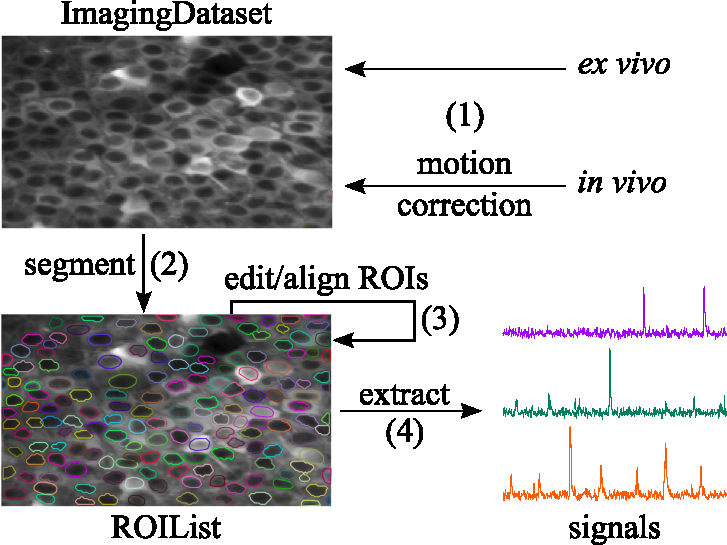
\includegraphics[width=0.7\textwidth]{sima/sima-fig1.pdf}
\caption[Workflow supported by SIMA]{
 Workflow supported by SIMA. 
 (1) An ImagingDataset object is first created either directly from the raw data
 or from the output of the motion correction algorithm.
 (2) ROIs are generated by automatic segmentation.
 (3) The ROI Buddy GUI can be used to edit the automatically generated ROIs and to
 automatically register ROIs across multiple datasets.
 (4) Dynamic fluorescence signals are extracted from the imaging data and ROIs.}
 \label{fig:sima:workflow}
\end{figure}

With just a few lines of code, the user can correct motion artifacts in the data,
and then segment the resulting \verb|ImagingDataset| object to identify 
ROIs:
\begin{verbatim}
dataset = sima.motion.hmm([[channel_A, channel_B]], '/save/path.sima')
dataset.segment()
\end{verbatim}
If the data lack motion artifacts (e.g.\ fluorescence imaging in \textit{ex vivo} brain slices), 
the motion correction step can be replaced with direct initialization of an
\verb|ImagingDataset| object.
The full set of commands in this case is an follows:
\begin{verbatim}
dataset = sima.ImagingDataset([[channel_A, channel_B]], '/save/path.sima')
dataset.segment()
\end{verbatim}
In either case, the result of these commands is an \verb|ImagingDataset| object
containing the raw or motion-corrected imaging data and the automatically
generated ROIs.
This object is permanently stored in the location \verb|/save/path.sima|
so that it can be reloaded at a later time.

Following automated segmentation, the generated ROIs can be manually edited with the ROI Buddy graphical user interface (GUI).
This GUI can be used to delete erroneous ROIs, add missing ROIs, merge ROIs that have been incorrectly split, and adjust the shapes and positions of existing ROIs.
The ROI Buddy GUI can also be used to register ROIs across multiple datasets acquired at different times, 
allowing for assessment of long-term changes in neural activity.

Once the ROIs have been edited and registered,
the \verb|ImagingDataset| object can be loaded in Python again,
and then dynamic fluorescence signals can be extracted from the ROIs as follows:
\begin{verbatim}
dataset = sima.ImagingDataset.load('/save/path.sima')
dataset.extract()
\end{verbatim}
The extracted signals are permanently saved with the \verb|ImagingDataset| object and can be accessed at any time with the command \verb|dataset.signals()|.
For further analysis with external software, the signals can be exported using the command \verb|dataset.export_signals('/export/path.csv')|.

The remainder of this section contains more detailed discussion of each of the 
stages of this workflow.
This discussion complements the API documentation that is available online at the project's website: \verb|http://www.losonczylab.org/sima|.


\subsection{Object classes and input formats}\label{sec:sima:inputs}
The SIMA package follows an object-oriented design.
The central object class around which the package is structured is the \verb|ImagingDataset|.
Objects of this class can be created either by direct initialization
or as the output of the motion correction function call.
Direct initialization of an \verb|ImagingDataset| object requires two mandatory arguments:
(1) the raw imaging data formatted according to the requirements discussed below, 
and (2) the path where the \verb|ImagingDataset| object is to be saved.
Names for the channels may be specified as an optional argument.
Once created, \verb|ImagingDataset| objects are automatically saved to the
designated location and can be loaded at a later time with
a call to the \verb|ImagingDataset.load| method.

A single \verb|ImagingDataset| object can contain imaging data from multiple
simultaneously recorded optical channels, as well as from multiple \textit{cycles} 
(i.e. continuous imaging epochs/trials) acquired at the same imaging location
during the same imaging session.
To allow for this flexibility, the raw imaging data used to initialize the
\verb|ImagingDataset| object must be packaged into a list of lists,
whose first index runs over the cycles and whose second index runs over the
channels.
For example, if the raw data is stored in an object called \verb|data|,
then the element \verb|data[i][j]| corresponds to the \verb|j|th channel of the
\verb|i|th cycle.

The formating requirements for each such element of the aforementioned list of lists
are designed to allow for flexible use of SIMA with
a variety of data formats.
The sole requirement is that each element be specified as a Python iterable
object satisfying the following properties: 
(1) the iterable may not be its own iterator, i.e. it should be able to spawn
multiple iterators that can be iterated over independently;
(2) each iterator spawned from the iterable must yield image frames in the form
of two-dimensional NumPy arrays;
and (3) the iterable must survive Python's pickling and unpickling methods
for saving and loading objects.

A simple example of an object that satisfies these requirements is a three-dimensional NumPy array,
with the first index corresponding to the frame, the second to the row, and the third to the column. 
Therefore, data in any format can be analyzed with SIMA following conversion
to a NumPy array.
We also implemented the \verb|sima.iterables.MultiPageTIFF| object class
for creating SIMA-compatible iterables from multi-page TIFF files,
and the \verb|sima.iterables.HDF5| object class for creating iterables from HDF5 files.
For example, a two-channel dataset can be initialized from TIFF files as follows:
\begin{verbatim}
iterables = [[sima.iterables.MultiPageTIFF('channel1.tif'),
              sima.iterables.MultiPageTIFF('channel2.tif')]]
dataset = sima.ImagingDataset(iterables, '/save/path.sima',
                              channel_names=['GCaMP', 'tdTomato'])
\end{verbatim}
Compared to converting data from TIFF or HDF5 files to NumPy arrays,
use of these custom iterables is advantageous because there is no need to
duplicate the data for separate storage in a second format.
Furthermore, less data need be held in memory at any one time because the
\verb|MultiPageTIFF| or  \verb|HDF5| iterables allow for imaging data
to be loaded one frame at a time on an as-needed basis.

Importantly, the SIMA package has been designed to allow for flexible extension
with additional custom iterable classes analogous to the \verb|MultiPageTIFF| class.
Such extensions can be developed to allow SIMA to use data from any required
input format.
Therefore, users wishing to use SIMA with other data formats have two options:
(1) to convert the data to a format already supported such as a TIFF stack or NumPy array,
or (2) to extend SIMA by creating a new iterable type to support the desired
data format.

\subsection{Motion correction}
During \textit{in vivo} laser-scanning microscopy, the animal's movements cause 
time-dependent displacements of the imaged brain region relative to the microscope and 
thus introduce substantial artifacts into the imaging data.
These artifacts are especially problematic when attempting to extract transient fluorescence 
signals from very small structures, such as dendritic branches and synaptic boutons (e.g.\ \citep{Kaifosh2013}).
Since individual pixels are acquired at different times during laser scanning microscopy,
motion artifacts can occur within a single frame and cannot be corrected by simple frame 
alignment methods.
To allow for correction of these within-frame motion artifacts, 
the SIMA package includes line-by-line motion correction software (igure \ref{fig:sima:motion})
that we developed \citep{Kaifosh2013}
by extending upon the hidden Markov model (HMM) approach used previously \citep{Dombeck2007}.

\begin{figure}[hb!]
\centering
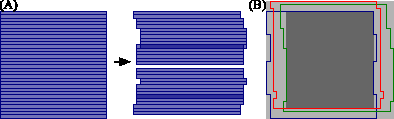
\includegraphics[width=0.7\textwidth]{sima/motion-correction.pdf}
\caption[Line-by-line correction of within-frame motion artifacts]{
 	Line-by-line correction of within-frame motion artifacts.
 	\textbf{(A)} Schematic diagram showing a single imaging frame before (left) and after (right)  line-by-line motion correction. 
	A separate displacement is calculated for each sequentially acquired line from the laser scanning process. As a result, some pixel locations may be accounted for multiple times (darker blue), while others may not be imaged in a given frame (white gap).
	\textbf{(B)} Overlay of different regions imaged by different frames due to motion. The light gray region indicates the maximum frame-size that can be selected for the motion correction output, such that all pixels locations that were ever imaged are within the frame. The dark gray region indicates the default and minimum frame-size that can be selected for the motion correction output, such that all pixels locations within the frame are within the field of view at all times.
 	}
 	\label{fig:sima:motion}
\end{figure}

A call to the hidden Markov model motion correction function \verb|sima.motion.hmm| returns a
motion-corrected \verb|ImagingDataset| object.
This function takes the same arguments used to directly initialize an
\verb|ImagingDataset| object, as well as additional arguments for specifying
parameters for the motion correction procedure.
One optional argument allows for specification of the number of states retained 
at each step of the Viterbi algorithm (see Section \ref{sec:sima:viterbi} for details).
Retaining a larger number of states may in some cases result in more accurate
displacement estimates, though at the expense of longer run-times.
The maximum allowable displacement in the horizontal and vertical directions 
can also be specified. 
Use of this restriction can improve the quality of the estimated displacements
by ruling out unreasonably large estimates.
Optionally, a subset of the channels can be selected for use in estimating
the displacements, which will then be used to correct artifacts in all channels.
This option is useful in cases where there is a sparse or highly dynamic channel with
signals of interest, and an additional static channel providing a stable
reference for motion correction.

Once the motion artifacts are corrected, the frames of the resulting \verb|ImagingDataset| show static
imaged structures, but a field of view that moves from frame to frame (Figure \ref{fig:sima:motion}B).
Typically, a frame size larger than that of the original images is required to display
the full spatial extent that was imaged during the session.
Relatedly, the area imaged during all frames is smaller than that of the original
images.
To determine the spatial extent of the corrected image series that will be
retained for further analysis, the \verb|hmm| function takes an additional
optional argument, 
the \verb|trim_criterion|, which specifies the fraction of frames for which
a location must be within the field of view in order to be retained for further
analysis.
By default, the edges of the corrected images are conservatively trimmed to retain
only the rectangular region that remains within the field of view during all imaging frames.


\subsection{Segmentation and ROIs}\label{sec:sima:ROIs}
The SIMA package allows for automated segmentation of the field of view with a call to the \verb|ImagingDataset.segment|
method.
The \verb|segment| method takes arguments that allow for specification of the approach
to be used and an optional label for the resulting set of ROIs, which are saved
with the \verb|ImagingDataset|.
Arguments specific to the particular method can also be passed into this
method call.
The SIMA package currently contains two implemented segmentation methods,
\verb|'normcut'| and \verb|'ca1pc'|, 
both of which are based on the normalized cuts approach \citep{Shi2000}.
Further details on these particular segmentation approaches are provided in Section \ref{sec:sima:details:segment}.

A call to the \verb|segment| method returns an \verb|ROIList| object,
which contains the segmented \verb|ROI| objects.
As well, \verb|ROI| objects can be initialized independently in one of four ways: 
(1) with a mask, typically a NumPy array, indicating the weight of each pixel (see Section \ref{sec:sima:details:extraction}),
(2) with a list of polygons, each consisting of a list of vertices,
(3) using ROI Buddy (see Section \ref{sec:sima:ROIbuddy}), or
(4) by importing a set of ROIs created in ImageJ \citep{schneider2012nih}.
Masks can either be binary, to select a subset of pixels, or real-valued, as in the case of
weights resulting from principal or independent component analysis.
Polygons are treated equivalently to binary masks.
ROIs typically consist of a single polygon, however multiple polygons are useful
for marking structures that leave and re-enter the imaging plane.

Additionally \verb|ROI| objects have the following
optional attributes: \verb|id|, \verb|label|, and \verb|tags|.
The \verb|label| attribute is a descriptor for the \verb|ROI| used for
referencing the region within one imaging session.
The \verb|id| of an \verb|ROI| object is an identifier used to track the region over
multiple imaging sessions, such that two \verb|ROI| objects from different experiments
that have the same \verb|id| are understood to correspond to the same neuron/dendrite/bouton.
The \verb|id| values are automatically set during ROI registration with the ROI Buddy GUI.
The \verb|tags| attribute is a set of strings associated with the \verb|ROI|, used for
sorting or marking the ROIs based on morphological, genetic, or other criteria.
These \verb|tags| can also be modified from within the ROI Buddy GUI or during analysis of fluorescence signals
to aid in the selection and sorting of ROIs during subsequent analysis.


\subsection{Manual ROI Editing}\label{sec:sima:ROIbuddy}
The ROI Buddy GUI can be used to view and edit the automated segmentation results
or to manually draw new ROIs.
When the user loads an \verb|ImagingDataset| object, the time-averaged images are displayed as a static background on which \verb|ROI|
objects are displayed.
The underlying static image can be toggled between each of the imaged channels,
and optionally a contrast-enhanced ``processed'' image can be displayed.
Each \verb|ROI| object, consisting of one or more polygons, is displayed with a unique color over this background.
If multiple \verb|ROIList| objects are associated with an \verb|ImagingDataset| 
(automatically generated and manually edited sets, for example), 
the active set is selectable via a drop-down menu.
The user can also toggle between simultaneously loaded \verb|ImagingDataset| objects, 
which is useful for rapidly switching between multiple imaging sessions of the same field of view
in order to verify the ROIs during editing.

% \begin{figure}
% \includegraphics[width=\textwidth]{/lab-admin/Presentations/figures/segmentation/ROI_Buddy_Figure.pdf}
% \caption[The ROI Buddy graphical user interface]{\label{fig:gui}
%  The ROI Buddy graphical user interface.
%  \textbf{(A)} Image viewing panel with ROI editing tools. During typical use this
%  			  panel is expanded to occupy the majority of the screen.
%  \textbf{(B)} Panel for toggling between ``Edit'' and ``Align'' modes,
%  			  loading imaging datasets, and registering ROIs across datasets.
%  \textbf{(C)} Panel for selecting, creating, saving, and deleting sets of ROIs associated
%  			  with the active imaging dataset. In ``Align'' mode, ROIs from all loaded
%  			  datasets can be viewed simultaneously.
%  \textbf{(D)} List of ROIs in the currently selected set, and
%  			  tools for tagging, merging, unmerging, and re-coloring ROIs.
%  \textbf{(E)} Contrast adjustment for the underlying base image.
%  \textbf{(F)} Panel for selection of the underlying base image.
%  }
% \end{figure}

Once the \verb|ImagingDataset| and \verb|ROI| objects are loaded in the GUI,
the user can edit, delete, and add new ROIs as polygons while in the GUI's ``Edit'' mode.
All ROIs are directly editable, allowing for the user to adjust individual vertices or translate the entire ROI.
In addition, separate polygons can be merged either into a single
multiple-polygon \verb|ROI| or, if the polygons are overlapping, into a single polygon \verb|ROI|.
The interface also allows the user to directly set the \verb|label| and \verb|tags|
properties of each \verb|ROI| described in Section \ref{sec:sima:ROIs}.


\subsection{ROI Registration}
To track the same structures over multiple imaging sessions of the same field of view (Figure \ref{fig:sima:registration}),
the ROI Buddy GUI also supports the registration of ROIs from different \verb|ImagingDataset| objects.
In the GUI's ``Align'' mode, affine transformations are estimated to align the time-averaged images
of the currently active \verb|ImagingDataset| with each of the other loaded sets.
These transformations are then applied to the respective \verb|ROI| objects to transform them all into the space of the active \verb|ImagingDataset| (Figure \ref{fig:sima:registration}C).
This allows ROIs to be imported from one set on to the active \verb|ImagingDataset| or for
all of the ROIs to be viewed simultaneously over the time-averaged image of a single \verb|ImagingDataset|.
The ROIs are then automatically identified across imaging datasets based on their degree of overlap
following transformation.  The \verb|id| attributes of co-registered \verb|ROI| objects are set to be equal,
thus allowing for tracking of the same regions over multiple imaging sessions.

When displayed in the GUI, 
co-registered \verb|ROI| objects are colored identically for easy visual 
inspection of the registration results (Figure \ref{fig:sima:registration}D).
Groups of co-registered ROIs can be manually modified by removing and adding \verb|ROI| objects
to correct any errors in the automated registration.
The \verb|tags| can also be propagated across co-registered ROIs from different \verb|ImagingDataset| objects.

\begin{figure}[]
	\centering
	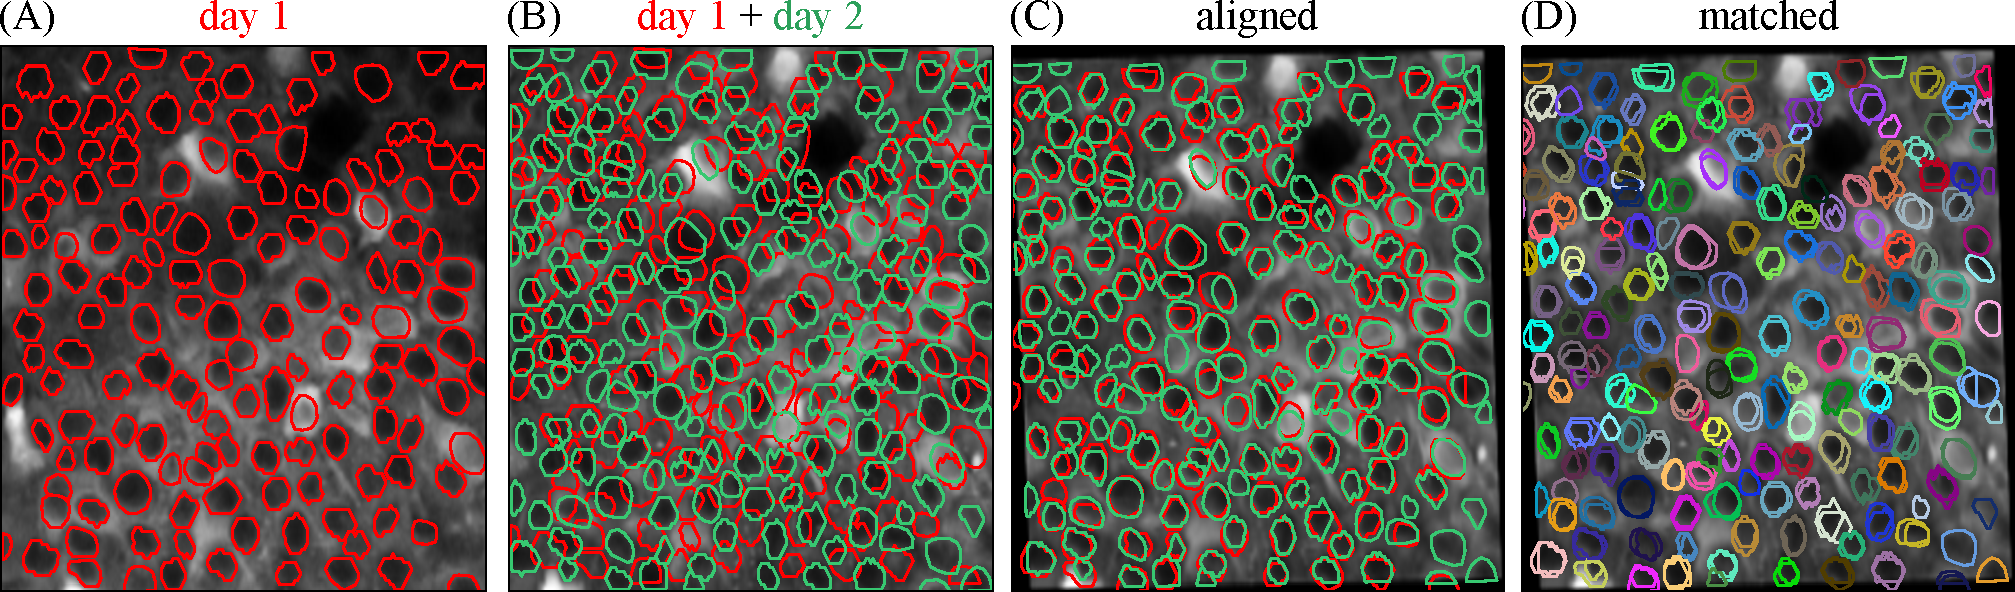
\includegraphics[width=0.9\textwidth]{sima/roi_registration-paper2.pdf}
	\caption[Registration of ROIs across imaging sessions acquired on two different days]{Registration of ROIs across imaging sessions acquired on two different days.
	\textbf{(A)} ROIs (red) and time-averaged image for the first imaging session.
	\textbf{(B)} ROIs (green) and time-averaged image for the second imaging session, with ROIs for the first imaging session (red) shown for comparison.
	\textbf{(C)} Same as \textbf{(B)} but with an affine transformation applied to align the time-averaged image and ROIs from day 2 to those of day 1.
	\textbf{(D)} Same as \textbf{(C)} but with the ROIs colored by their automatically determined shared identities across both imaging sessions.}
	\label{fig:sima:registration}
\end{figure}

\subsection{Signal extraction}
Signal extraction is accomplished by the \verb|ImagingDataset.extract| method.
This \verb|extract| method can take several optional arguments.
The \verb|ROIList| to be used can be specified in cases where there are multiple
\verb|ROIList| objects (e.g.\ one that has an automatically generated and another
that has been manually edited) associated with the \verb|ImagingDataset|.
If multiple optical channels are present, the channel to be used for extraction can be
specified.
If the ROIs are either polygons or a binary masks, 
the \verb|extract| method can optionally exclude pixels that overlap between ROIs in 
order to reduce artifactual correlations between adjacent ROIs.

The output of the \verb|extract| method is a Python dictionary, which is
also automatically saved as part of the \verb|ImagingDataset| object.
This dictionary contains
(1) the raw extracted signals, 
(2) a time-averaged image of the extracted channel,
(3) a list of the overlapping pixels,
(4) a record of which \verb|ROIList| and channel were used for extraction, and
(5) a timestamp.
Additionally, a verification image is saved as a PDF file showing the extracted ROIs
and overlapping pixels overlaid on the time-averaged image.
Once the signals are extracted, they can be accessed at any time with a call to the
\verb|ImagingDataset.signals| method.

\subsection{Exporting data}
The SIMA package is intended to provide support for early stages of data analysis,
such that subsequent analysis of the extracted signals can be performed with separate software.
In cases where all analysis is performed using Python, no exporting is necessary,
since the SIMA objects can be used in conjunction with other Python code.
In other cases, data from SIMA objects can be easily exported into standard formats,
including TIFF images and CSV text files.

Such exporting of data can be performed at various stages of data processing
with the SIMA package.
For example, those wishing to use SIMA solely for motion correction can export the
motion-corrected time series with a call to the \verb|ImagingDataset.export_frames| method.
This method takes as its argument the filenames with which the exported data
will be saved,
formatted as a list of lists of strings organized similarly to the input data
(see Section \ref{sec:sima:inputs}).
Additional optional arguments can be used to specify the output file format,
whether to scale the intensity values to the full range allowed by the output file format,
and whether to fill in unobserved rows (Figure \ref{fig:sima:motion}A) of motion corrected images with values
from adjacent frames.
Time-averaged images can similarly be exported with the \verb|ImagingDataset.export_averages|
method.

If SIMA is also used for signal extraction, then the extracted signals can be
exported to a CSV file with the \verb|ImagingDataset.export_signals| method.
The resulting CSV file contains the \verb|id|, \verb|label|, and \verb|tags| for each
ROI, and the extracted signal from each ROI at each frame time.


\section{Software details}\label{sec:sima:details}

% \subsection{Motion correction}

% We have previously described the HMM formulation and
% parameter estimation procedures that we have implemented for correction of within-plane
% motion during laser scanning microscopy \citep{Kaifosh2013}.
% Here we provide some additional details about the software implementation.


% \subsubsection*{Viterbi-based algorithm}\label{sec:sima:viterbi}
% The Viterbi algorithm computes the maximum \textit{a posteriori} sequence of states for a HMM.
% For a general HMM with $S$ hidden states and $T$ timesteps, the Viterbi algorithm has time complexity $O(S^2T)$.
% When used for motion correction, the hidden states are the possible displacements,
% with one state per pair of $x$ and $y$ integer displacements in pixel units.
% By restricting state transitions to those between nearest neighbors in two dimensions, 
% we reduce the complexity of the algorithm implemented in SIMA to $O(ST)$.
% This restriction is justified by the same assumption 
% -- that negligible motion occurs during the time required to image a row --
% by which we justify applying the same displacement to all pixels in the same row.
% Some of the datasets from our laboratory exhibit substantial displacements 
% in two dimensions, resulting in the number of states $S$ being rather large; 
% however, at any one time-step, the probability is typically concentrated in a much smaller number of states.
% Our software exploits this concentration of probability by retaining only the $N\ll S$ most probable states at each time-step.
% This approximation of the Viterbi algorithm reduces the computational complexity to $O(NT)$.

% Further increases in speed have been achieved by storing precomputed results for a number 
% of transformations applied to the reference image and the image being aligned.
% These transformations include scaling by the estimated gain factor (see \citep{Kaifosh2013}) to convert intensity values to estimated photon counts, 
% and computation of the logarithm and gamma functions applied to these scaled values.
% Repeated computations have also been avoided by using lookup tables for the indices
% of overlapping pixels between the image and the reference frame,
% for the possible transitions between hidden states,
% and for the probabilities of the transitions.


% \subsection{Segmentation}\label{sec:sima:details:segment}

% Although SIMA is designed to be extended to allow for multiple approaches to segmentation,
% the initial release includes only two segmentation methods, 
% both using the normalized cuts approach \citep{Shi2000}.
% Specifically, we have implemented a basic normalized cuts segmentation (\verb|'normcut'|),
% as well as a variant designed for segmentation of  pyramidal cell nuclei in hippocampal area CA1 (\verb|'ca1pc'|).
% Here, we describe first how we use the normalized cuts approach to partition the
% field of view, and then how, in the case of the \verb|'ca1pc'| variant, these regions
% are post-processed to create ROIs.

% \subsubsection{Normalized cut formation}
% The normalized cut segmentation algorithm \citep{Shi2000} partitions the imaged field
% of view through an iterative process.
% At each stage, a subset of the image pixels is split into two new subsets in such 
% a way as to minimize a penalty that depends on a set of connection weights between the pixels.
% The resulting normalized cuts are uniquely determined by two factors: 
% (1) the connection weights between pixels, and (2)
% the termination criterion for the iterative splitting procedure.

% For the standard normalized cuts procedure implemented in SIMA,
% the weight $w_{ij}$ between each pair of pixels $i$ and $j$ is calculated as follows:
% \begin{equation}\label{eq:weights}
%   w_{ij} = e^{k_cc_{ij}} \cdot
%   \begin{cases}
%    e^{-\frac{||\mathbf x_i- \mathbf x_j||^2}{\sigma_{\mathbf x}^2}} 
%       & \text{if }||\mathbf x_i - \mathbf x_j|| < r\\
%     0 & \text{otherwise}
%   \end{cases},
% \end{equation}
% where $c_{ij}$ is an estimate of the correlation between the pixels' intensity signals,
% $||\mathbf x_i - \mathbf x_j||$ is the Euclidean distance between the
% positions $\mathbf x_i, \mathbf x_j$ of the pixels,
% and $\sigma_{\mathbf x}^2$ specifies the decay of weights with distance 
% up to a maximum distance $r$. 
% We set the parameter $k_c=9$ based on empirical observations of segmentation accuracy.

% For the \verb|'ca1pc'| variant, we use a different set of weights $w_{ij}^{\text{CA1PC}}$,
% which are calculated by multiplying the weights $w_{ij}$ from Equation \eqref{eq:weights}
% by a factor depending on the maximum pixel intensity along a line connecting the two pixels.
% Specifically, the modified weights are defined as
% \begin{equation}
%  w_{ij}^{\text{CA1PC}} = 
%  w_{ij}\cdot
%  \exp\left(-k_I\max_{s\in[0,1]} I_{\text{avg}}^*\left((1-s)\mathbf x_i + s\mathbf x_j\right)\right),
% \end{equation}
% where $I_{\text{avg}}^*(\mathbf x)$ is the intensity at location $\mathbf x$ 
% of the time-averaged image, processed with Contrast Limited Adaptive Histogram Equalization (CLAHE) and an unsharp mask
% in order to correct intensity inhomogeneities and enhance the contrast
% (Figure \ref{fig:segmentation}B).
% Based on empirical observations of segmentation accuracy,
% we set $k_I = 3 / (\max I_{\text{avg}}^* - \min I_{\text{avg}}^*)$,
% with the maximum and minimum taken over the entire image.
% The effect of this modification is to increase the weights between two pixels 
% within the same low-intensity pyramidal cell nucleus relative to the weights between other
% pixels.

% \begin{figure}
% \includegraphics[width=\textwidth]{/lab-admin/Presentations/figures/sima/processing_steps.pdf}
%  \cprotect\caption[Segmentation steps for identifying pyramidal cell nuclei with the \verb|'ca1pc'| variant of the normalized cuts segmentation approach]{\label{fig:segmentation}
%   Segmentation steps for identifying pyramidal cell nuclei with the \verb|'ca1pc'| variant of the normalized cuts segmentation approach.
%   \textbf{(A)} The time-averaged image of the time-series to be segmented.
%   \textbf{(B)} Application of CLAHE and unsharp mask image processing to \textbf{(A)}.
%   \textbf{(C)} Disjoint regions identified by iterative partitioning with the normalized cuts algorithm.
%   \textbf{(D)} Local Otsu thresholding of each region in \textbf{(C)}.
%   \textbf{(E)} Cleanup of the Otsu thresholded regions in \textbf{(D)} with opening and closing binary morphology operations.
%   \textbf{(F)} Resulting ROIs after rejection of regions in \textbf{(E)} that failed
%                to satisfy minimum size and circularity requirements.
%  }
% \end{figure}

% The termination criterion for the iterative partitioning of the image
% depends on the number of pixels in the region and
% the normalized cut penalty for the next potential partitioning. 
% Specifically, partitions containing fewer than a minimum number of pixels (\verb|cut_min_size|)
% do not undergo further partitioning,
% whereas partitions with greater than a maximum of pixels (\verb|cut_max_size|) always 
% undergo further partitioning.
% For partitions with an intermediate number of pixels, further partitioning
% occurs only if the penalty associated with the partitioning would be below
% a given threshold.
% For populations of uniformly sized neurons, such as those in the pyramidal 
% layer of CA1, suitable termination is achieved when the values for \verb|cut_max_size| and \verb|cut_min_size| are chosen
% as upper and lower bounds on the typical cell size.
% An example set of partitions obtained with the \verb|'ca1pc'| variant
% is shown in Figure \ref{fig:segmentation}C.

% \subsubsection{Post-processing of partitions}
% In contrast to the basic \verb|'normcut'| segmentation method,
% which simply returns the partitions as the ROIs,
% the \verb|'ca1pc'| variant applies a series of post-processing
% steps to these partitions to isolate the darker pixels corresponding
% to the putative CA1 pyramidal cell nuclei.
% First a threshold is calculated for each partition based on Otsu's method 
% \citep{Otsu1979} for 
% cluster-based thresholding, allowing for the rough separation of light and dark pixels
% (Figure \ref{fig:segmentation}D).
% Following this step a series of morphological operations,
% consisting of a binary opening followed by a binary closing,
% are applied to each identified region to regularize the ROI shapes by
% filling in gaps and smoothing the borders of each region (Figure \ref{fig:segmentation}E).
% Finally a minimum size and circularity criterion is applied to each region to
% reject small and irregularly shaped regions (Figure \ref{fig:segmentation}F).

% We evaluated this \verb|'ca1pc'| segmentation algorithm on two-photon fluorescence imaging data
% from GCaMP6f-expressing pyramidal cells in hippocampal area CA1 
% (see \citep{Lovett-Barron2014} for methodological details).
% Each of the 37 datasets consisted of 4575 frames of size 128x256 pixels acquired at 7.6 Hz
% with a 40x Nikon immersion objective at optical zoom 2X.
% We ran the segmentation algorithm with the following parameters: 
% \verb|num_pcs| = \verb|50|, 
% \verb|max_dist| = \verb|(3, 6)|,
% \verb|spatial_decay| = \verb|(3, 6)|,
% \verb|cut_max_pen| = \verb|0.10|,
% \verb|cut_min_size| = \verb|50|,
% \verb|cut_max_size| = \verb|150|,
% \verb|x_diameter| = \verb|14|,
% \verb|y_diameter| = \verb|7|,
% \verb|min_roi_size| = \verb|20|,
% \verb|circularity_threhold| = \verb|.5|,
% and \verb|min_cut_size| = \verb|40|.
% We compared the automatically segmented ROIs with manually curated segmentation.
% With a minimum Jaccard index of 0.25 as the criterion for a match between ROIs,
% the automatic segmentation had a false negative rate of 12$\pm$2\% and a false positive rate of
% 20$\pm$5\% (mean $\pm$ standard deviation).


\subsection{ROI Registration}
To estimate affine transformations between pairs of time-averaged images, we used the function
\verb|getAffineTransform| from OpenCV.
Once ROIs are transformed into the same reference space, the ROI Buddy GUI can automatically estimate
the degree of similarity between each pair of ROIs from different \verb|ImagingDataset| objects by calculating the Jaccard index,
defined as the area of the intersection divided by the area of the union.
ROIs are then clustered with the unweighted pair group method with arithmetic mean (UPGMA) hierarchical
clustering algorithm \citep{Sokal1958}, with distances between ROIs given by the reciprocal of the Jaccard index for that pair.
ROI pairs from the same \verb|ImagingDataset| are assigned infinite distance to prevent co-clustering of ROIs from the same imaging session. 
The termination criterion for clustering is set such that pairs of ROIs in a cluster have a minimum Jaccard index of 0.25.
The objects of each cluster are then assigned a common \verb|id| attribute, allowing for identification
of the same region over multiple imaging sessions.


\subsection{Signal extraction}\label{sec:sima:details:extraction}
In discussing the extraction procedures, 
we use the notation $w_{ip}$ to denote the weighting of the $p$th pixel by the $i$th ROI.
For polygon or binary mask ROIs, 
created with SIMA's automated segmentation or the ROI Buddy GUI, or imported from ImageJ,
$w_{ip}$ is defined as $\frac{1}{N_i}$ for pixels $p$ within the ROI and 0 elsewhere, where $N_i$ is the
number of pixels in the $i$th ROI.

The simplest case for extraction occurs when the same pixel locations are imaged in every frame.
In this case, we calculate the signal by a simple weighting of the normalized fluorescence intensities
from each pixel.
Specifically, the signal of the $ith$ ROI at time $t$ is calculated as
\begin{equation}\label{eq:extraction-basic}
    s_{it} = \sum_p w_{ip}\cdot \frac{f_{pt}}{f_p},
\end{equation}
with $f_{pt}$ denoting the intensity of the $p$th pixel in the frame at time $t$,
and $f_p$ denoting the average intensity across all frames at pixel location $p$.

When extracting signals following correction of within-frame motion artifacts,
the situation is complicated by the fact that not all pixel locations are observed
in each frame.
To derive a method for extracting these signals, we first note that the simple extraction method (equation \ref{eq:extraction-basic})
reduces to the least-squares error estimate for a simple linear model in which the 
pixel intensities are related to the underlying ROI signals as follows:
\begin{equation*}
    \frac{f_{pt}-f_p}{f_p} = \sum_i a_{pi} (s_{it} - s_i^*),
\end{equation*}
with the coefficients $a_{pi}$ defined as the entries of the pseudoinverse of the matrix with
entries given by the weights $w_{ip}$,
and with $s_i^*$ set as $\sum_p w_{ip}$.
Given this model, when a subset $P_t$ of the pixels are imaged in the frame taken at time $t$,
the least squares estimate of the signal is given by
\begin{equation*}
    s_{it} = \sum_{p} w_{ipt}\cdot \frac{f_{pt}-f_p}{f_p} + \sum_p w_{ip}.
\end{equation*}
Here, the time-dependent coefficients $w_{ipt}$ are defined as the entries of the pseudo-inverse
of the matrix with entries $a_{pi}$ for all pixels $p$ in $P_t$.

A few special cases are worth mentioning.
For non-overlapping ROIs, this formula reduces to
\begin{equation*}
    s_{it} = \frac{\sum_p w_{ip}^2}{\sum_{p\in P_t} w_{ip}^2}\cdot \sum_{p\in P_t} w_{ip}\frac{f_{pt}-f_p}{f_p} + \sum_p w_{ip}.
\end{equation*}
In cases of binary mask or polygon ROIs, the above formula simplifies to
\begin{equation*}
    s_{it} = \frac{1}{N_{it}}\cdot\sum_{p\in P_{it}}\frac{f_{pt}}{f_p},
\end{equation*}
where $P_{it}$ is the set of pixels in the $i$th ROI that were imaged at time $t$,
and $N_{it}$ the number of pixels in this set.
In cases in which no pixels of a given ROI are imaged in a given frame,
a not-a-number (\verb|numpy.NaN|) value is recorded in place of that ROI's signal at that time.

% \subsubsection{Signal demixing}
% In addition to the raw signal extraction, SIMA also contains the option to separate out
% different fluorophores that are mixed across multiple optical channels.
% In this case, we perform signal extraction not on the raw optical channels,
% but rather on linear combinations of the optical channels.
% To estimate the linear combinations required to isolate the fluorescence from
% individual fluorophores, we perform independent component analysis on the pixel
% intensities of the time-averaged images from each optical channel.


% \subsection{Requirements and Dependencies}
% The SIMA package and ROI Buddy GUI depend only upon freely available open source software.
% In particular, the NumPy and SciPy packages \citep{Oliphant2007,Jones2001} for numerical 
% and scientific computing are relied upon heavily throughout. 
% The extraction functionality uses Matplotlib \citep{Hunter2007} to generate 
% verification images.
% The Shapely Python package is used for geometric calculations relating to polygon ROIs.
% Automated segmentation relies upon Scikit-image \citep{Walt2014} and the Open Source 
% Computer Vision Library (OpenCV), the latter which is also used for ROI registration.
% The ROI Buddy user interface uses guiqwt (http://code.google.com/p/guiqwt/).
% HDF5 files are manipulated with the h5py interface (http://www.h5py.org/).
% These packages are available with a standard scientific Python installation.
% Since the libtiff C library and its Python bindings enable more memory-efficient 
% handling of multi-page TIFF files,
% their installation is strongly recommended if SIMA is to
% be used with large TIFF files containing many frames.

% \section{Discussion and Future Developments}\label{sec:sima:discussion}
% As a freely available open source software package, SIMA provides a variety of
% tools to facilitate common steps of dynamic fluorescence imaging analysis, 
% including correction of motion artifacts,
% segmentation of the field of view into ROIs,
% and extraction of the fluorescence time-series for each ROI.  
% Data can be imported or exported at various stages of processing with SIMA,
% so that the package can be used for all stages of analysis,
% or for any combination of the motion correction, segmentation, and signal extraction.
% The SIMA package can thus be used flexibly in conjunction with other analysis software.
% We have thoroughly documented the SIMA package to facilitate use and 
% future collaborative development of this open source project
% (project hosted on GitHub at https://github.com/losonczylab/sima).

% Some of the functionality contained in the SIMA package complements other existing 
% fluorescence imaging acquisition and
% analysis tools, such as Micro-Manager \citep{Edelstein2010} and ACQ4 \citep{Campagnola2014}.
% The TurboReg plug-in for ImageJ \citep{thevenaz1998pyramid}
% is capable of correcting motion artifacts that produce mis-aligned frames,
% but does not allow for correction of within-frame motion artifacts that occur during
% laser scanning microscopy.
% The normalized cuts approach to segmentation \citep{Shi2000} is a novel technique for the
% segmentation of dynamic fluorescence imaging data and is complementary to existing approaches,
% such as spatio-temporal independent complement analysis \citep{Mukamel2009},
% convolutional sparse block coding \citep{pachitariu2013extracting},
% and other methods implemented in ImageJ or CalTracer (\url{http://www.columbia.edu/cu/biology/faculty/yuste/methods.html}).
% In addition to providing this additional approach to segmentation, 
% we have also created a graphical user interface, ROI Buddy, 
% for manual editing of automatically generated ROIs,
% and for automated registration of ROIs across multiple datasets.
% ImageJ also provides the ability to draw ROIs and extract signals from image timeseries, but lacks the ability to handle missing data.
% Overall, a major advantage of SIMA is the integration of these various processing stages into a 
% single tool-kit, allowing for seamless execution of the early stages of analysis
% of time series laser-scanning microscopy data.

% We plan to extend the SIMA package, hopefully in collaboration with the
% neuroinformatics community, so that future versions have greater functionality.
% A major need is to extend SIMA with additional methods for automated segmentation.
% Since the optimal segmentation approach is dependent on the neural structures recorded,
% the imaging conditions, and the goals of the analysis, we have structured the SIMA module such that
% additional approaches can be easily implemented and applied to \verb|ImagingDataset| objects.
% Integration of other existing segmentation approaches into the SIMA package is an area of active development.

% A second avenue for future development is to generalize the applicability of the
% SIMA package to imaging data acquired by methods other than two-dimensional laser
% scanning microscopy.
% In particular, we are interested in extending SIMA to work with newer technologies
% allowing for three-dimensional imaging within a volume of neural tissue.
% Such technologies include temporal focusing \citep{schrodel2013brain}, 
% light sheet imaging \citep{verveer2007high}, light field imaging \citep{Levoy:2006:LFM:1141911.1141976},
% and resonance scanning in combination with a piezoelectric crystal.
% The extension of our software to these technologies should support their broader application.

% \section*{Supplemental Data}
% Extensive documentation for the SIMA package and ROI Buddy GUI
% is available at \url{http://www.losonczylab.org/sima/}.
% Software and source code can be downloaded from the Python Package Index: 
% \url{https://pypi.python.org/pypi/sima}.
% The source code repository is maintained on GitHub:
% \url{https://github.com/losonczylab/sima}.

\chapter{Other Applications}
\acresetall
\chapter{Other Applications}
\label{ch:other}

\section{Chronic remapping}\label{sec:applications:chronic}
\todo[inline, color=yellow]{Include chronic remapping results?}

\section[Gating of hippocampal activity, plasticity, and memory by entorhinal cortex long-range inhibition]{Gating of hippocampal activity, plasticity, and memory by entorhinal cortex long-range inhibition\footnote{This work has been previously published \citep{Basu2016} and is joint work with the coauthors.}}
\label{sec:other:LRIP}

\begin{quote}
The cortico-hippocampal circuit is critical for storage of associational memories. Most studies have focused on the role in memory storage of the excitatory projections from entorhinal cortex to hippocampus. However, entorhinal cortex also sends inhibitory projections, whose role in memory storage and cortico-hippocampal activity remains largely unexplored. We found that these long-range inhibitory projections enhance the specificity of contextual and object memory encoding. At the circuit level, these g-aminobutyric acid (GABA)–releasing projections target hippocampal inhibitory neurons and thus act as a disinhibitory gate that transiently promotes the excitation of hippocampal CA1 pyramidal neurons by suppressing feedforward inhibition. This enhances the ability of CA1 pyramidal neurons to fire synaptically evoked dendritic spikes and to generate a temporally precise form of heterosynaptic plasticity. Long-range inhibition from entorhinal cortex may thus increase the precision of hippocampal-based long-term memory associations by assessing the salience of mnemonic information to the immediate sensory input.
\attrib{\citealt{Basu2016}}
\end{quote}

This project was primarily the work of the first author, Jayeeta Basu, who performed the slice physiological recordings characterizing this long-range inhibitory projection (LRIP) from lateral entorhinal cortex (LEC) to the \emph{stratum lacunosum moleculare} of hippocampal area CA1, which gated a a specific form of input timing-dependent plasticity between CA3 Schaffer collaterals and CA1 pyramidal cells. In addition, Dr. Basu showed that interrupting this projection \emph{in vivo} affected both context and object recognition memory. As further evidence for the \emph{in vivo} role of these LRIPs from LEC to CA1, I imaged these fibers in CA1 while mice were running and exposed to various sensory stimuli.

We found that LEC inhibitory axons in CA1 showed robust responses to aversive (air puff), appetitive (water), and contextual (tone and light) stimuli. (\autoref{fig:other:LRIP:imaging}).
In addition, these responses were coherent across buttons on a single axons and individual boutons responded to more than 2 stimuli at a higher rate than chance, together suggesting that there is a subpopulation of LEC inhibitory projecting cells which preferentially encode contexts as a whole (\autoref{fig:other:LRIP:boutons}).

\begin{figure}
	\centering
	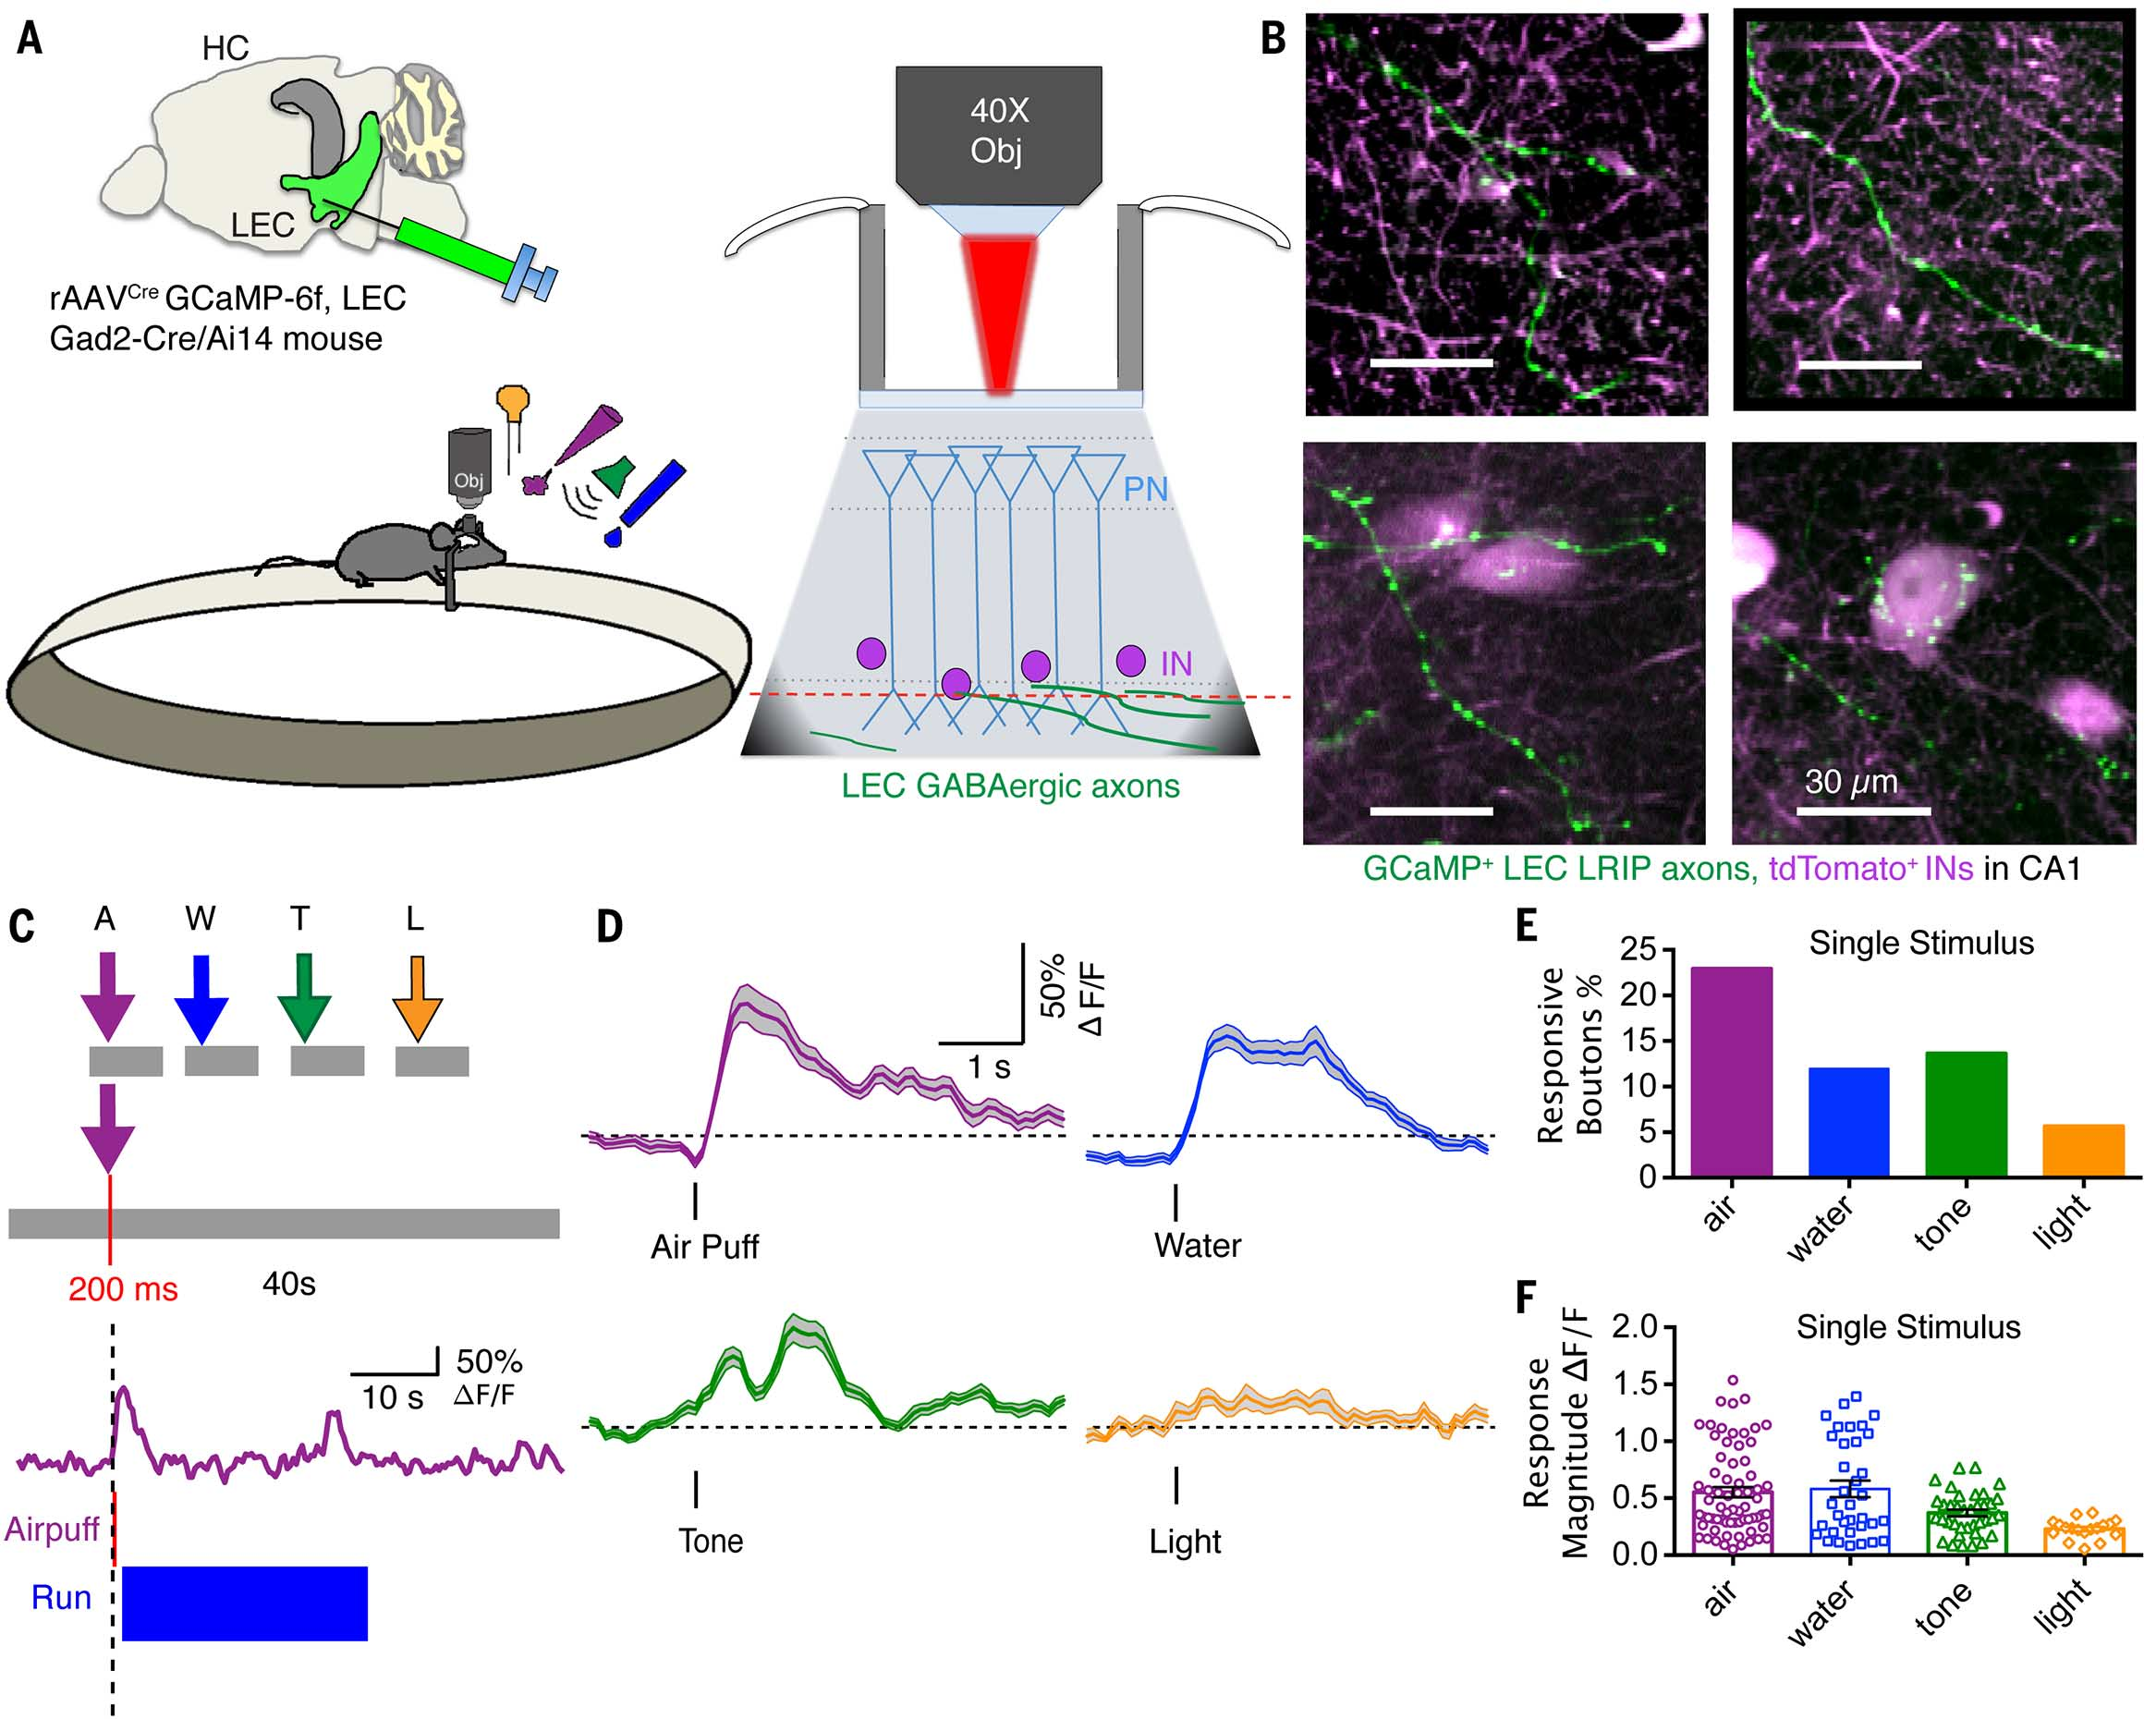
\includegraphics[width=0.75\textwidth]{applications/LRIP_Fig3_edit}
	\caption[Functional imaging of sensory coding in LEC LRIPs present in SLM of CA1]{Functional imaging of sensory coding in LEC LRIPs present in SLM of CA1.
	A) Diagram of in vivo imaging experiment. GCaMP6f was expressed in dorsal LEC, by injecting Cre-dependent rAAV in \emph{Gad2-Cre/Ai} 14 mice that also expressed tdTomato in all GABAergic neurons. A 40$\times$ water immersion objective was used for two-photon imaging through a cranial window over CA1 in head-fixed awake mice during multimodal sensory and behavioral stimuli presentation.
	(B) Four examples of time-averaged images of GCaMP6f fluorescence in LEC LRIP axons in SLM (green) with tdTomato labeling CA1 interneurons (magenta).
	(C) Experimental design of single-stimulus protocol. Imaging was performed in blocks of four trials, each 40 seconds in duration. After a 10~$\pm$~3~s baseline, one of four types of stimuli -- aversive air puff (A), water drop (W), tone (T), or light (L) -- was presented in random order for 200~ms, except the water drop was limited to 50~ms to prevent satiation. Each block was repeated to obtain at least five trials per stimulus. The animal's behavioral response (running and licking) was monitored. $\Delta F/F$ traces showing increased Ca\super{2+} signal in a single bouton on an LRIP axon in response to air puff.
	(D) Mean ($\pm$ SEM) $\Delta F/F$ Ca\super{2+} signal (PSTH) from responsive ROIs to indicated stimuli.
	(E) Percentage of responsive boutons to the stimuli (air~=~22.92\%, water~=~11.96\%, tone~=~13.64\%, and light~=~5.65\%).
	(F) Scatter and mean ($\pm$ SEM) plots of $\Delta F/F$ signals from individual responsive boutons (air~=~0.55~$\pm$~0.05, n~=~68; water~=~0.58~$\pm$~0.07, n~=~35; tone~=~0.37~$\pm$~0.03, n~=~37; light~=~0.23~$\pm$~0.02, n~=~18).
	% (G) Experimental protocol: Imaging was performed as described above, but in response to pairs of stimuli, presented in blocks of 10 trials, each 40 seconds long. Stimuli were randomized and paired stimuli were interleaved with single stimulus presentations.
	% (H) Mean ($\pm$ SEM) $\Delta F/F$ Ca\super{2+} signal (PSTH) from responsive ROIs to paired stimuli.
	% (I) Percentage of responsive boutons for paired stimuli (A+T~=~32.8\%; A+L~=~45.3\%; A+W~=~25.4\%; W+T~=~13.3\%; W+L~=~15.6\%; T+L~=~14.1\%).
	% (J) Scatter and mean ($\pm$ SEM) plots of $\Delta F/F$ signals to paired stimuli from individual responsive boutons (A+T~=~0.76~$\pm$~0.07, n~=~44; A+L~=~0.74~$\pm$~0.05, n~=~58; A+W~=~0.34~$\pm$~0.03, n~=~31; W+T~=~0.48~$\pm$~0.09, n~=~17; W+L~=~0.49~$\pm$~0.04; T+L~=~0.41~$\pm$~0.045, n~=~18).
	}
	\label{fig:other:LRIP:imaging}
\end{figure}

\begin{figure}
	\centering
	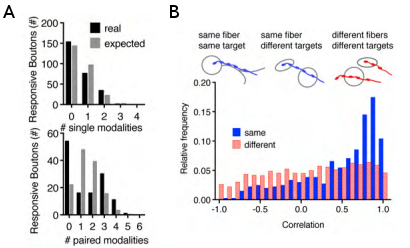
\includegraphics[width=0.75\textwidth]{applications/LRIP_FigS8_edit}
	\caption[Responsive properties of LRIP boutons]{Responsive properties of LRIP boutons. (A) Histogram bar plots of the number of responsive boutons (y axis) as a function of the number of stimulus modalities (x axis) to which a given bouton responds, either with a single sensory stimulus (above) or two stimuli presented simultaneously (below). The experimental data is plotted in black while the distribution expected if the stimuli and bouton responses were independent is in gray. For single stimulus presentations, very few boutons respond to more than one type of stimulus, following the predictions for independent responses (P~=~0.01659). In contrast, paired stimuli evoke Ca\super{2+} responses in a greater than expected number of boutons (P~$<$~0.03), perhaps the influence of a single overlapping stimulus in paired modalities (e.g. bouton responding to airpuff alone would likely respond to all three pairings with air; A+T, A+L, A+W).
	(B) Relative frequency distribution of bouton-bouton Ca\super{2+} response correlation coefficients for all identifiable bouton pairs originating from the same axon segment (solid blue, r~=~0.488 $\pm$ 0.017, n~=~808) versus boutons from different axons (cross-hatched red, r~=~0.115 $\pm$ 0.009, n~=~3992; P~$<$~0.0001, Mann-Whitney U test). Response similarity was determined by calculating the z-scored response magnitude for each stimulus for each bouton and then comparing the responses of pairs of boutons by calculating the correlation between their responses across all stimuli.
	}
	\label{fig:other:LRIP:boutons}
\end{figure}


\section[Distinct Contribution of Adult-Born Hippocampal Granule Cells to Context Encoding]{Distinct Contribution of Adult-Born Hippocampal Granule Cells to Context Encoding\footnote{This work has been previously published \citep{Danielson2016a} and is joint work with the coauthors.}}

% In brief, dentate gyrus granule cells are one of the few populations of neurons that undergoes continue neurogenesis in the adult mammalian brain.
\begin{quote}
Adult-born granule cells (abGCs) have been implicated in cognition and mood; however, it remains unknown how these cells behave in vivo. Here, we have used two-photon calcium imaging to monitor the activity of young abGCs in awake behaving mice. We find that young adult-born neurons fire at a higher rate in vivo but paradoxically exhibit less spatial tuning than their mature counterparts. When presented with different contexts, mature granule cells underwent robust remapping of their spatial representations, and the few spatially tuned adult-born cells remapped to a similar degree. We next used optogenetic silencing to confirm the direct involvement of abGCs in context encoding and discrimination, consistent with their proposed role in pattern separation. These results provide the first in vivo characterization of abGCs and reveal their participation in the encoding of novel information.
\attrib{\citealt{Danielson2016a}}
\end{quote}

While this project is the primary work of the first author, the behavioral apparatus, experimental paradigms, and analysis tools were all developed jointly.
In particular, this manuscript was Attila Losonczy's lab's first publication of head-fixed two-photon calcium imaging of place cells in mice, so relied upon upgrades to the behavioral apparatus (\autoref{sec:intro:techniques:behavior}), the imaging processing pipeline (\autoref{sec:intro:techniques:pipeline}), and analysis of place cell data (\autoref{sec:intro:techniques:place-cells}).

\begin{figure}
	\centering
	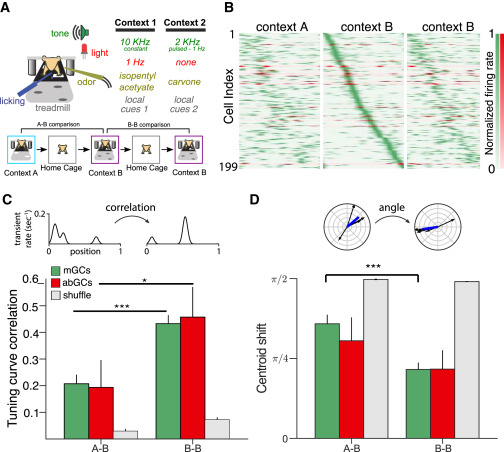
\includegraphics[width=0.8\textwidth]{applications/abGC_Fig3}
	\caption[Contextual coding by adult-born and mature granule cells]{Contextual coding by adult-born and mature granule cells.
	A) Experimental schematic. Mice ran for three 12-min sessions in contexts A, B, and B (1 hr between runs). A and B refer to either context 1 or 2 (chosen randomly for each experiment).
	(B) Remapping of spatial rate maps across sequential context exposures. Smoothed calcium transient rates, normalized to peak for each cell, are plotted as a function of position during three contextual exposures (A, B, B). Cells (mGCs, green; abGCs, red) are ordered according to the position of peak activity during the first exposure to context B. Data is shown for GCs with sufficient tuning specificity and activity (p~$<$~0.1, at least four transients) in at least one experiment.
	(C and D) Context specificity of spatial representations. Tuning curve correlations of 1D rate maps (C) and centroid shifts (angle between tuning directions) (D) between sequential exposures to different (A-B) or the same (B-B) contexts for all cells shown in (B) (A-B: n~=~180 mGCs, 14~abGCs; B-B: n~=~174 mGCs, 9~abGCs). The rate map correlations of both populations were more similar in the B-B condition than in A-B (Mann-Whitney U, mGCs: U(150)~=~5,291, p~$<$~0.001; abGCs: U(18)~=~23.0, p~$<$~0.05). In mGCs the tuning shift was larger in the A-B condition than in B-B, although this did not reach significance in abGCs (mGCs: U(150)~=~5,714, p~$<$~0.001; abGCs: U(18)~=~40.0, p~=~0.34). In both conditions, the similarity of spatial representations exceeded chance levels as estimated by shuffling cell identity (gray).
	Error bars are mean~$\pm$~SEM.}
	\label{fig:other:dg:context}
\end{figure}

\section[Sublayer-Specific Coding Dynamics during Spatial Navigation and Learning in Hippocampal Area CA1]{Sublayer-Specific Coding Dynamics during Spatial Navigation and Learning in Hippocampal Area CA1\footnote{This work has been previously published \citep{Danielson2016b} and is joint work with the coauthors.}}

\begin{quote}
The mammalian hippocampus is critical for spatial information processing and episodic memory. Its primary output cells, CA1 pyramidal cells (CA1 PCs), vary in genetics, morphology, connectivity, and electrophysiological properties. It is therefore possible that distinct CA1 PC subpopulations encode different features of the environment and differentially contribute to learning. To test this hypothesis, we optically monitored activity in deep and superficial CA1 PCs segregated along the radial axis of the mouse hippocampus and assessed the relationship between sublayer dynamics and learning. Superficial placemaps were more stable than deep during headfixed exploration. Deep maps, however, were preferentially stabilized during goal-oriented learning, and representation of the reward zone by deep cells predicted task performance. These findings demonstrate that superficial CA1 PCs provide a more stable map of an environment, while their counterparts in the deep sublayer provide a more flexible representation that is shaped by learning about salient features in the environment.
\attrib{\citealt{Danielson2016b}}
\end{quote}

This project was the primary work of the first author, Nathan Danielson, but again a lot of the experimental designs, tools, and procedures were developed collaboratively: \ac{GOL} task (\autoref{sec:intro:techniques:GOL}, \autoref{fig:other:sf-deep:GOL}), place cell stability metrics (\autoref{sec:intro:techniques:place-cells}, \autoref{fig:other:sf-deep:stability}), and reward enrichment analysis (\autoref{fig:other:sf-deep:enrichment}).

\begin{figure}
	\centering
	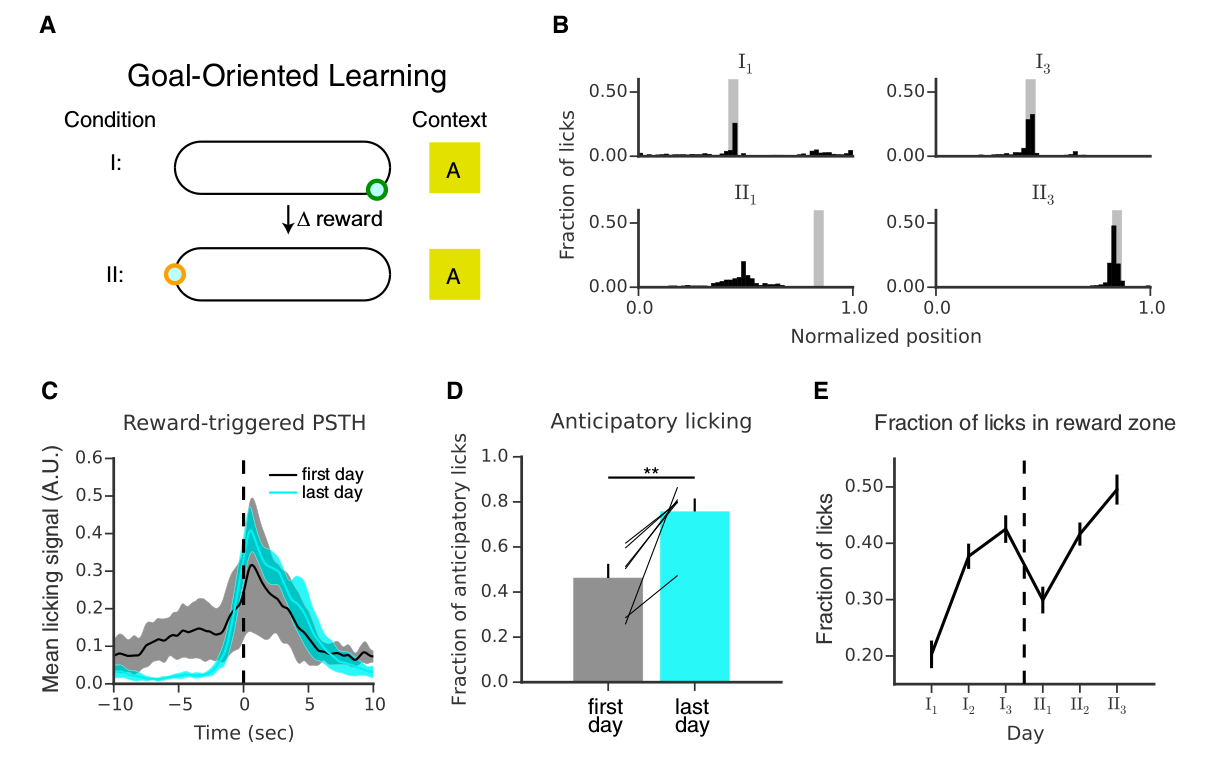
\includegraphics[width=0.8\textwidth]{applications/sf_deep_Fig3}
	\caption[GOL Task for Head-Fixed Imaging]{GOL Task for Head-Fixed Imaging.
	(A) Schematic of the goal-oriented learning (GOL) task. Mice (n~=~6) searched for an unmarked reward zone, and water rewards were administered only when the mice licked within the fixed 10-cm goal. At the end of condition I, the reward was moved to a new location of the belt, and the experiment was repeated (condition II). The same context (A) was maintained throughout.
	(B) Representative licking data from four individual experiments from one mouse performing the task. The fraction of total licks is plotted as a function of position on the belt (50 bins, 4 cm per bin). The reward zone is shaded gray. On the first day of the experiment, the mouse licked diffusely throughout the belt as it searched for the hidden reward zone. By the last day of condition I, the mouse licked selectively at the reward location. After the reward was moved, the mouse continued to lick at the original reward location. It eventually reverted to an exploratory licking state, and by the end of condition II the mouse selectively licked at the new reward location.
	(C) Peri-stimulus time histogram (PSTH) of licking rate triggered on reward zone entry for the first (black) and last (cyan) days of each condition. PSTHs were calculated for each mouse and smoothed with a 1-s Hamming filter. Shaded regions indicate mean $\pm$ SD across mice. Licking was initially diffuse. By the last day, licking outside the reward zone was largely suppressed and rose sharply prior to reward zone entry, reflecting the expectation of reward. The effect was highly consistent across mice.
	(D) Anticipatory licking (fraction of non-reward zone licks in the 10~cm preceding the reward) increased significantly by the end of learning (n~=~6 mice, p~$<$~0.01, paired t-test). Error bars indicate mean $\pm$ SEM across mice.
	(E) The fraction of licks occurring within the reward zone aggregated by recording session and plotted by day (mean $\pm$ SEM across mice). Over time, licking became more selective for the reward zone.
	}
	\label{fig:other:sf-deep:GOL}
\end{figure}

\begin{figure}
	\centering
	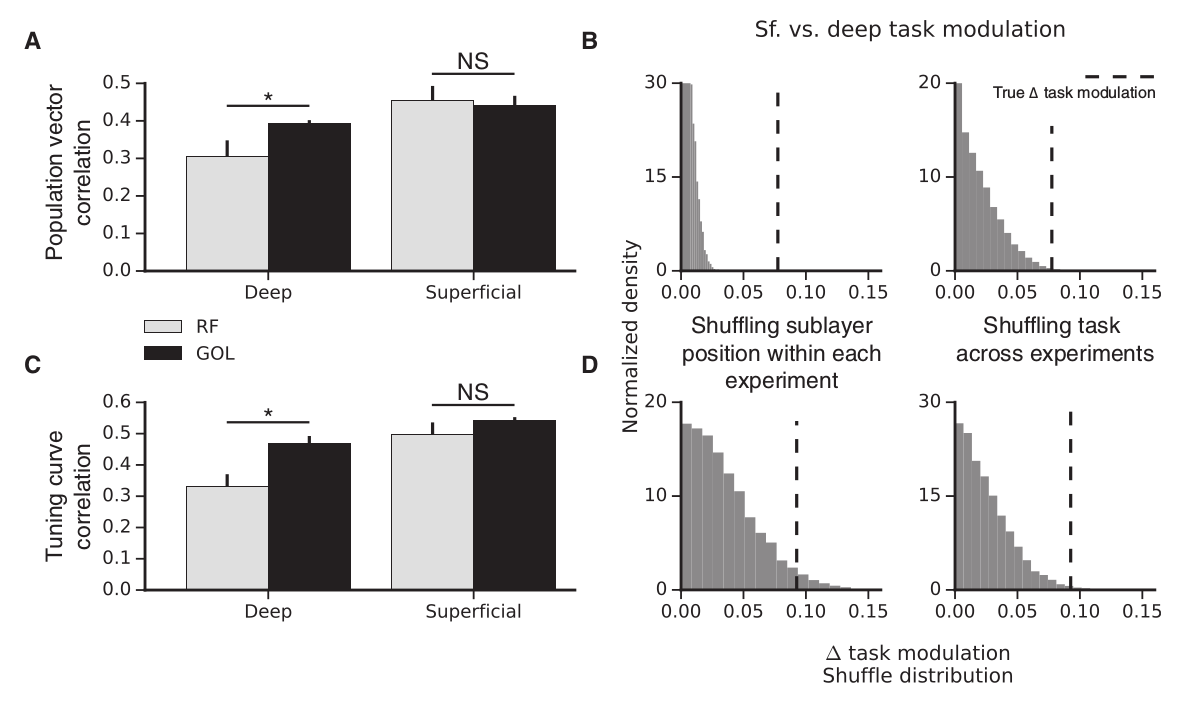
\includegraphics[width=0.8\textwidth]{applications/sf_deep_Fig4}
	\caption[Sublayer-Specific Modulation of Activity by the GOL Task]{Sublayer-Specific Modulation of Activity by the GOL Task.
	(A) Stability in the B-B condition of RF compared to session-to-session stability in GOL (similar elapsed time of $~$90~min.). Deep, but not superficial, CA1 PCs showed a significant increase in PV correlation in the GOL task as compared to RF (n~=~7 RF mice, 6 GOL mice; deep, p~$<$~0.05; superficial, p~=~0.36; Mann-Whitney U test). Error bars indicate mean $\pm$ SEM across animals.
	(B) The magnitude of the task modulation was compared across sublayers by performing two shuffling procedures: randomizing cell identity and randomizing task identity. Both comparisons suggested the magnitude of task modulation was greater for deep than for superficial cells (p~$<$~0.001, p~$<$~0.01).
	(C) The same analysis was performed with tuning curve correlation. Deep, but not superficial, CA1 PCs showed a significant increase in tuning curve correlation in the GOL task as compared to RF (n~=~7 RF mice, 6 GOL mice; deep, p~$<$~0.05; superficial, p~=~0.11; Mann-Whitney U test). Error bars indicate mean $\pm$ SEM across animals.
	(D) Both shuffles showed the magnitude of the task modulation was greater for deep than superficial (p~$<$~0.01, p~$<$~0.01).
	}
	\label{fig:other:sf-deep:stability}
\end{figure}

\begin{figure}
	\centering
	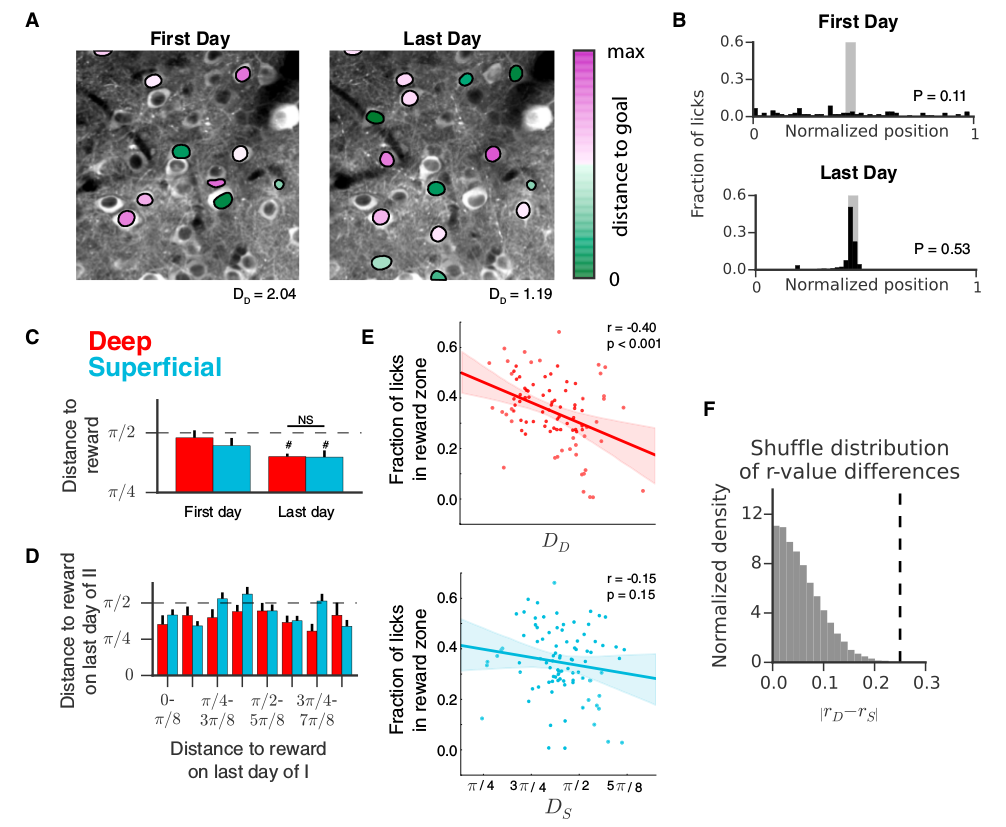
\includegraphics[width=0.8\textwidth]{applications/sf_deep_Fig6}
	\caption[Reward Zone Representation versus Performance on the GOL Task]{Reward Zone Representation versus Performance on the GOL Task.
	(A) Time-averaged images of the deep sublayer from two different recording sessions are shown in grayscale. Identified place cells from each session are overlaid and colored according to the distance of their centroid to the reward (green, near; purple, away). The mean distance to the reward zone is indicated (radians).
	(B) As in \autoref{fig:other:sf-deep:GOL}B, licking distributions from the two experiments corresponding to (A).
	(C) Mean distance of each place cell centroid to the reward on first and last days of the experiment. On the last day, the mean distance to reward was significantly different from the chance level of $\pi$/2 for both sublayers (dashed line; n~=~6 mice; one sample t-test; deep, p~$<$~0.001; superficial, p~$<$~0.05), but was not significantly different between sublayers (n~=~6 mice, p~=~0.95, paired t-test). Error bars indicate mean $\pm$ SEM across animals.
	(D) We did not detect a relationship between distance to reward at the end of condition II with distance at the end of I, sublayer, or with the interaction (type II ANOVA, n~=~172 deep, 336 superficial place cells, F(distance end of I)~=~0.10, p(distance end of I)~=~0.76; F(layer)~=~0.54, p(layer)~=~0.46; F(interaction)~=~0.11, p~=~0.74). The dashed line represents the mean distance expected in the case of a uniform place field distribution, and error bars indicate mean $\pm$ SEM across cells.
	(E) Fraction of licks in reward zone (P) plotted against D\sub{D} (top) and D\sub{S} (bottom). Individual points represent single recording sessions. The dashed line indicates the linear fit with the 95\% confidence interval shaded. We observed a significant relationship between D\sub{D} and P (n~=~91 sessions, r~=~0.40, p~$<$~0.001, Pearson's R), but not between D\sub{S} and P (n~=~91 sessions, r~=~0.15, p~=~0.15, Pearson's R).
	(F) In order to directly compare the sublayers' relationships to performance on the GOL task, we compared the magnitude of the difference in correlation coefficients (0.25, dashed line) relative to a null distribution. The true difference (dashed line) fell outside the shuffle distribution (p~$<$~0.001).
	}
	\label{fig:other:sf-deep:enrichment}
\end{figure}
\todo[inline]{Expand on sf-deep results}


% \part{The hippocampal output node}
% \input{chapter-pv}
% \input{chapter-sf_deep}

\part{Conclusions}
\chapter{Conclusions}
% \label{sec:conclusions}
\acresetall
\chapter{Conclusions}
\label{ch:conclusions}

\section{Summary}
In the preceding chapters I have laid out an understanding of memory in general, but also more specifically spatial-episodic memory, the structure in the brain that supports it (the hippocampus) and place cells as the functional units of these memories (\autoref{ch:intro:memory}).
I have explained the symptoms that define \scz/, particularly the cognitive deficits which are most relevant for functional recovery, yet least treatable, and identified some of the underlying genetic risk factors and proximate causes (\autoref{ch:intro:scz}).
I described the techniques that I employed inf my experiments as well and the tools I developed to run the experiments and analyze the data (\autoref{ch:intro:techniques}).
I next presented my primary thesis work; the characterization of hippocampal area CA1 pyramidal cell functional alterations during spatial learning in the \df/ mouse model of \scz/ (\autoref{ch:df}).
In addition, in collaboration I developed a Python package for the initial processing of Ca\super{2+} imaging data that we have released to the broader neuroscience community (\autoref{ch:sima}).
Supplementing my primary project, I also help characterize the \emph{in vivo} functional properties of long-range inhibitory projections from lateral entorhinal cortex to CA1, adult-born granule cells among the dentate gyrus granule cell population, and developmentally separable sub-populations of pyramidal cells within CA1 (\autoref{ch:other}).

It's worth noting that that while my main paper primarily looked to understand aberrant hippocampal activity in the \df/ mouse during spatial-reward learning task, my data also is interesting from the reverse perspective of understanding normal hippocampal function during a spatial-reward learning task.
We have shown that the \df/ mouse is a model of impaired global remapping (context stability) and goal-related remapping (enrichment), two fairly complicated properties of neuronal circuits that would otherwise be very difficult, if not impossible, to manipulate.
From this perspective, my data provides evidence that inducing global remapping or preventing reward-zone place cell enrichment impairs spatial-reward memory.

% \subsection{What we learned about memory}

% It's impossible to talk about declarative memory without quickly getting to discussions of the \ac{HPC}.
% By performing some of the first functional \emph{in vivo} imaging experiments in the \ac{HPC} I characterized the \emph{in vivo} activity of novel circuit elements and showed how this activity mapped on to behavior.



% \subsection{What we learned about \scz/}

% Minor changes to context resulted in global remapping in \df/ mice, lending support to the idea of \scz/ as a disorder of aberrant salience.

\section{Future directions}

% There remains several open questions directly related to my work as well as new related areas of research.

% follow-up experiments 
% new experiments
% new compartments
% new mice

\subsection{Context generalization}
My \ac{GOL} task tested two fundamentally different aspects of spatial memory: How do spatial maps change in response to small changes to the environment (Condition~I \& II)? and How do spatial maps support the encoding of salient reward locations (Condition~II \& III)?
I found an interesting differential effect between WT and \df/ mice in both of these tasks, so it would be interesting to explore each of these in more detail.
In particular, my context remapping results suggests that the \df/ mis-attend to stimuli that the wildtype mice ignore, which manifests as an over-separation of similar contexts as seen by impaired task performance and also the global remapping of spatial maps between the two similar contexts.
This could be looked at in more detail by systematically modifying the two contexts to have varying degrees of symmetry and look at similarity of spatial maps between the two contexts while performing a context discrimination task.

\subsection{Interneurons}
Hippocampal area CA1 consists not only of a dense pyramidal cell layer, but also diverse populations of local GABAergic interneurons which control pyramidal cell spiking \citep{Freund1996}.
Two main classes of pyramidal cell-targeting GABAergic neurons -- dendrite-targeting (e.g. somatostatin-positive; SST+) and soma-targeting (e.g. parvalbumin-positive: PV+) interneurons -- have been shown to directly modulate pyramidal cell burst spiking and theta phase repsectively \citep{Royer2012, Lovett-Barron2012}.
A third potentially interesting classification of interneurons in the \ac{HPC} are the interneuron-targeting vasointestinal peptide expressing (VIP+) interneurons, which are less well understood, but can drive \ac{HPC} pyramidal cell activity though disynaptic disinhibition \citep{Chamberland2012}.
\todo[color=yellow]{Expand on VIP cells}
Importantly, an excitatory-inhibitory imbalance has also been implicated as a possible root cause of \scz/ progression (see \autoref{sec:intro:scz:glutamate}).
Goal oriented learning-related reorganization of hippocampal CA1 interneuron activity has been recently demonstrated \citep{Dupret2013}, suggesting that CA1 GABAergic interneuron activity is closely tied to learning-related remapping of place cell ensembles, but the role of genetically-identified \ac{HPC} GABAergic inhibitory circuits during normal and diseased learning and memory has not been characterized.
In particular, the paper by \citeauthor{Dupret2013} shows that interneuron activity evolves with pyramidal cell activity as learning progresses and place cells enrich the reward location.
It is tempting to infer that interneuron activity is shaping pyramidal cell activity profiles, as it is possible that local interneurons could provide the needed signal to shift place cell firing towards the reward location.
By recording the activity of dendrite-targeting and soma-targeting interneurons during the \ac{GOL} task I can look for altered activity during Condition~III, when the \df/ mice failed to show any reward enrichment, and also performed poorly on the task.
\todo[color=yellow, inline]{Include mention of prelim VIP data?}

\subsection{Imaging during alternate hippocampus-dependent behaviors in \df/ mouse}
Goal-oriented learning, as a test of spatial-episodic memory, was the first behavior -- beyond simple random-foraging tasks -- that we attempted to train the head-fixed \df/ mice to perform.
It would also be very interesting to analyze behaviors related to other cognitive domains with well-known deficits in the \df/ mice.
The \df/ mice have a well-established deficit in contextual fear conditioning \citep[CFC,][]{Stark2008} -- they freeze less than wildtype mice -- and we have already adapted CFC for head-fixed imaging \citep[hfCFC,][]{Lovett-Barron2014}.
Our hfCFC uses an airpuff to the snout, instead of a foot shock, as the unconditioned stimulus (US) and lick suppression, instead of freezing, as the conditioned response (CR), so we would need to confirm that the \df/ still showed a behavioral deficit with this potentially milder US.
Based on the work by \citeauthor{Moita2004}, I would expect to see place cell remapping selectively induced in the wildtype mice in the conditioned context, but not in the \df/ mice.
In addition, we have shown that SST+ interneurons in CA1 effectively filter out the CS from the representation of the conditioned context \citep{Lovett-Barron2014}, so disrupted interneuron activity in the \df/ mice could lead to contamination of the conditioned context representation in the \ac{HPC} by the US, leading to the observed deficit in freezing.
This would also be generally consistent with my finding that the \df/ mice are differentially affected by small changes to the contextual environment (\autoref{sec:df:results:context}) and the \scz/ conceptual framework that suggests that mis-attribution of salience may be the the fundamental underlying dysfunction \citep{Kapur2003a, VanOs2009}.

Another interesting behavior for future study is prepulse inhibition (PPI), where the magnitude of the acoustic startle response to a loud noise is markedly reduced by preceding the tone with a milder stimulus.
The \df/ mouse shows decreased PPI, and this behavior involves the septo-hippocampal cholinergic projection in particular \citep{Koch1996, Swerdlow2001}.
This task should be fairly straightforward to establish as a head-fixed paradigm.
As place cells and running activity would not necessarily be relevant for this task, I could instead use an immobilization chamber in place of the treadmill that I used throughout my previous experiment.
Mice quickly adapt to this form of restraint and other members of our lab regular make use of this technique.
The aversive stimulus could be either an airpuff as we've used in the past, or a mild shock delivered through the immobilization chamber.
By imaging the cholinergic septo-hippocmapal projections in HPC area CA1 we could determine if they are altered in the \df/ mouse model, and if so, we could potentially attempt to correct the aberrant activity using optogenetics or pharmacogenetics approaches.

\subsection{Sharp wave-ripples in \df/ during goal-oriented learning}
We looked at baseline \ac{SWR} in WT and \df/ mice and found aberrant activity characterized by increased high-frequency power and an increased number of \ac{SWR} events (\autoref{sec:df:results:SWR}).
This is a very interesting initial finding that could be a fundamental aspect of memory deficits in this mouse.
SWRs are fundamental to the consolidation and recall of episodic memories \citep[reviewd in,][]{Buzsaki2015}.
They have specifically been shown to increase in frequency following rewarded trials in a spatial memory task \citep{Singer2009}.
In the work by \citeauthor{Dupret2010a} which is conceptually similar to my \ac{GOL} task, the authors found that the the fraction of cells that participated in SWRs during the task (the more cells `remembering') and the similarity of place maps reactivated after the task during SWRs with the place maps near the reward locations during the task (the better they `remembered' the reward) correlated with task performance.
By recording \ac{SWR} activity during and immediately after our \ac{GOL} task we could  look for disruptions in SWRs directly related to task performance.
Based on our initial findings and the above mentioned work, I would hypothesize to see aberrant \ac{SWR} activity specifically after the task, during the time most critical for consolidation to long-term memory.
This could explain why we see learning similar to WT mice in the \df/ mice during the day, but a large deficit following the overnight period (\autoref{fig:df:performance_by_session_in_day}).

\subsection{Reward cells}
Recent work by several labs has identified a small population of \textsc{reward cells} among the place cell population in CA1 \citep{XXXX}.
In spatial reward learning tasks, these cells follow the reward location as it moves and their firing has been shown to predict reward memory -- their activity directly precedes the onset of reward licking \citep{XXXX}.
I actively searched through my data for evidence of reward cells and was not able to find any.
This cell population would be interesting to study in general, as the formation and stability of this cell population over time has not been throughly investigated and they could have large implications for spatial reward learning.
Also, in the \df/ mice, their absence might also be reflective of their impaired task performance.
To facilitate finding these cells, it would be helpful to modify the \ac{GOL} task to include more than 2 reward locations.
Instead of changing the context and then the reward, I could instead change the reward twice.
This would help to identify cells that actually represented all three reward locations at the end of each Condition.

\subsection{Explore place field shift result}
How do place cells throughout the environment coherently shift their firing fields towards the reward location (Figures \ref{fig:df:shift_fit} \& \ref{fig:df:param_swap})?
The underlying mechanism driving this coherent shift remains unknown.
Our result shows a symmetric shift towards the reward location, so some signal -- which could be local to CA1 or from another brain region -- needs to anticipate the reward position in order to shape the firing of place fields that precede the reward.
We do see anticipatory licking leading up to the reward location that predicts tasks performance (\autoref{fig:conclusions:anticipatory_licking}), so this information is clearly represented somewhere.
Three possibilities that I would like to further investigate are that enrichment originates in the entorhinal cortex is inherited by CA1, that neuromodulatory signals shape the tuning curves, or the local inhibitory circuit shifts firing fields towards the reward.
\begin{figure}
	\centering
	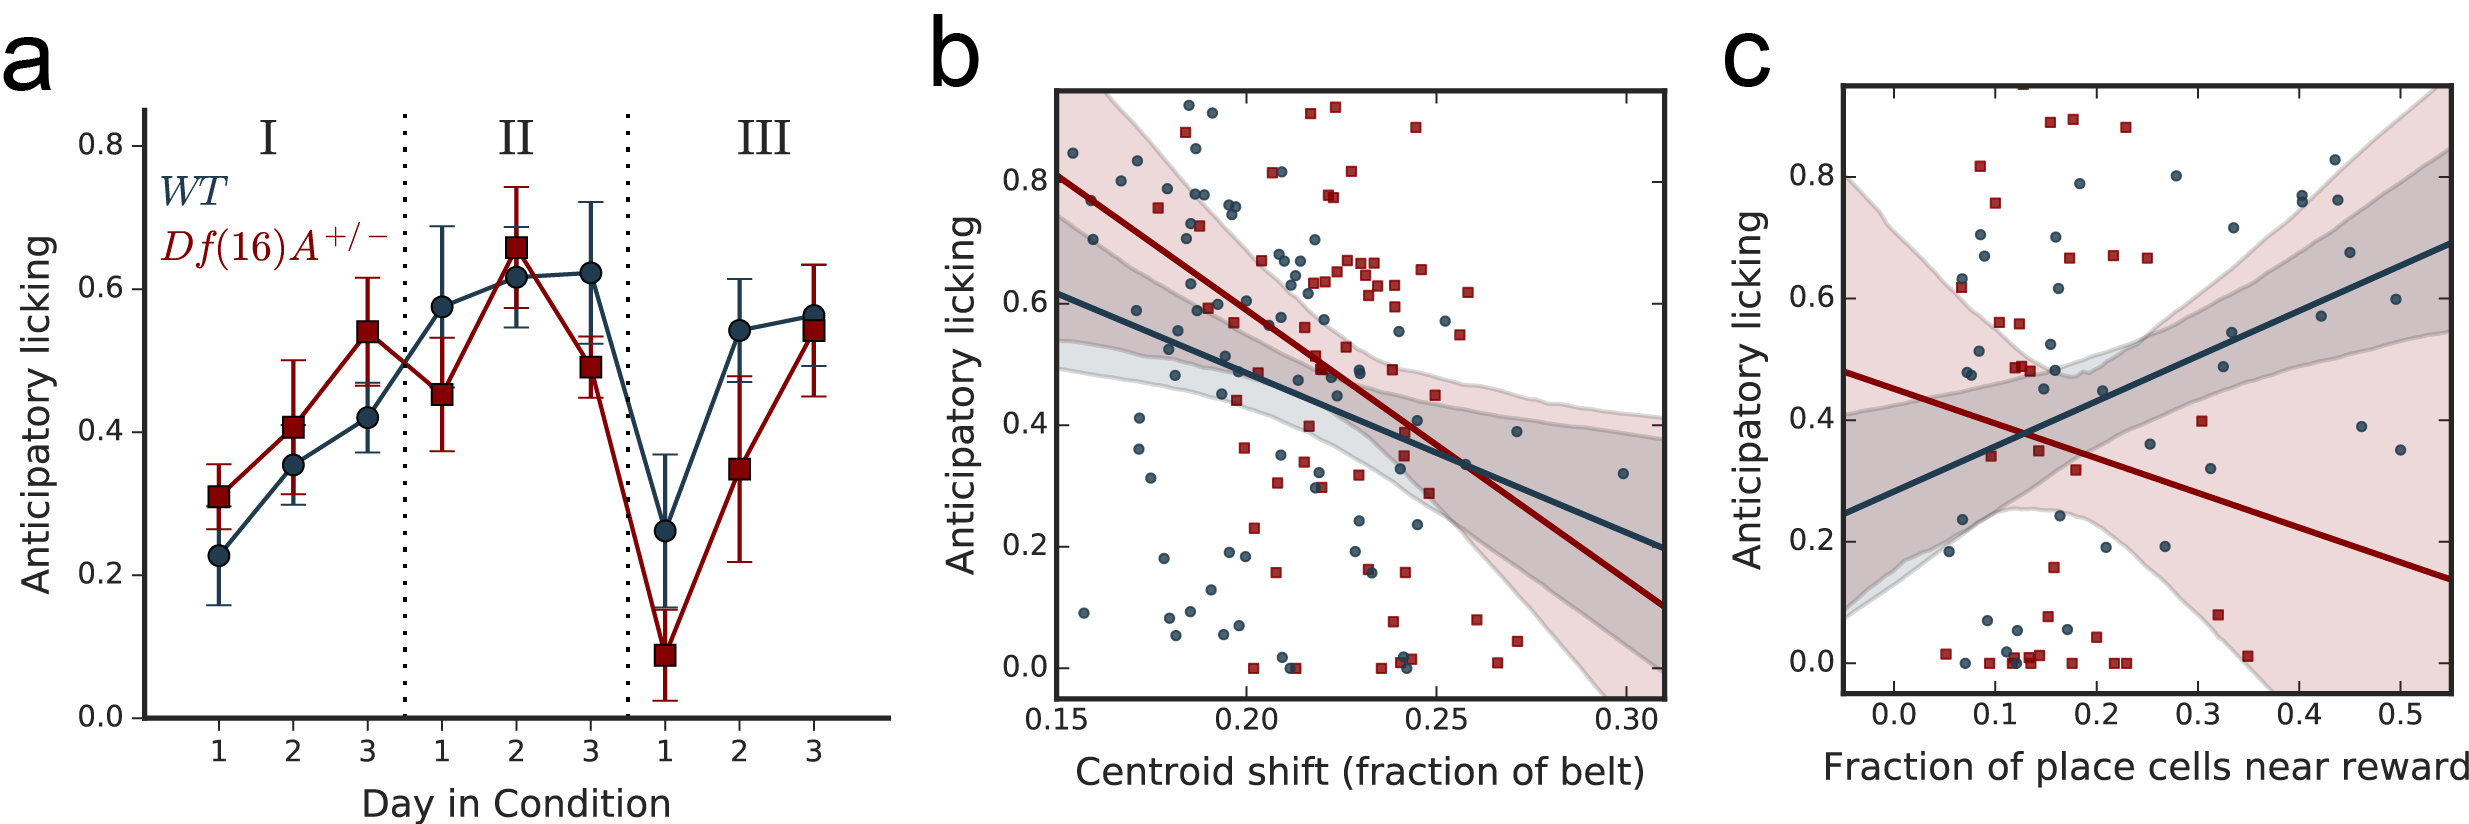
\includegraphics[width=0.9\textwidth]{df/FigSX_anticipatory_licking}
	\caption{}
	\label{fig:conclusions:anticipatory_licking}
\end{figure}
% \todo{include nucleus acumbens/VTA}

Hippocampal area CA1 receives a direct project from the entorhinal cortex via the temporoammonic pathway, which could shape their activity in a task- and learning-dependent manner. Grid cells in the medial entorhinal cortex are thought to contribute to a cognitive map of space by providing a metric framework for direction and distance \citep{Hafting2005, Jeffery2015a} and these cells directly project to hippocampal area CA1 \citep{Zhang2013}, though the nature of their influence on CA1 place cell activity is currently debated \citep{Wills2010, Langston2010, Koenig2011, Brandon2011a}. Recent studies \citep{Krupic2015a, Stensola2015a} have found evidence for warping of grid spacing to salient anchors points (walls), so it is tempting to speculate about a similar warp of grid cell spacing by the learned reward position.
While we did not record from area CA3 cells in the current study, previous studies \citep{Dupret2010a} have shown similar goal-directed remapping in CA1, but no remapping in CA3, leading to the possibility that area CA1 place cell activity is driven by stable CA3 representations and updated with environmental sensory input (border cells) and self-motion cues (grid cells) from the entorhinal cortex \citep{Bush2014a}.
Particularly, an increasing gradient of grid spacing centered about the reward would provide the perception of slower movement, thus delaying the firing of cells tuned to distance from boundaries and shifting all place cells towards the reward. The nature of border cells in a one-dimensional head-fixed environment is not entirely obvious, though there are salient belt fabric transitions that could similarly anchor a cognitive reference frame.
This interpretation predicts that after reward learning, a given grid module will have an increased scale, with spacing maximal farthest away from the reward (largest shift) and smallest near the reward (smallest shift).
Also, under conditions of grid cell map warping, we would expect a correlation between the local density of grid fields and the density of place cells.
By recording either grid cells directly from the medial entorhinal cortex or grid cell axons that project to CA1, we could directly test these predictions.

\todo[inline, color=yellow]{CA1 as source of enrichment, INs/neuromodulatory}
% Alternatively, CA1 could itself be the source of enrichment if 

\subsection{Long term stability in place cell population}
One of my first experiments with the \df/ mouse was to look at the long-term stability of CA1 spatial maps in a similar manner as \citeauthor{Ziv2013}.
Mice were trained to run head-fixed on our same cue-rich multi-fabric belts as I used in the \ac{GOL} task, but only for 1 session each day and the water reward was presented non-operantly once per lap at the same location every day.
I recorded CA1 pyramidal cell activity for at least 6 days without changing any aspects of the task.
By looking at the stability between spatial maps at progressively longer elapsed intervals I found that while the wildtype stability decreased from 1 day elapsed to 5 days elapsed, the \df/ spatial maps were surprisingly rigid for the entire 6 days (\autoref{fig:conclusions:chronic_stability}).

\begin{figure}
	\centering
	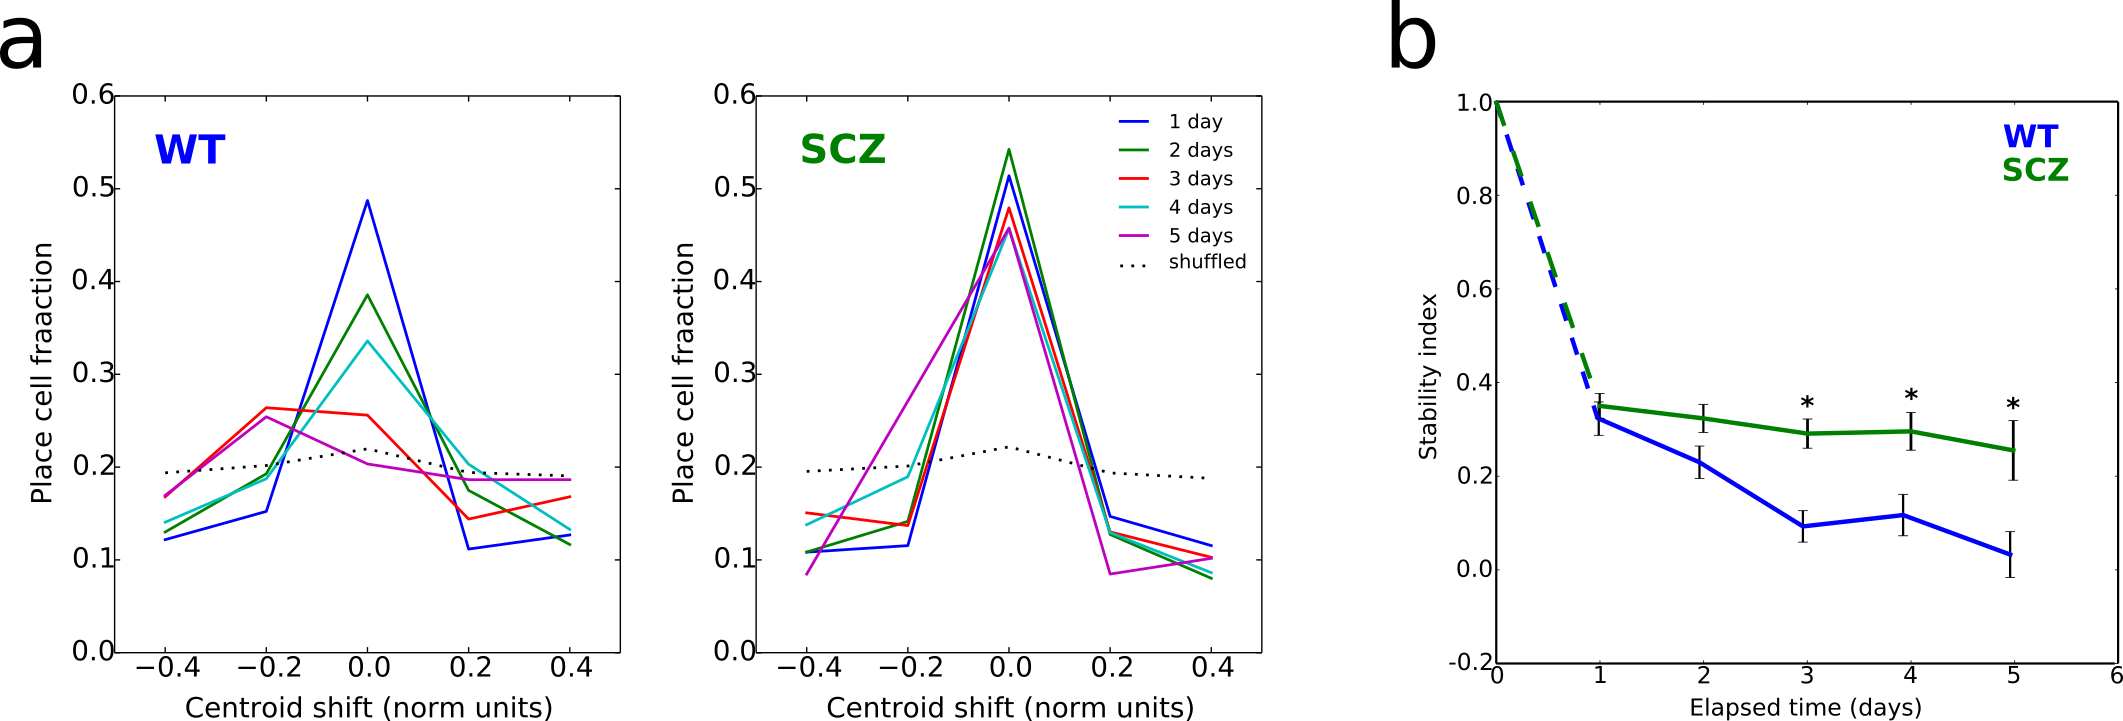
\includegraphics[width=0.9\textwidth]{df/chronic_stability}
	\caption{}
	\label{fig:conclusions:chronic_stability}
\end{figure}

\citeauthor{Ziv2013} actually found the wildtype mice to be more stable than what I observed, but I think this can be contributed to differences in task protocol.
In their task, mice were running in an already familiar environment, so the stability observed was reflective of an already stabilized spatial map.
In contrast, in our task the belt that conveys all of the spatial information was novel on day~1, therefore we observed the normal stabilization that occurs over the first few days of exposure to a novel environment.
This interpretation suggests that the \df/ mice immediately stabilize their spatial maps so that they don't allow for the normal stabilization process to occur.

This data needs further follow-up to completely interpret the results.
There was really no spatial learning in this version of the task.
Mice received water as long as they continued to run, it was delivered automatically every lap, and they didn't need to remember where that location was.
The first experiment I would run would be to change the reward schedule to require learning and memory.
Instead of a non-operant reward every lap, I would make it similar to the \ac{GOL} task; one rewarded zone where the water is only delivered if the mice actually lick there.
In this case I would expect to see several factors alternatively driving stability or rigidity.
First, wildtype mice showed a task-dependent stabilization from day-to-day, so we might see this effect over longer timescales as well.
Second, in Condition~III of my \ac{GOL} task I observed place cell enrichment of the reward location in the wildtpye mice, which could manifest as transient instability as cells remap to the reward, but then increased stability as they stabilize.
Finally, I observed neither of those effects in \df/ mice, so I don't necessarily expect this change to affect the stability of the \df/ place fields.

In addition, to see if the decreased stability in the wildtype mice relative to \citeauthor{Ziv2013} is truly due to environment novelty, we could either over-train the mice on the same belt on which we will eventually record place cell activity, or extend the protocol to 10 or more days so that we can alternatively discard the first few days and look at long-term stability relative to day 3 or 4.
I would expect to see increased stability in the wildtype mice, back to the level observed initially in the \df/ mice.
Assuming that both of these proposed manipulations increase stability in the wildtype mice, but don't affect the already increased \df/ stability, this would confirm an aberrantly fast place map rigidity in novel environments, and would suggest deficient novelty signaling in the \df/ mice, which may be linked to aberrant neuromodulatory signaling of novelty or generally with the proposed role of CA1 in novelty detection \citep{Li2003d, Barry2012c, Larkin2014, Nitz2004}.

\begin{figure}
	\centering
	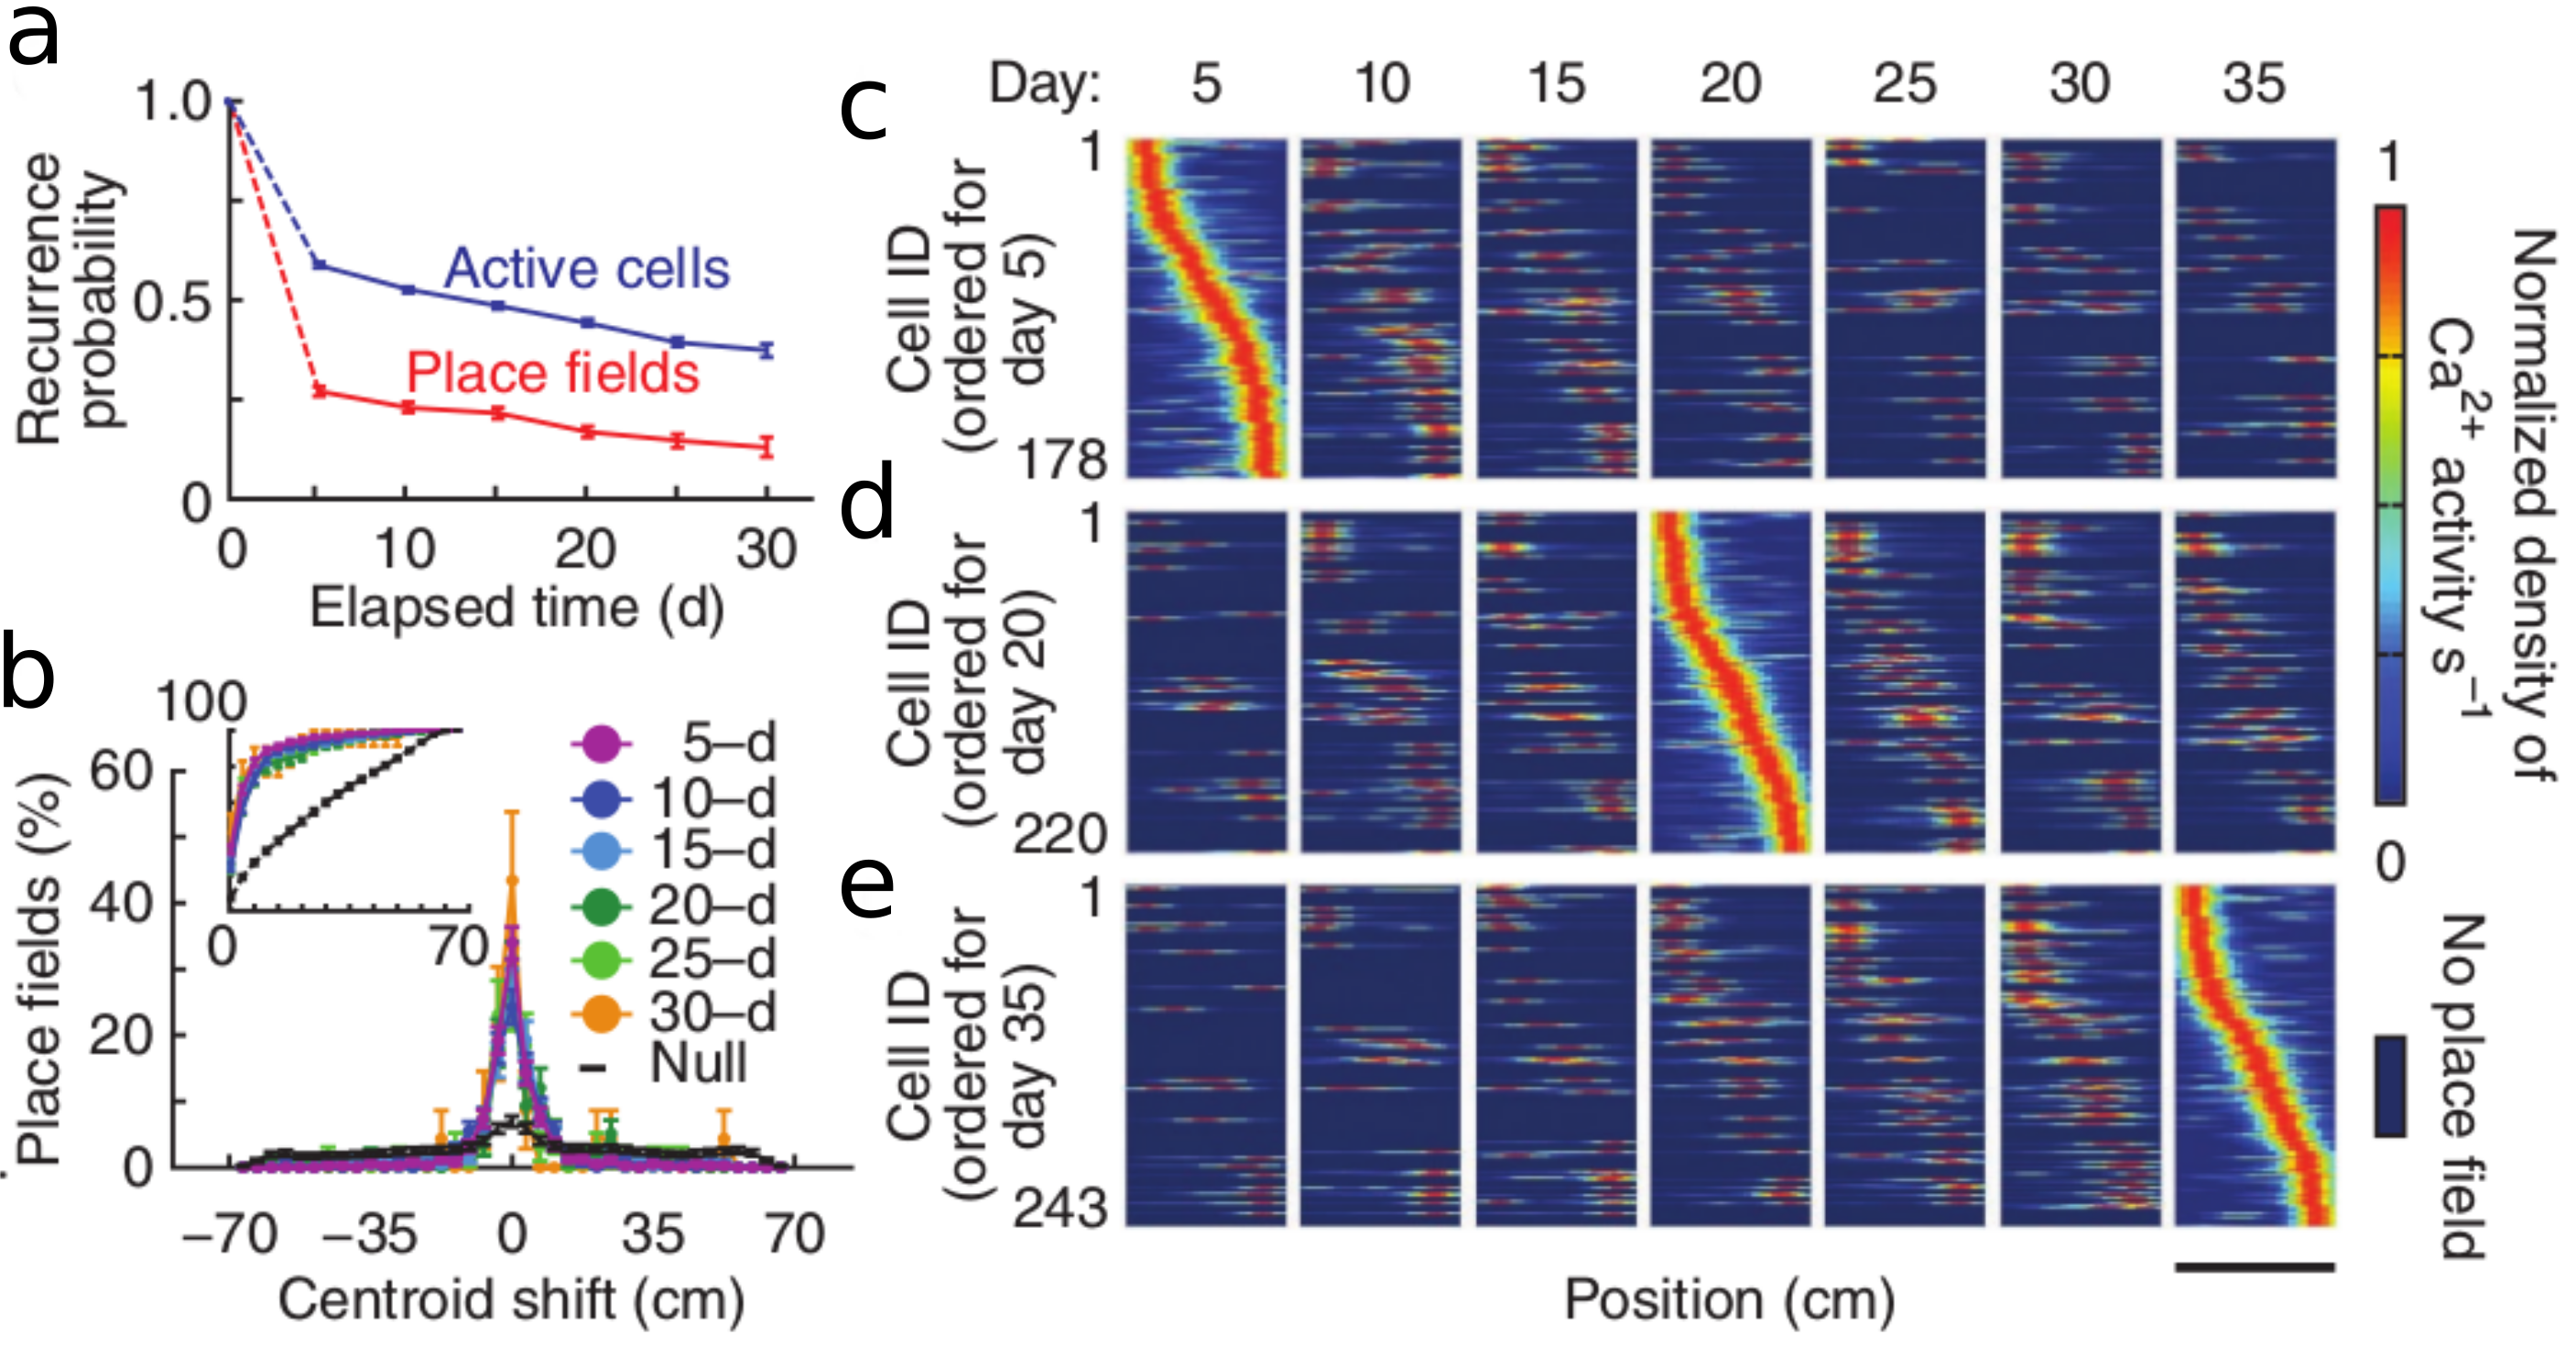
\includegraphics[width=0.75\textwidth]{intro/Ziv2013_stability_edit}
	\caption[Place field stability in Ziv et al.]{Place fields are spatially invariant and temporally stochastic while preserving a stable representation at the ensemble level.
	(a) If a cell had Ca\super{2+} activity in one session, the odds (blue data) that it also did in a subsequent session declined with time. If a cell had a statistically significant place field in one session, the odds (red data) that it had a place field in a subsequent session also declined with time. Mean~$\pm$~s.e.m.
	(b) Distributions of centroid shifts (colored by days between sessions, mean~$\pm$~s.e.m.) were indistinguishable (Kolmogorov-Smirnov test, P~$\geq$~0.17), sharply peaked at zero and highly distinct from the null hypothesis that place fields would randomly relocate (P~=~$4\times10^{-67}$, Kolmogorov-Smirnov test). Inset, cumulative histograms of shift magnitudes; 74-83\% were $\leq$7~cm. Median shift (3.5~cm) was much less than the median place field width (24~cm).
	(c-e) Place-field maps for cells found on multiple days, ordered by place fields' centroid positions on day~5 (c), day~20 (d) or day~35 (e). Data pooled across four mice.
	Reproduced from \citet{Ziv2013}.}
	\label{fig:conclusions:ziv_stability}
\end{figure}

\subsection{Neuromodulators in the \acl{HPC} of \df/ mice}
Place cell stability can be affected by salience, novelty, and attention, which has been shown to act through neuromodulatory inputs, including dopamine and acetylcholine.
In addition both dopamine and acetylchline have been implicated in \scz/ disease progression.
To search for aberrant salience/novelty/atention signaling in the \df/ mice I could directly image the activity of the dopaminergic and cholinergic axons projecting from the ventral tegmental area and medial septum, respectively, to area CA1 of the \ac{HPC}.
% and then use a combination of pharmacological, optogenetic and pharmacogenetic manipulations of each network component in order to dissect out the underlying circuit mechanisms of spatial memory deficits in the SCZ mutant mice.

Both principal neurons and local GABAergic interneurons are targeted by afferents from neuromodulatory nuclei, including cholinergic and GABAergic projections from the medial septum (MS) \citep{Klausberger2008}, serotonergic and glutamatergic projections from the raphe nuclei \citep{Varga2009}, dopaminergic projections from the ventral tegmental area (VTA) \citep{Gasbarri1997} and noradrenergic projections from the locus coeruleus \citep{Foote1983}.
Of these neuromodulatory projections, the dopaminergic-VTA and cholinergic-MS projections are of particular interest, since there is already extensive literature relating dopamine to \scz/ \citep{Davis1991} and the cholinergic projection is involved in normal hippocampal learning and memory \citep{Parent2004}.
Despite these well-characterized features of hippocampal neuromodulation, it remains unknown how the function of these circuits are altered in \scz/ during hippocampal-dependent behaviors.


%%%
%%% Appendices
%%%
% \part{Appendices}
% \appendix
% \input{sample-appendix}
% \input{sample-appendix}

%%%
%%% Bibliography
%%%
% \part{Bibliography}
\addcontentsline{toc}{chapter}{Bibliography}
\singlespacing
\bibliographystyle{neuron} 
\bibliography{library}

\end{document}
